\documentclass[11pt]{article}
\usepackage[T1]{fontenc}
\usepackage[utf8]{inputenc}
\usepackage{lmodern}
\usepackage{amsmath,amssymb,amsthm,mathtools,mathrsfs}
\usepackage[margin=1in]{geometry}
\usepackage{booktabs,longtable,array}
\usepackage{graphicx,tikz}
\usepackage{microtype}
\usepackage[hyphens]{url}
\usepackage[colorlinks=true,linkcolor=blue!50!black,citecolor=blue!50!black,urlcolor=blue!50!black]{hyperref}
\usepackage{bookmark}
\makeatletter
\renewcommand*\l@subsection{\@dottedtocline{2}{1.5em}{3.6em}}
\renewcommand*\l@subsubsection{\@dottedtocline{3}{3.8em}{4.6em}}
\makeatother
\hypersetup{pdfauthor={OpenAI},pdftitle={Polynomial vacuum representations and bridge mass for honeycomb walks}}
\allowdisplaybreaks[2]
\numberwithin{equation}{section}
\newtheorem{theorem}{Theorem}[section]
\newtheorem{lemma}[theorem]{Lemma}
\newtheorem{proposition}[theorem]{Proposition}
\newtheorem{corollary}[theorem]{Corollary}
\newtheorem{claim}[theorem]{Claim}
\theoremstyle{definition}
\newtheorem{definition}[theorem]{Definition}
\theoremstyle{remark}
\newtheorem{remark}[theorem]{Remark}
\DeclareMathOperator{\Pf}{Pf}
\DeclareMathOperator{\Tr}{Tr}
\DeclareMathOperator{\Res}{Res}
\DeclareMathOperator{\diam}{diam}
\DeclareMathOperator{\dist}{dist}
\DeclareMathOperator{\supp}{supp}
\DeclareMathOperator{\rank}{rank}
\DeclareMathOperator{\Span}{span}
\title{Polynomial vacuum representations\\and bridge mass for honeycomb walks}
\author{OpenAI}
\date{September 26, 2026}
\pdfinfoomitdate=1
\pdftrailerid{}
\pdfsuppressptexinfo=15
\begin{document}
\maketitle
\begin{abstract}
We prove that, under the all-length critical measure, a honeycomb bridge crossing a strip of $h$ layers, with its initial port fixed and its terminal port free, has mean length $h^{4/3+o(1)}$. We also obtain central visit probability $R^{-2/3+o(1)}$ and mean length $R^{4/3+o(1)}$ for macroscopic free-boundary chords in a regular hexagon.
\end{abstract}
\tableofcontents
\section{Critical bridge length and a polynomial polygon observable}
\label{sec:pv:introduction}

A walk can cross a wide strip while making many returns to a much smaller
region. Its total crossing weight therefore does not determine its mean
length. We study this distinction for critical self-avoiding walks on the
honeycomb lattice. Our initial boundary point is fixed and the terminal
point is summed over the opposite wall. The main result is a mean-length
exponent of $4/3$ under this all-length measure.

We use the honeycomb lattice dual to the equilateral triangular tiling of
side one. Its edges have length $1/\sqrt3$. A \emph{port} is the midpoint
of an edge cut by a tiling line. A path between ports visits distinct
honeycomb vertices, and its length $|\gamma|$ is their number. Its critical
weight is $x_*^{|\gamma|}$, where
\[
 x_*=(2\cos(\pi/8))^{-1}=(2+\sqrt2)^{-1/2}.
\]
The terminal half-edges have no additional weight. A strip of $h$ layers
has physical height $h\sqrt3/2$. With a bottom source at horizontal
coordinate zero, its attainable top ports lie in $\mathbb Z+h/2$.
Write $\mathcal B_h(e)$ for the paths confined to that strip from the
source to top port $e$, and put
\[
 b_h(e)=\sum_{\gamma\in\mathcal B_h(e)}x_*^{|\gamma|},\qquad
 b_h=\sum_e b_h(e),\qquad
 \ell_h=\sum_e\sum_{\gamma\in\mathcal B_h(e)}
 |\gamma|x_*^{|\gamma|}.
\]
Thus $\ell_h$ is a first-length insertion, rather than a partition
function conditioned on one length. The bridge law assigns each such
path probability $x_*^{|\gamma|}/b_h$.

\begin{theorem}[Strip mass and bridge length]\label{thm:pv:bridge}
As the integer layer height $h$ tends to infinity,
\[
 b_h=h^{-1/4+o(1)},\qquad
 \ell_h=h^{13/12+o(1)},\qquad
 \mathbb E_h|\gamma|=h^{4/3+o(1)}.
\]
All three sums are finite. These exponents are unchanged if the paths
are also confined to horizontal distance $h\log^2h$ from their initial
port.
\end{theorem}

Throughout, $f(h)=h^{a+o(1)}$ means that $f(h)>0$ for all sufficiently
large $h$ and $\log f(h)/\log h\to a$. In particular, the theorem gives
subpower precision; it does not assert bounds by fixed multiples of the
displayed powers. Its last conclusion uses a logarithmically widening
strip, and is distinct from confinement to a fixed multiple of $h$.

The same proof determines a finite free-boundary chord law. In a regular
lattice hexagon of integer side $R$, sum critical weights over paths
joining ordered boundary ports, retaining only paths of diameter at
least $R/10$. Reversal gives a second ordered path and leaves the
normalized law unchanged. Denote the resulting probability by
$\mathbb P_R$.

\begin{theorem}[Hexagon visits]\label{thm:pv:hexagon}
The mass normalizing $\mathbb P_R$ is $R^{3/4+o(1)}$. Uniformly at
vertices in the concentric hexagon of side $R/3$,
\[
 \mathbb P_R(v\in\gamma)=R^{-2/3+o(1)}.
\]
The corresponding upper bound holds at every vertex, and
$\mathbb E_R|\gamma|=R^{4/3+o(1)}$.
\end{theorem}

There is an intermediate strip law in which the distinction between
arches and bridges matters. An \emph{arch} returns to the wall where it
started. From one fixed bottom port, allow both arches and bridges and
condition the path to reach at least $\vartheta h$ layers above the
bottom, where $0<\vartheta<1/2$ is fixed.

\begin{proposition}[Mixed exits]\label{prop:pv:mixed}
The conditioned event has unnormalized mass $h^{-1/4+o(1)}$ and
first-length mass $h^{13/12+o(1)}$. Hence its normalized mean length is
$h^{4/3+o(1)}$. Restricting horizontal distance to $h\log^2h$ preserves
these exponents. The total first-length mass of all exits, without the
height condition, is at most $h^{13/12+o(1)}$.
\end{proposition}

The mixed mean follows directly from a finite vertex-visit identity.
The bridge mean requires an additional argument that transfers mass
from returning arches to crossing paths. It is this argument, rather
than normalization alone, that completes Theorem~\ref{thm:pv:bridge}.
Both theorems concern means in positive critical measures; fixing a
length or prescribing both ports asks a different question.

\subsection{Critical crossing mass and related laws}

Nienhuis's analysis of the dilute $O(n)$ model led to the honeycomb
critical point and the critical-exponent predictions associated with planar
self-avoiding walk~\cite{Nienhuis1982}. Duminil-Copin and Smirnov proved
the connective constant $\sqrt{2+\sqrt2}$ by a parafermionic observable
and its boundary cancellation~\cite{DuminilCopinSmirnov2012}. We use that
local cancellation, prove the particular finite flux identities needed
here, and keep the visited-vertex convention explicit.

The sharper crossing-mass power $h^{-1/4}$ is recorded as a prediction
in \cite[Section~4]{DuminilCopinSmirnov2012}. Beaton, Bousquet-M\'elou,
de Gier, Duminil-Copin and Guttmann proved that the critical bridge
mass tends to zero~\cite{BeatonEtAl2014}. Glazman and
Manolescu~\cite{GlazmanManolescu2017} obtained a quantitative subsequence
bound, as well as invariance of boundary two-point functions in
columnwise rhombic half-planes with Yang--Baxter weights. Krachun and
Panagiotis proved a polynomial upper bound on the critical bridge
mass~\cite{KrachunPanagiotis2026}. These crossing-mass estimates do not
by themselves control a first-length insertion. In particular, the
all-length means considered here are distinct from displacement laws
for uniform walks of a fixed length.

The companion paper \cite[Theorem~1.1]{DiskTransfer2026} proves the same
all-length bridge-mean exponent and retains it inside a fixed corridor
of sufficiently large width $Ch$. It also obtains bridge mass
comparable to $h^{-1/4}$. Our proof of the strip and hexagon results is
given independently below; we do not use the companion's mean theorem.

\subsection{A polygon observable and its construction}

The first-length insertion will be obtained by summing the mass of paths
through a marked vertex. The corresponding algebraic observable counts
surrounding polygons instead of paths. Identify horizontal translates by
$2n$, forming an infinite honeycomb cylinder, and mark two face centers
on one horizontal cut, separated by $n$ sites. Let $F_n(\eta)$ sum over
systems of pairwise vertex-disjoint unoriented simple polygons, each
separating the two marks. A polygon $P$ has weight $\eta x_*^{|P|}$, and
the empty system has weight one. Each polygon crosses the intervening
marked interval, so this is a polynomial in $\eta$; its coefficients are
convergent weighted sums over polygon shapes on the infinite cylinder.

\begin{theorem}[Normalized separator pairing]\label{thm:pv:puncture}
For every compact set $K\subset\{s\in\mathbb C:|\Im s|<\pi\}$ there
is $C_K<\infty$ such that, for all $n\ge1$ and $s\in K$,
\[
 |F_n(2\cosh s)|\le
 C_K n^{1/6+2\Re(s^2)/(3\pi^2)}.
\]
There is a disk about $\eta=0$, independent of $n$, in which $F_n$ has
no zeros. For each fixed $k$, the order-$k$ Taylor coefficient of
$\log F_n$ at zero is $O_k(1+\log n)$. At the positive fugacity two,
\[
 F_n(2)=n^{1/6+o(1)}.
\]
\end{theorem}

To construct $F_n$, record at each of $N=2n$ edges on a cylinder cut
whether the edge is empty or carries either orientation of a path.
The oriented pieces carry local turn phases, and adding a row acts
linearly on the resulting three-state tensors. We construct a common
eigenvector of eigenvalue one whose entries are polynomials in
parameters attached to those edges. Dividing by its empty component
gives the normalized \emph{vacuum}: at the physical honeycomb parameters
its entries are the amplitudes of the half-cylinder path systems.
Pairing two such states with a twist between the marked faces cancels
nonseparating loops and assigns each separating loop weight
$\eta=2\cosh s$.

The normalization $F_n(0)=1$ is essential. Both the finite color formula
for the numerator and the Pfaffian denominator have exponential growth
in $n^2$. The polynomial power survives only after those factors cancel
in the same normalization. Uniformity for complex $s$ also has a
positive-measure consequence: the zero-free disk controls polygon
incompatibilities when the cylinder is opened into the plane.

This construction uses polynomial exchange equations and reductions at
special values of neighboring parameters. Di Francesco and
Zinn-Justin~\cite{DiFrancescoZinnJustin2005} used these ideas for a
multiparameter sum rule in the dense $O(1)$ model. Garbali and
Nienhuis~\cite{GarbaliNienhuis2017Ground,GarbaliNienhuis2017Sum}
developed $q$KZ and fusion recurrences and determinant expressions for
the dilute $O(1)$ model with open boundaries; they also discussed the
polynomial construction at loop weight zero. Here the periodic
twist-$i$ state, its empty-component normalization and its physical
separator pairing are constructed explicitly. The companion's disk
states represent the same homogeneous separator sum;
Section~\ref{c01-c1-the-balanced-puncture-observable} compares the common
scalar polynomial and physical observable. The inhomogeneous vectors
and normalized complex estimates here are proved separately.

The local transfer weights belong to the dilute-loop and three-state
vertex-model setting of Zhou and Batchelor~\cite{ZhouBatchelor1997}.
Related finite recurrences and corner-transfer calculations for
restricted-height dilute models were developed by Warnaar, Pearce,
Seaton and Nienhuis~\cite{WarnaarPearceSeatonNienhuis1994}; Batchelor
and Yung~\cite{BatchelorYung1995} obtained integrable boundary weights
for the ordinary and special transitions of honeycomb polymers.
Bleher and Fokin's six-vertex analysis with domain-wall boundaries
likewise connects determinant partition functions to
orthogonal-polynomial asymptotics~\cite{BleherFokin2006}. These are
methodological comparisons, not inputs for the vacuum or complex-twist
estimate above.

\subsection{Route through the proof}

The proof first obtains two different mass estimates. After the flux
and convergence bounds in Section~\ref{c01-c1-planar-and-cylindrical-setup},
Sections~\ref{c01-c1-the-row-matrices-and-two-fusions}
and~\ref{c01-c1-the-balanced-puncture-observable} construct the polynomial
vacuum and identify its pairing with $F_n$. Differentiating a row at
zero loop fugacity then gives the boundary mass $b_h=h^{-1/4+o(1)}$
in Section~\ref{c01-c1-the-boundary-exponent}. This calculation is
independent of the bulk pairing asymptotics.

Section~\ref{c01-c1-asymptotics-of-the-balanced-observable} proves
Theorem~\ref{thm:pv:puncture}. A finite color sum becomes contour
integrals, with a separate Pfaffian lower bound having bounded
logarithmic error. Periodizing the integrals in an
auxiliary spectral direction permits a circle-determinant expansion.
After that expansion, a positive Fourier decomposition controls the
remaining interacting variables. Their sum stays bounded after its
explicit pressure and twist factors are removed. This spectral period
is distinct from the physical cylinder circumference $2n$.

Section~\ref{c01-c1-localization-of-surrounding-polygons} uses the
zero-free disk and six lattice rotations to localize polygons around
one face: their planar partition function at radius $R$ has exponent
$1/12$. The finite exploration identity in
Section~\ref{c01-c1-the-two-leg-mass} converts this nesting mass into
vertex-visit mass. Summing over $h$ layers and using horizontal
translation gives mixed-exit first-length mass $h^{1+1/12+o(1)}$.
In the hexagon, dividing visit mass by the free-boundary normalizer
$R^{3/4+o(1)}$ gives the visit probability $R^{-2/3+o(1)}$ and hence
the stated mean.

For the strip, the mixed mass could still be carried by returning
arches. Section~\ref{c01-c1-transfer-to-bridges} compares intersecting
bridge--arch pairs with bridge--bridge pairs through a marked tripod.
A translation argument supplies sufficiently many bridge hits on each
deep arch, so bridges retain the same first-length exponent. Only then
do we divide by $b_h$, obtaining
\[
 \mathbb E_h|\gamma|
 =\ell_h/b_h
 =h^{13/12+1/4+o(1)}=h^{4/3+o(1)}.
\]

\section{Planar and cylindrical setup}\label{c01-c1-planar-and-cylindrical-setup}

We begin with the positive path bounds that justify all later limits of finite cylinders. The same flux identity also verifies the critical normalization of the vertex weight.

Use the honeycomb lattice dual to the equilateral triangle tiling of side 1. Paths can begin/end at mid-edges ("ports"). A triangle visited has weight
\[
 x_*=(2\cos\lambda)^{-1},\qquad \lambda=\pi/8.
\]
Otherwise its weight is 1. Edges to/from terminal midpoints are traversed halfway; the paths counted are simple (in particular they cannot reverse immediately along an edge, nor repeat a lattice vertex (triangle)). Absolute SAW weights in what follows are products, without dividing out any partition function unless specified. A strip of height \(h\) (in layers, physical height \(h\sqrt3/2\)) has bottom and top on parallel tiling lines. Write \(A_h,b_h\) for the total weights from a given bottom port to bottom and to top respectively, inside the strip; the trivial path is excluded. All translated and reflected versions have the same totals.

On cuts formed by tiling lines we stop at the port just before leaving the allowed triangles. Centers of triangles are never on these cuts. The half-edge from a center up to (but not including) a port is inside that triangle, and the port is on its side but not at a tiling vertex. Thus a tiling line cutting a walk meets it through a perpendicular edge, not at a turn, and different nonparallel cuts never share a port.

The finite-domain identity below controls absolute path weights because convexity keeps all its phases in a fixed open half-plane.

\begin{lemma}[Critical flux]\label{lem:pv:flux}
For an outer boundary port of a finite convex domain bounded by tiling lines, start a path inwards and let it exit anywhere. Then
\[
 \sum_\gamma x_*^{|\gamma|} e^{i\sigma W(\gamma)}=1,\qquad \sigma=3/8
\]
where the sum is over the nontrivial walks to exit, \(|\gamma|\) counts vertices, and \(W\) is total turning angle along honeycomb edges. Every such walk has \(|W|\le\pi\), so its real phased weight is at least \(\cos(\sigma\pi)x_*^{|\gamma|}\).
\end{lemma}

\begin{proof}
At each interior lattice vertex take the sum of the phased weights of paths to its adjacent ports signed + when pointing away from that vertex and - when pointing towards it there (the initial empty path at the source points towards the interior). Sum also over vertices; internal terms cancel. Locally, paths pointing in towards an unused vertex each have two extensions out, exactly balancing them (\(2x_*\cos(\sigma\pi/3)=1\)).

The remaining negative terms occur when the vertex was used earlier; the tail describes one of the two ways round a polygon coming back towards that vertex on its unused edge. Pair them by reversing the traversal after the stem, thus changing the terminal port but keeping the same number of vertices. The stem lies outside the polygon, since it connects to the source without crossing it. Relative to the end of the stem just before the vertex, the two extra turning angles are \(\pm(2\pi-2\pi/3)\): on a positively oriented traversal the turn at the vertex would be \(+\pi/3\) (edge of the stem outside), and is replaced by \(-\pi/3\). Their phases therefore cancel. This uses only trivalence and the polygon turning-angle theorem.

Paths to the outer boundary are simple arcs in a convex polygon, so \(|W|\le\pi\): close them by the counterclockwise boundary arc and subtract from \(2\pi\) its intervening corner turns and the two right angles. In particular all real parts compare to absolute weights by the constant \(\cos(\sigma\pi)>0\).
\end{proof}

Arches to the right from a horizontal bottom side have \(W=-\pi\), those to the left \(W=\pi\), and opposite-side exits have \(W=0\). Passing from finite convex domains to an infinite strip gives the following normalization and preliminary bounds.

\begin{corollary}[Strip flux and crude bridge bounds]\label{cor:pv:strip-flux}
The strip masses \(A_h,b_h\) are finite and satisfy
\begin{equation}\label{eq:pv:strip-flux}
 b_h+\cos(\sigma\pi)A_h=1.
\end{equation}
Moreover,
\[
 A_{h+1}-A_h\le x_*^{-1} b_{h+1}^2,
 \qquad \frac{c}{h+1}\le b_h\le1.
\]
\end{corollary}

\begin{proof}
Cut the strip off at great lateral distances by tiling lines whose outward normals are rotated by \(\pm\pi/3\) from vertical upward. Lemma~\ref{lem:pv:flux} first gives finiteness of \(A_h,b_h\). To obtain equality in \eqref{eq:pv:strip-flux}, continue each side exit from its port into the part cut away, strictly increasing both height and outward projection, by a zigzag of vertical up and upward-outward edges to the top in the untruncated strip. The boundary edge crossing the cut is itself upward-outward. This costs a bounded factor at fixed \(h\), without repetition or unbounded multiplicity, since the first hit of the cut recovers the original exit. The weight of bridges so obtained tends to zero by finiteness, so the side-exit mass vanishes.

An arch visiting the last layer uses a vertex immediately below a top port: it enters the layer by the unique downward edge of a lower triangle there, and next goes to an upper triangle. Split there into two bridges sharing that vertex and ending at that port, and drop their avoidance. The first bridge starts at the fixed source; for each endpoint of the first, the reverse of the second can go to any bottom port, again with total weight bounded by \(b_{h+1}\). The shared vertex accounts for the factor \(x_*^{-1}\), proving the difference bound. By \eqref{eq:pv:strip-flux},
\[
 \frac1{b_{h+1}}-\frac1{b_h}
 \le x_*^{-1}\cos(\sigma\pi)\frac{b_{h+1}}{b_h}
 \le x_*^{-1}\cos(\sigma\pi).
\]
Summation gives the lower bound; the upper bound follows directly from the strip identity.
\end{proof}

\paragraph{Criticality of the weight.}
The unfolding argument follows the bridge-decomposition method of Hammersley and Welsh~\cite{HammersleyWelsh1962}, as used on the honeycomb lattice in~\cite[Section~3]{DuminilCopinSmirnov2012}. We include the geometric normalization needed for our ports. A vertex-to-vertex weak bridge of positive span (intermediate heights between those of its endpoints inclusively) can be extended at start and end to bracketing layer cuts using only strictly more extreme vertices, at most one extra vertex per end. Hence by the strip upper bound the weighted sum for each span and fixed start is uniformly bounded.

Count vertex SAWs of length \(L\) from a fixed start by splitting at a lowest vertex and considering the two weak half-space walks from there. On each, cut at the successive last maximum, last minimum of the remainder, and so on. This gives weak bridges of alternating sign with decreasing positive spans (the first two can be equal), in units of one third of a layer, with sum at most \(2L\) per half; there are no zero-height steps. There are \(O(\sqrt L)\) pieces and \(\exp(O(\sqrt L\log(L+1)))\) span lists. One can enumerate the two walks relative to the splitting vertex (two translation types suffice) and then the translate back to the given start is fixed. Thus multiply the uniform bounds allowing also a bounded weight factor per joint. SAW counts have exponential rate at most \(1/x_*\).

A strictly smaller rate would make the vertex SAW susceptibility (weighted sum over all lengths at \(x_*\)) finite, hence by trimming port half-edges would make \(\sum b_h\) finite, contradicting the bridge lower bound. The rate exists, e.g. by submultiplicativity and lattice transitivity. Thus the weight \(x_*\) is critical.

A flat cylinder identifies horizontal translates by an integer \(N>0\). The following fixed-width estimate will justify the row-transfer limits. Its constants may depend on \(N\).

\begin{lemma}[Fixed-width cylinder convergence]\label{lem:pv:cylinder-decay}
Fix \(N\). Let \(b_h^{(N)}\) and \(A_h^{(N)}\) denote the cylindrical versions of the strip masses from a fixed bottom port, with terminal port summed on the top and bottom cut respectively. Then \(\sum_h b_h^{(N)}<\infty\), the limit \(A_\infty^{(N)}\) is finite, and there are \(C_N,c_N>0\) such that
\[
 b_h^{(N)}+A_\infty^{(N)}-A_h^{(N)}
 \le C_N e^{-c_N h}.
\]
The same bounds apply when a terminal port is prescribed instead of summed.
\end{lemma}

\begin{proof}
A cylindrical bridge lifts to a plane strip bridge. Cut strip bridges at each interior horizontal layer line crossed just once. The weights of positive-height indecomposable pieces summed over all heights in the plane, from a fixed bottom start, total at most 1 by concatenation and \(b_h\le1\). More explicitly, all sequences concatenate freely by translations. If the total restricted to some finite height bound \(H\) exceeded 1, their weight after \(k\) concatenations would grow exponentially in \(k\), but would be bounded by \(\sum_{h\le kH}b_h\le kH\).

The total mass of pieces whose projections are simple on the cylinder is strictly less than 1: already in a single layer one can take a bottom-to-top bridge by following the internal zigzag arbitrarily far horizontally, and some such pieces repeat a vertex after projection. Summing the resulting geometric series bounds the total cylindrical bridge mass over all heights, after dropping avoidance between distinct pieces. Same-boundary arc weights are bounded by lifting and the uniform bound on planar arches.

It remains to strengthen summability to exponential decay. The sequences \(b_h^{(N)}\) and \(A_{h+1}^{(N)}-A_h^{(N)}\) have rational generating functions. Reveal layer by layer, retaining the occupied ports and the connectivity of dangling ends and prescribed terminals; keep only diagrams of paths, rejecting a closed cycle as soon as it forms. The update has finitely many states and constant coefficients, including periodic identification in each layer. A complete arc below the current line can be retained in a completed state. This counts single arcs with fixed or free terminal along the final cut, and also confined arcs starting and ending on the first cut. Translation by a lattice period in the layer direction identifies successive updates.

These sequences are nonnegative and summable. Rationality and absolute summability exclude poles on or inside the unit circle, so both sequences decay exponentially. Summing the second sequence over heights at least \(h\) gives the asserted same-boundary tail. Prescribing a terminal only reduces these positive sums.
\end{proof}

\section{Row matrices and polynomial vacua}\label{c01-c1-the-row-matrices-and-two-fusions}

The algebra has two outputs. Commuting transfer rows and their simple
physical eigenline will supply the boundary susceptibility in
Section~\ref{c01-c1-the-boundary-exponent}. A polynomial representative
of that eigenline will supply the polygon pairing. We first establish
the local relations that both constructions use.

The rhombus weights are the dilute-loop weights of
\cite[Eq.~(1.2)]{ZhouBatchelor1997}, divided by the empty weight.
Related dilute Yang--Baxter operators admit the two-colour braid--monoid
formulation of Grimm and Pearce~\cite[Sections~4.2, 4.5--4.6]{GrimmPearce1993}.
We specify the gauge here and verify the local and transfer identities
needed below.

\subsection*{The checked tile and its rank reductions}

Write \(q=e^{i\lambda},\ t=q^2,\ T=t^3,\ V=\mathbb C^{\{0,+1,-1\}}\).
We denote standard tensors by lists of spins in kets. The charge of a
tensor is the sum of its spins. Transpose throughout this construction
involves no conjugation. Put \(n_0=\sqrt2-1\) and define a vector \(C\)
and a map \(I:V\to V^{\otimes2}\), whose columns are \(I_h\):
\[
 C=|00\rangle+\sum_{h=\pm1}q^{5h}|h,-h\rangle,\quad
 I_0=|00\rangle+x_*\sum_{h=\pm1}q^{4h}|h,-h\rangle,\quad
 I_h=x_*(q^h|h,0\rangle+q^{-h}|0,h\rangle).
\]
Direct multiplication gives
\[
 I^tI=n_0\,1_V,\qquad C^tC=-n_0,\qquad C^tI=0.
\]
Thus \(P_1=II^t/n_0,\ P_0=-CC^t/n_0,\ P_2=1-P_1-P_0\)
are mutually orthogonal idempotents for this bilinear form. The
\emph{checked} matrix is
\[
 F(z)=\sum_{j=0}^2 r_j(z)P_j,\qquad
 (r_0,r_1,r_2)=(a,b,ab),\quad
 a=\frac{t^2-z}{t^2z-1},\quad b=\frac{T-z}{Tz-1}.
\]
It acts between ordered tensor slots of parameters \(u,w\) with \(z=u/w\),
and outputs in order \(w,u\). It preserves charge, is symmetric, and satisfies
\[
 F(1)=1,\qquad F(z)F(1/z)=1,\qquad
 F(T)=CC^t=-n_0P_0,\qquad F(t^2)=II^t=n_0P_1.
\]
The last two specializations reduce two spin slots to a cup, or to one
spin slot embedded by \(I\).

Here is its geometric realization. On a rhombus of angle \(\theta\) (bottom edge to side at the left, counterclockwise), set \(v=3\theta/8,\ z=e^{2iv}\), \(D=\sin(2\lambda+v)\sin(3\lambda+v)\). Allowed unoriented pieces have these weights:
\par\noindent\textbullet\quad empty 1; a single arc joining right to top or left to bottom has weight \(u_1=\sin(2\lambda)\sin(3\lambda-v)/D\);
\par\noindent\textbullet\quad a single arc round either other corner has weight \(u_2=\sin(2\lambda)\sin v/D\); opposite-edge connection \(o=\sin(3\lambda-v)\sin v/D\);
\par\noindent\textbullet\quad a pair of disjoint arcs at the first two corners has weight \(w_1=\sin(3\lambda-v)\sin(2\lambda-v)/D\); at the other two, \(w_2=\sin(v-\lambda)\sin v/D\).

Orient all arcs, giving them the phase \(e^{\mathrm i W/4}\) for their turns (normal incidence, turns in \((-\pi,\pi)\)). Horizontal-stream labels are \(i,k\) at right, left respectively (+ pointing leftwards across), vertical-stream \(j,l\) at bottom, top (+ towards top); vacant means 0. Multiply by the further (gauge) factor \(e^{5\mathrm i v(i-k)/3}=e^{5\mathrm i v(l-j)/3}\). The resulting sum is \(F(z)_{l k,i j}\). Indeed the blocks on \((|h0\rangle,|0h\rangle)\) have diagonals \(u_1 e^{\mathrm i hv},u_1 e^{-\mathrm i hv}\) and off-diagonal \(o\); on \(|00\rangle,|+,-\rangle,|-,+\rangle\) the matrix is symmetric, first diagonal 1, the couplings to \(|h,-h\rangle\) are \(u_2 q^{2h}e^{\mathrm i hv}\), the latter diagonals \((w_1+t^{2h}w_2)e^{2\mathrm i hv}\), and their mutual coupling \(w_2\); on charge \(\pm2\) it is \(w_1\). These entries also follow by substituting \(r_j\) above (\(a,b=\sin(k\lambda-v)/\sin(k\lambda+v)\), \(k=2,3\), giving
\(F=w_1\,1+x_*^{-2} o II^t-x_*^{-1}\sin(2\lambda-v)\sin v\, CC^t/D\)). At \(v=\lambda\) the rhombus splits into two triangles and \(u_1=x_*,\ u_2=o=w_1=x_*^2,\ w_2=0\), exactly giving the disjoint honeycomb paths. Reflection gives the corresponding realization at \(v=2\lambda\). From the same entries the matrix at \(z=0\) has \(k\ge i\), at \(z=\infty\) has \(k\le i\). Its diagonal in stream order (\(k=i,l=j\)) at 0 has value 1 if either spin vanishes, \(t^5\) if they are equal nonzero, \(t^3\) if opposite nonzero; at infinity the inverse values.

\begin{figure}[tb]
\centering
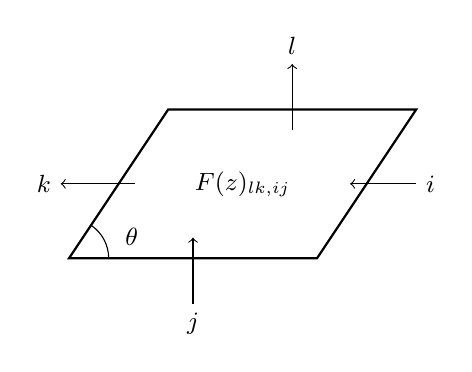
\begin{tikzpicture}[scale=1.05,every node/.style={font=\small}]
 \draw[thick] (0,0)--(3,0)--(4.2,1.8)--(1.2,1.8)--cycle;
 \draw[->] (4.2,.9)--(3.4,.9);
 \draw[->] (.8,.9)--(-.1,.9);
 \draw[->] (1.5,-.55)--(1.5,.25);
 \draw[->] (2.7,1.55)--(2.7,2.35);
 \node[right] at (4.2,.9) {$i$};
 \node[left] at (-.1,.9) {$k$};
 \node[below] at (1.5,-.55) {$j$};
 \node[above] at (2.7,2.35) {$l$};
 \draw (.48,0) arc[start angle=0,end angle=56.31,radius=.48];
 \node at (.76,.26) {$\theta$};
 \node at (2.1,.9) {$F(z)_{lk,ij}$};
\end{tikzpicture}
\caption{Port and tensor order for the checked rhombus matrix.
The horizontal stream enters at the right and leaves at the left;
the vertical stream enters below and leaves above. The arrows specify
the positive spin directions, not a particular allowed path pairing.
The local phase convention is imposed on each pairing separately.}
\label{fig:pv:row}
\end{figure}


For any of the nondegenerate real rhombi used geometrically the allowed pairings can indeed be drawn disjointly with these turns: perturb straight chords between ports by giving them short inward-normal segments at their endpoints (the chord points strictly into the first supporting line's half-plane and out towards the last line, so the two direction changes each have magnitude \(<\pi/2\)). In the two-triangle case the actual honeycomb connections have the same turns.

\begin{lemma}[Local slide and interchange relations]\label{lem:pv:local-relations}
As rational identities, the maps from \(V\) and \(V^{\otimes2}\), respectively,
to \(V^{\otimes3}\) satisfy
\[
 F_{12}(z)F_{23}(Tz)(C\otimes1)=1\otimes C,\qquad
 F_{12}(z)F_{23}(t^2 z)(I\otimes1)=(1\otimes I)F(tz).
\]
The checked matrices also satisfy the Yang--Baxter equation
\[
 F_{12}(y)F_{23}(zy)F_{12}(z)
 =F_{23}(z)F_{12}(zy)F_{23}(y).
\]
\end{lemma}

\begin{proof}
We first prove the slides by projecting onto the three channels. Write
\(m=(1,1+1/\sqrt2,1/\sqrt2)\), \(c=(1/n_0,\sqrt2,2+\sqrt2)\).
The needed small contractions are
\[
 (1\otimes C^t)(C\otimes1)=1,\quad
 (1\otimes C^t)(I\otimes1)=(C^t\otimes1)(1\otimes I)=I^t,\quad
 (1\otimes I)C=(I\otimes1)C,
\]
\[
 (1\otimes I^t)(I\otimes1)/n_0=\sum m_j P_j,\qquad
 1\otimes C-C\otimes1=(2+\sqrt2)(1\otimes I-I\otimes1)I.
\]
All are direct products of the tensors above; e.g. one can use \(C_{ab}=\delta_{a,-b}q^{5a}\) and \(I_{ab,h}=\delta_{h,a+b}J(a,b)\), with \(J(0,0)=1, J(h,-h)=x_*q^{4h},J(h,0)=x_*q^h,J(0,h)=x_*q^{-h}\) for \(h\ne0\) (invalid labels zero); the last identity reads
\[
 \delta_{ah} C_{bc}-C_{ab}\delta_{ch}
 =x_*^{-2}\delta_{a+b+c,h}
 [J(b,c)J(a,b+c)-J(a,b)J(a+b,c)] .
\]
Similarly \((1\otimes I^t)(I\otimes1)=x_*^2(1-CC^t)+II^t\) reduces entrywise at \(a+k=h+c\) to
\[
 J(a,h-a)J(h-a,c)=x_*^2(\delta_{ah}-\delta_{h,-c}q^{5(a+h)})+J(a,k)J(h,c),
\]
using \(q^8=-1,\ q+q^{-1}=x_*^{-1}\).
Consequently \(P_{j,12}(1\otimes C)=c_j P_{j,12}(1\otimes I)I\) (first project onto 0 and 1, then subtract). Project the first slide onto \(P_{j,12}\); the scalar required, relative to its right side, is
\[
 r_j(z)\big[-\delta_{j0}n_0 r_2(Tz)
 -(r_0-r_2)(Tz)/n_0+(r_1-r_2)(Tz)/(n_0 c_j)\big]=1 .
\]
For the second slide sandwich between \(P_{j,12}\) and \(P_k\) on the source. Relative to \(P_{j,12}(1\otimes I)P_k\) the multipliers on the two sides are
\[
 r_j(z)\big[\delta_{j1}r_2(t^2 z)/m_k-\delta_{k1}c_j (r_0-r_2)(t^2 z)+m_k(r_1-r_2)(t^2 z)\big]=r_k(tz)
\]
whenever \(j=1\) or \(k=1\) or \(j=k=2\). The scalar equalities are substitutions of \(a,b\) above: with \(p=t^2\) use the common denominator \((pu-1)(Tu-1)\) for \((r_2,r_0-r_2,r_1-r_2)(u)\), with numerators \((p-u)(T-u),(p-u)(T+1)(u-1),(T-u)(p+1)(u-1)\). At \(u=Tz,pz\) the denominators are \(T(p-z)(T-z),(1+z)(1+tz)\) respectively; \(a(tz)=(p-tz)/(Tz-1)\), \(b(tz)=-(T-tz)/(z+1)\). In the remaining cases the tensor factor vanishes by the contractions. This proves the slides. Inverse and transpose slides follow as well, using unitarity as rational identities.

Explicitly, denoting the three numerators just given by \(D_2,D_0',D_1'\), expansion using \(p^2=-1,\ t=(1+p)/\sqrt2,\ T=(p-1)/\sqrt2\) reads (indices ordered \(0,1,2\))
\[
 \left[-\delta_{j0}n_0 D_2-D'_0/n_0+D'_1/(n_0 c_j)\right](Tz)
 =T\begin{pmatrix}(T-z)(p z-1)\\(p-z)(Tz-1)\\(p z-1)(Tz-1)\end{pmatrix}_j ,
\]
{\small
\[
 \left[\delta_{j1}D_2/m_k-\delta_{k1}c_j D'_0+m_k D'_1\right](pz)
 =
 \begin{pmatrix}
 * & -t(1+tz)(p z-1)&*\\
 -p(1+z)(t-z)&p(p-z)(Tz-1)&T(p-z)(t-z)\\
 * &p(p z-1)(Tz-1)&T(t-z)(p z-1)
 \end{pmatrix}_{j k}
\]
}
where \(*\) entries are not needed.

For Yang--Baxter, clear the denominators and interpolate in \(z\).
For this use of degeneration values in dilute-loop Yang--Baxter
relations, compare~\cite[Section~4]{MorinDuchesnePearce2019}.
Both sides have degree at most four, and for generic \(y\) the five
points
\[
 1,\quad T,\quad t^2,\quad T/y,\quad t^2/y
\]
are distinct. Equality at \(z=1\) is immediate. At \(z=T,t^2\), the
\(z\) factor is \(EE^t\), with \(E=C,I\), respectively; sliding \(E\)
on the left and \(E^t\) on the right gives equality. Here the
reversed-order slide before transposing is the inverse slide at
\(1/(zy)\). The cases \(zy=T,t^2\) follow from the preceding cases
at \((zy,1/y)\) by unitarity. This proves the rational identity.
\end{proof}

\subsection*{Twisted rows and the physical eigenline}

For \(X=(x_1,\ldots,x_N)\) and \(\kappa\ne0\), bring an auxiliary
slot of parameter \(z\) past the sites in their listed order and trace
its output against its input, weighting the identified spin \(h\) by
\(\kappa^h\). This defines the row transfer
\(\mathcal T_\kappa(z;X)\) on \(V^{\otimes N}\). Explicitly, for
input spins \(j_1,\ldots,j_N\) and output spins \(l_1,\ldots,l_N\),
\[
 [\mathcal T_\kappa(z;X)]_{\boldsymbol l,\boldsymbol j}
 =\sum_{i_0,\ldots,i_{N-1}\in\{0,\pm1\}}
 \kappa^{i_0}\prod_{a=1}^N
 F(z/x_a)_{l_a i_a,i_{a-1}j_a},\qquad i_N=i_0.
\]
Thus site order follows the horizontal auxiliary stream, from right to
left in the tile convention of Figure~\ref{fig:pv:row}.

\begin{lemma}[Row relations]\label{lem:pv:row-relations}
At fixed twist, the row transfers commute in their row arguments.
Exchanging adjacent sites by \(F\) intertwines the corresponding rows.
At generic sites, and hence meromorphically,
\[
 \mathcal T_{\kappa}(x_j)\mathcal T_{\kappa}(Tx_j)=1,\qquad
 \mathcal T_{\kappa}(x_j)\mathcal T_{\kappa}(t^2x_j)=\mathcal T_{\kappa}(tx_j).
\]
For adjacent sites \((x,Tx)\), insertion of \(C\) intertwines the row
with the row omitting those sites. For \((x,t^2x)\), insertion of \(I\)
intertwines it with the row having the single site \(tx\). On charge zero,
\(\mathcal T_\kappa(0)=(1+\kappa+\kappa^{-1})1\).
\end{lemma}

\begin{proof}
For commutation, insert a generic invertible crossing of two auxiliary
lines, move it through the sites by Yang--Baxter, and remove it in the
trace; charge conservation preserves the product twist. The same
identity intertwines a site exchange.

For the two row fusion identities, take the indicated auxiliary pair
in that order. The second auxiliary crosses each site first. The slide
preserves its embedded \(C\) or \(I\) subspace throughout, and at the
site \(x_j\) the rank reduction followed by a checked identity sends
the whole auxiliary space into that subspace. The twisted trace is
therefore the fused trace: the product twist on \(C\) is 1, and on
the \(I\) image it is the single twist under the identification.
The inverse slides give the corresponding statements for a pair of
sites. Finally, at row argument zero, triangularity forces the auxiliary
spin to remain constant around the trace. The stated diagonal values
of \(F(0)\), together with charge zero, give
\(1+\kappa+\kappa^{-1}\).
\end{proof}

\begin{lemma}[Physical eigenline]\label{lem:pv:physical-eigenline}
At \(X=(1,\ldots,1)\), \(z=t\), and \(\kappa=\pm i\), powers of
the row transfer converge exponentially to a rank-one projection whose
empty-to-empty entry is 1. In particular, eigenvalue 1 is simple and
all other eigenvalues have modulus less than 1. The same conclusions
hold at the reflected honeycomb point \(z=t^2\).

Near either set of physical sites and twist, the rows have a common
analytic eigenline of charge zero. Its eigenvalue is rational in the
row argument and analytic in the other data near regular arguments.
At \(\kappa=\pm i\) this row eigenvalue is identically 1.
\end{lemma}

\begin{proof}
The empty basis tensor has all spins zero. At the homogeneous point,
closed loops cancel after orientation summation: contractible loops
have turns \(\pm2\pi\), with trace twist net 1, while simple essential
loops have winding \(\pm1\), trace twist \(\kappa^{\pm1}\), and total
turn zero. The latter total turn follows from the exterior-angle sum
on the annular region between the curve and a distant parallel geodesic,
which is zero by triangulation and Euler's formula. The winding assertion
also follows by identifying the cylinder with a punctured plane. Gauge
factors telescope, so only prescribed boundary-to-boundary arcs remain.

At least one crossing arc gives an exponentially small contribution
by the finite-width cylinder bounds in Lemma~\ref{lem:pv:cylinder-decay}.
With no crossing arc,
the systems along the two cuts factor in the limit into half-cylinder
amplitudes. Their error is exponentially small, since a system preventing
factorization must reach halfway across the cylinder height. There are
only finitely many boundary pairings and orientations, and dropping
mutual avoidance bounds each of them by products of arc weights. This
gives the rank-one limit. Its empty-to-empty entry is 1 because every
nonempty closed system cancels already at finite height. Reflection
gives the same argument at the other honeycomb realization.

Finite-dimensional perturbation of \(\mathcal T_\kappa(t)\) now gives
a simple analytic eigenline near the physical data. Commutation makes
it a common eigenline, and charge conservation keeps it in charge zero.
For fixed sites and twist its row eigenvalue is rational in \(z\).

To identify this eigenvalue at \(\kappa=\pm i\), first take real nearby
spectral angles \(z=e^{2iu},x_j=e^{2i\alpha_j}\). Lay the rows using
unit rhombus side vectors with directions \(8u/3\) and bottom vectors
with directions \(8\alpha_j/3\). The slightly zigzag spatial boundary
repeats by translation and projects monotonically onto the direction
perpendicular to the row side vector, so the rows do not overlap.
Loop turns and twists still cancel. The gauge factors telescope because
\(v=u-\alpha_j\) and \(i-k=l-j_{\rm spin}\) at every crossing: the
\(u\) term sums along auxiliary strands and the site-angle term along
site strands. Hence every empty-to-empty power remains 1.

Analyticity extends this equality to complex nearby data. With \(z\)
also near \(t\), all other eigenvalues remain strictly inside the unit
disk and the empty entry of the near-1 projection is nonzero. The
constant power entry therefore forces the distinguished eigenvalue
and that projection entry to equal 1. Rational continuation in \(z\)
finishes the proof.
\end{proof}

\subsection{Polynomial vacuum}\label{c01-c1-polynomial-vacuum}

Polynomial exchange and fusion constructions occur in the dense and dilute $O(1)$ models~\cite{DiFrancescoZinnJustin2005,GarbaliNienhuis2017Ground,GarbaliNienhuis2017Sum}. We construct the present normalized vacuum directly by polynomial interpolation and determine its empty component. Its Pfaffian formula supplies the denominator of the polygon observable.

\begin{proposition}[Polynomial vacuum]\label{prop:pv:vacuum}
Use twist \(\zeta=t^2=i\). Let \(\rho X=(x_N,x_1,\ldots,x_{N-1})\), and \(\Pi_\kappa\) the corresponding rotation of spin slots with factor \(\kappa^{h_N}\) from the last (now first) spin. We construct a charge-zero vector polynomial \(\Psi_N(X)\) with
\[
 F_{i,i+1}(x_i/x_{i+1})\Psi(X)=\Psi(s_i X),\qquad
 \Pi_\zeta\Psi(X)=\Psi(\rho X)
\]
(\(s_i\) adjacent transposition), homogeneous of degree \(\binom N2\),
with degree at most \(N-1\) in each variable. For a spin component
\(\Psi_{N,\boldsymbol h}\), the refined bounds are
\[
 h_j=+1\ \Longrightarrow\ \deg_{x_j}\Psi_{N,\boldsymbol h}\le N-2,
 \qquad
 h_j=-1\ \Longrightarrow\ x_j\mid\Psi_{N,\boldsymbol h}.
\]
It has the adjacent-pair reduction
\[
 \Psi_N(\ldots,a,Ta,\ldots)=s_C(a;Y)\ \iota_C \Psi_{N-2}(Y),
 \qquad
 s_C(a;Y)=(1+T)a\prod_{x\in Y}(x-t^5a)(x-t^6a),
\]
where \(Y\) is the remaining list and \(\iota_C\) inserts a \(C\) tensor in the indicated positions; and at last parameter zero its projection onto last spin zero is \((\prod_{j<N}x_j)\Psi_{N-1}\).

\end{proposition}

\begin{proof}
We induct on \(N\). The construction has five steps: prescribe cup
values and interpolate; prove the spectator degree bounds; propagate
all cup reductions; prove the last exchange; and prove cyclicity.
The refined bounds are the reason the last two discrepancies vanish.

The initial vectors are \(\Psi_0=1\) and \(\Psi_{1,0}=1\), with
the other size-one components zero. At sizes two and three, the empty
components are
\[
 S_2(a,b)=a+b,\qquad
 S_3(a,b,c)=\sum_{i\ne j}x_i^2x_j+2\sqrt2\,abc,
 \quad (x_1,x_2,x_3)=(a,b,c).
\]
At size three, components with first pair \((h,-h)\) and last spin
zero are
\[
\begin{gathered}
 f_h(a,b;c)=2\sin\lambda\,t^h L_h(a,b)P(a,b;c),\\
 L_+(a,b)=b,\quad L_-(a,b)=a,\qquad
 P(a,b;c)=(c+ta)(c+b/t).
\end{gathered}
\]
At size two omit \(P\). Cyclicity specifies the remaining components.
We verify these initial cases at the end of the proof.

\paragraph{Cup values and interpolation.}
Assume the proposition at lower sizes and let \(N\ge4\). Set
\(Y_i=(x_1,\ldots,\widehat{x_i},\ldots,x_{N-1})\). To prescribe
the value at \(x_N=Tx_i\), insert \(C\) in the parameter list
\((x_1,\ldots,x_i,Tx_i,x_{i+1},\ldots,x_{N-1})\), then carry
its second slot to the end. With rightmost factor acting first, this is
\[
 V_i=s_C(x_i;Y_i)
 F_{N-1,N}(Tx_i/x_{N-1})\cdots
 F_{i+1,i+2}(Tx_i/x_{i+1})\,
 \iota_{C,i}\Psi_{N-2}(Y_i).
\]
The product is empty when \(i=N-1\). At the crossing with \(x_d\),
the two denominator factors are proportional to
\((x_d-t^5x_i)(x_d-t^6x_i)\), already present in \(s_C\).
Thus each \(V_i\) is polynomial.

These prescriptions are covariant under exchanges among the first
\(N-1\) sites, carrying the marked value with its site. An exchange
away from the mark uses lower-size exchange and Yang--Baxter. At the
mark, the local identity is the cup slide
\[
 F_{12}(a/b)F_{23}(Ta/b)(C\otimes1)=1\otimes C:
\]
it moves the cup based at \(a\) past its neighbor \(b\), without
changing \(s_C(a;Y)\). The inverse slide handles the opposite order;
Yang--Baxter moves a distant exchange into this local configuration.

For last spin plus, interpolate the \(N-1\) values with degree
\(N-2\). For last spin minus, interpolate the value divided by
\(x_N\) with that degree. For last spin zero, add the prescribed
zero node and use degree \(N-1\). More explicitly, put
\[
 \ell_i=\prod_{\substack{d<N\\d\ne i}}
 \frac{x_N-Tx_d}{T(x_i-x_d)}.
\]
The multiplier of \(V_i\) is \(\ell_i\) for last spin plus and
\(x_N\ell_i/(Tx_i)\) otherwise. In last spin zero add
\(\prod_{d<N}(x_d-x_N/T)\Psi_{N-1}\).

The apparent poles at \(x_i=x_d\) cancel: coincident nodes have
identical prescriptions by exchange covariance. Indeed exchanging
equal parameters through intervening slots is the identity by
unitarity, initially at generic other parameters. The only other
possible poles, the simple poles at \(x_i=0\), cancel because
\(x_i\mid V_i\). The result is polynomial, with total degree
\(\binom N2\) by homogeneity. Interpolation also proves all exchanges
among the first \(N-1\) sites.

\paragraph{Spectator bounds.}
Fix \(j<N\). For \(V_i\) with \(i\ne j\), the lower-size bound
and the quadratic factor in \(s_C\) give degree at most \(N-1\)
in \(x_j\). If slot \(j\) is crossed, then as \(x_j\to\infty\)
the crossing argument tends to zero. Its leading output spin at that
site is no larger than the input spin, so an output plus spin retains
the lower-size degree loss. At \(x_j=0\) the opposite triangularity
preserves the required minus-spin zero. The Lagrange multipliers are
bounded at both ends. The extra zero-node term has the same bounds
directly from size \(N-1\).

The term \(V_j\) has larger raw degree because \(x_j\) is the cup
parameter. Its orders and the two possible multipliers are
\[
\begin{array}{c|cc}
 &x_j\to\infty&x_j\to0\\ \hline
 V_j&O(x_j^{2N-3})&O(x_j)\\
 \ell_j&O(x_j^{-(N-2)})&O(1)\\
 x_N\ell_j/(Tx_j)&O(x_j^{-(N-1)})&O(x_j^{-1})
\end{array}
\]
These give all unrefined bounds. There are only two extra cases to
check. At infinity, if both site \(j\) and the final site have spin
plus, the carried cup spin starts minus and cannot increase under
the leading \(F(\infty)\) transport. The leading coefficient is
therefore zero, supplying one more degree of decay. At zero, if
site \(j\) has spin minus and the final spin is not plus, the carried
spin starts plus and cannot decrease under \(F(0)\). Its leading
term again vanishes, compensating for the possible simple pole in
the multiplier. This proves both refined bounds at every spectator.

\paragraph{Compatibility of cup reductions.}
To prove the adjacent reduction at \(x_{j+1}=Tx_j\) among the first
\(N-1\) sites, check it at the last-variable interpolation nodes.
Disjoint cup specializations commute by the slides and lower-size
exchange and reduction. Their scalar factors commute as well: for
two cup parameters \(a,d\), their cross factor is
\[
 \prod_{y\in\{d,Td\}}(y-t^5a)(y-t^6a)
 =T^2\prod_{r\in\{t^2,T,t^5,t^6\}}(d-ra).
\]
The four roots occur in reciprocal pairs and have product one, so
this expression is unchanged on exchanging \(a,d\).

At the overlapping node \(x_N=Tx_{j+1}\), both sides vanish: one
has the \(x_N\) spectator factor, and the other the \(x_j\) factor
in \(V_{j+1}\), whose slot is not crossed. At
\(x_N=Tx_j=x_{j+1}\), the first crossing in \(V_j\) is a checked
identity. It leaves the required cup and the lower-size exchange
transport of the remaining spectator. At the zero node in spin zero,
the scalar factors agree because \(t^{5+6}=T\). Interpolation proves
the adjacent reduction. Together with the exchanges already proved,
this gives every specialization \(x_k=Tx_i\), \(i<k\), with the
stated transport for nonadjacent slots.

\paragraph{The last exchange.}
Clear denominators in the remaining exchange discrepancy:
\[
 \mathcal D=(t^2x_{N-1}-x_N)(Tx_{N-1}-x_N)
 \big[F_{N-1,N}(x_{N-1}/x_N)\Psi(X)-\Psi(s_{N-1}X)\big].
\]
It vanishes on every cup hyperplane \(x_k=Tx_i\), \(i<k\), except
possibly the pair \((N-1,N)\). For an unaffected pair this is lower-size
exchange after cup reduction. When the second member is exchanged,
the cup transports acquire precisely that exchange or its inverse.
Consequently \(\mathcal D=Q E\), where
\[
 Q=\prod_{\substack{i<k\\(i,k)\ne(N-1,N)}}(x_k-Tx_i).
\]
Each spectator \(x_j\), \(j\le N-2\), occurs in exactly \(N-1\)
factors of \(Q\), exhausting the degree bound on \(\mathcal D\).
Thus \(E\) is independent of every spectator. The plus-spin degree
loss and minus-spin zero force all those spectator spins to be zero.
For adjacent spectators, however,
\(Q(s_jX)/Q(X)=b(x_j/x_{j+1})\). Their exchange equation therefore
forces \(F E=b E\), so their pair lies in channel 1. A nonzero pure
\(|00\rangle\) does not belong to \(\operatorname{im}I\), and there
are at least two spectators. Hence \(E=0\), proving full exchange.

\paragraph{Cyclicity.}
Lower-size cyclicity and the cup reductions show that
\[
 \Pi_\zeta^{-1}\Psi(\rho X)-\Psi(X)
 =\prod_{i<k\le N-1}(x_k-Tx_i)\,E(X).
\]
The specialized pair never straddles the rotation seam. The quotient
has degree at most one in each of its first \(N-1\) variables, so write
\[
 E(X)=\sum_{\epsilon\in\{0,1\}^{N-1}}
 x_1^{\epsilon_1}\cdots x_{N-1}^{\epsilon_{N-1}}
 E_\epsilon(x_N).
\]
By the refined bounds, bit zero permits spins \(0,+\) and bit one
permits spins \(0,-\). Exchange of adjacent variables among these
first \(N-1\) acts on \(E\) by
\[
 E(s_jX)=\big(aP_2+P_1+(a/b)P_0\big)_{j,j+1}E(X),
 \qquad a=a(x_j/x_{j+1}),\quad b=b(x_j/x_{j+1}).
\]

\begin{claim}
A tensor polynomial multiaffine in at least three consecutive variables,
with the bit-dependent spin support and exchange relation just stated,
is zero.
\end{claim}

\begin{proof}[Proof of the claim]
For an adjacent pair, the two uncanceled denominator factors of
\(a/b\), namely \(t^2x_j-x_{j+1}\) and \(Tx_{j+1}-x_j\),
must divide \(P_0E\). Their product has degree two in each
variable, whereas \(P_0E\) is multiaffine. Hence \(P_0E=0\).
The channel-1 part is symmetric. The channel-2 part is divisible by
\(x_{j+1}-t^2x_j\), with quotient independent of those two variables.
Consequently, with all other bits fixed, the adjacent coefficients obey
\[
 E_{10}=(P_1-t^2P_2)E_{01}.
\]
This operator is invertible on channels 1 and 2.

It suffices, therefore, to kill coefficients with sorted bits. Equal
adjacent bits require channel 1. With the permitted spins, their pair
must be proportional to \(I_+\) for 00 or \(I_-\) for 11.
Three equal bits are impossible: a first pair proportional to \(I_h\)
and either third spin \(0,h\) would produce a forbidden second pair
\(00\) or \(hh\). For 0011 the four slots must factor as
\(I_+\otimes I_-\). Their middle cup contraction is zero because
\(P_0E=0\), but fixing the end spins \(+,-\) makes that contraction
nonzero unless the coefficient vanishes. For 001, fix the first spin
plus and then zero. The cup contraction on the last two excludes
third spin zero and then minus, killing the coefficient through the
first-pair combination. The argument for 011 is the same with the
ends reversed. These exhaust sorted binary strings of length at least
three: either some bit occurs three times, both occur at least twice,
or the string is 001 or 011. This proves the claim.
\end{proof}

Apply the claim to the first \(N-1\) variables. Since \(N\ge4\),
the cyclic discrepancy vanishes.

\paragraph{Verification of the initial cases.}
The size-two and size-three formulas above meet the cup, zero, and
degree conditions directly. To check the first exchange by the explicit
blocks of \(F\), write \(S\) for the corresponding empty polynomial
and substitute \(e^{2iv}=a/b\) in the local weights. The scalar
identities used are
\[
\begin{aligned}
 P(b,a;c)&=w_1 P(a,b;c)+u_2 S/(2\sin\lambda\sqrt{ab}),\\
 P(c,b;a)&=u_1\sqrt{a/b}\,P(c,a;b)+o P(b,c;a),\\
 P(a,c;b)&=oP(c,a;b)+u_1\sqrt{b/a}\,P(b,c;a).
\end{aligned}
\]
(with square-root branch corresponding to \(v\)); at size 2 only the first, with the two \(P\)'s replaced by 1. For the first identities compare coefficients, using
\[
\begin{aligned}
 1-w_1&=u_2\cos v/\sin\lambda,\\
 \cos(2\lambda-v)-w_1\cos(2\lambda+v)
 &=(u_2/(2\sin\lambda))(\cos(2v)+\sqrt2).
\end{aligned}
\]
For the other two use \(u_1 e^{iv}+o/t=u_1 e^{-iv}+ot=\sin(3\lambda-v)/\sin(3\lambda+v)=(b+t a)/(a+t b)\). The \(w_2\) terms on the occupied pair cancel since \(t^2=i\); likewise the two contributions to the change of the empty component. Remaining exchanges follow by rotation not wrapping the pair. This verifies the bases, and finishes the construction.

\end{proof}

\subsubsection*{The physical normalization and its empty component}

The polynomial vector now determines the physical common eigenline.
We identify its empty component, which will be the denominator of the
separator pairing.

First,
\[
 \mathcal T_\zeta(z;X)\Psi(X)=\Psi(X).
\]
At \(z=x_N\) the last crossing is a checked identity. The row is
\(\Pi_\zeta\) followed by transport of its first parameter to the
end, so the exchange and cyclic equations prove the equality there.
Exchange gives it at all \(x_j\), row fusion/inversion gives it at
all \(Tx_j\), and triangularity gives it at zero. After clearing row
denominators, the degree is at most \(2N\). The \(2N+1\) generic
points \(0,x_1,\ldots,x_N,Tx_1,\ldots,Tx_N\) therefore suffice.

Similarly \(\Psi(X^{-1})^t\), with \(X^{-1}\) the entrywise reciprocal
list, is a left eigenvector of eigenvalue 1 for twist \(\zeta^{-1}\).
At \(z=x_N\), reverse transport through the symmetric crossings has
exactly the exchange arguments that move the last reciprocal parameter
to the first; the final rotation cancels because
\(\Pi_{\zeta^{-1}}^t\Pi_\zeta=1\). The other interpolation points
follow as above by inverse and transpose exchanges.

Let \(S_N\) be the empty component, which is not identically zero by
cup reduction, and put \(\Omega=\Psi/S_N\). For generic sites near
homogeneity, Lemma~\ref{lem:pv:physical-eigenline} identifies \(\Omega\)
with the lower half-cylinder state obtained from empty input far below,
normalized to have empty component 1. Its reciprocal transpose is the
analogously normalized left state at twist \(\zeta^{-1}\).

The symmetry of \(S_N\) requires this geometric normalization: it does
not follow just by taking the empty component of exchange, since that
component mixes with occupied pairs. Take real nearby angles with
\(\alpha_i>\alpha_{i+1}\) in the earlier embedding. From left to
right the upper boundary has site steps of directions
\(8\alpha_{i+1}/3,8\alpha_i/3\). Adding the rhombus above those
steps exchanges their order, entering from right and bottom with
parameters \(x_i,x_{i+1}\), without crossing the twist seam.
With empty final output, all gauge factors telescope and all loops
cancel even at finite height. The added crossing therefore takes one
normalized half-cylinder state to the other with no scalar factor.
Comparing with polynomial exchange gives \(S_N(s_iX)=S_N(X)\).
This extends polynomially from the open set of real angles.

\begin{proposition}[Empty component]\label{prop:pv:empty-component}
Put \(D(a,b)=a^2+\sqrt2 ab+b^2\) and
\(K(a,b)=(a^2-b^2)/D(a,b)\). The symmetric empty component is
\[
 S_N(X)=\prod_{i<j}\frac{D(x_i,x_j)}{x_i-x_j}\ {\rm Pf}[K(x_i,x_j)]
\]
where for odd size an extra last Pfaffian index has
\(K_{i,N+1}=1\), \(i\le N\), corresponding to parameter zero.
It satisfies
\[
 S_N(X^{-1})=\frac{S_N(X)}{\prod_i x_i^{N-1}}
\]
and the second fusion identity
\[
 S_N(a,t^2a,Y)=\sqrt2\,t a\prod_{y\in Y}(y-t^5 a)\ S_{N-1}(ta,Y).
\]
\end{proposition}

\begin{proof}
The displayed Pfaffian expression is a symmetric polynomial of the
required degrees. Its cleared numerator is alternating, so the
Vandermonde denominators cancel; the remaining possible poles cancel
against the factors \(D\). The bounded kernel at infinity gives the
one-site degree bound. At a first pair \((a,Ta)\), only its own
Pfaffian pairing survives and gives \(s_C S_{N-2}\). A last zero
parameter gives the zero-node prescription; if a dummy zero is present,
only their mutual pairing remains. Symmetry and interpolation identify
the expression with \(S_N\). Inversion of all parameters gives the
reciprocity formula. The zero-node identity and reciprocity also give
the leading-coefficient identity
\[
 [x_N^{N-1}]S_N(X)=S_{N-1}(x_1,\ldots,x_{N-1}).
\]

For the second fusion identity, compare its two sides in a spectator
variable. Cup reduction at another spectator is compatible on both
sides because
\[
 (a-t^5d)(a-t^6d)(t^2a-t^5d)(t^2a-t^6d)
 =(d-t^5a)(Td-t^5a)(ta-t^5d)(ta-t^6d)
\]
for a spectator pair \(d,Td\). Each of the other \(N-3\) spectators
therefore gives two roots, at ratios \(T\) and \(T^{-1}\), by symmetry.
The zero-node identity gives one more root. The leading-coefficient
identity makes the top degrees agree, lowering the degree of the
difference to at most \(N-2\). Thus its \(2(N-3)+1\) roots suffice
for \(N\ge4\); sizes two and three follow from the initial formulas.
\end{proof}

\begin{corollary}[Normalized reductions]\label{cor:pv:normalized-reductions}
At generic parameters, the normalized states reduce by insertion of
\(C\) at adjacent sites \((a,Ta)\), and by insertion of \(I\) at
\((a,t^2a)\), replacing those sites by the single site \(ta\).
When one parameter tends to zero or infinity, the spin-zero component
at that slot tends to the reduced \(\Omega\), with scalar factor one.
\end{corollary}

\begin{proof}
The cup assertion follows from the identical scalar reductions of
\(\Psi\) and \(S_N\). At \((a,t^2a)\), the pole in the exchange
equation forces channel 1. On that subspace the row intertwines the
reduced row by Lemma~\ref{lem:pv:row-relations}. Its eigenvalue-1
space is a unique line for generic reduced sites: it is one-dimensional
at homogeneous sites, and rational matrix minors preserve that property
generically. The reduced site \(ta\) can be generic. Empty-component
normalization fixes the insertion scalar to be one.

At zero, use rotation and the zero-node prescription. At infinity,
the limit exists generically by the degree bounds and has no plus
spin at the extreme slot. After projection to spin zero, triangularity
at crossing argument zero makes the transfer the reduced row.
Uniqueness again identifies the limit, and the nonzero generic leading
coefficient of \(S_N\) fixes its normalization.
\end{proof}

\section{The balanced puncture observable}\label{c01-c1-the-balanced-puncture-observable}

A contraction of the two vacua will count polygons separating two specified cylinder faces. We first establish that positive interpretation and then the interpolation data that characterize the contraction.

Divide the ordered sites into a first block A of size \(n\) and remaining block B of size \(m=N-n\). Define
\[
 X_{n,m}(X;\kappa)=\Omega(X^{-1})^t D_{\kappa/\zeta}^{\rm A}\,\Omega(X)
\]
where the diagonal multiplies by \((\kappa/\zeta)^{\sum_{j\in{\rm A}}h_j}\), for \(\kappa\ne0\).
\begin{samepage}
\begin{proposition}[Physical separator pairing]\label{prop:pv:physical-pairing}
For two homogeneous blocks of equal size $n$,
\[
 X_{n,n}(1,\ldots,1;\kappa)=F_n(\kappa+\kappa^{-1}).
\]
Here the left side is the bilinear vacuum contraction just defined and the right side is the positive polygon polynomial from Section~\ref{sec:pv:introduction}.
\end{proposition}
\end{samepage}

\begin{proof}
Work first at finite height with homogeneous sites. If \(|0\rangle\)
is the empty tensor, the lower and upper boundary states are
\[
 |u_H\rangle=\mathcal T_\zeta(t)^H|0\rangle,
 \qquad
 \langle v_H|=\langle0|\mathcal T_{\zeta^{-1}}(t)^H.
\]
Every empty-to-empty entry is 1 by loop cancellation.
Lemma~\ref{lem:pv:physical-eigenline} and the normalized left and right
eigenvectors therefore give
\[
 |u_H\rangle\longrightarrow\Omega(1,\ldots,1),\qquad
 \langle v_H|\longrightarrow\Omega(1,\ldots,1)^t.
\]
The upper state is obtained by rows between the gluing cut and an empty
upper boundary; its twist is \(\zeta^{-1}\). This identifies the
reciprocal left eigenvector geometrically by the rank-one limit.
At nonsingular physical data we always use these analytic states,
including when their rational formulas are evaluated by a limit.

The finite contraction \(\langle v_H|D_{\kappa/\zeta}^{\rm A}|u_H\rangle\)
glues matching occupied ports to make disjoint polygons. Internal gauge
factors telescope under this gluing. It has three
directed seams: from the lower boundary to \(f\), with weight
\(\zeta\); from \(f\) to the upper boundary, with weight
\(\zeta^{-1}\); and from the block-division face \(f'\) to \(f\)
along block A, with weight \(\kappa/\zeta\). See
Figure~\ref{fig:pv:seams}. Positive crossing is toward the left of a
directed seam. For an oriented simple polygon, let \(L(a)\) indicate
whether \(a\) lies on its left. The signed crossing number of a seam
\(a\to b\) is \(L(a)-L(b)\), so its three seam factors multiply to
\[
 \zeta^{L(-\infty)-L(f)}
 \zeta^{-L(f)+L(+\infty)}
 (\kappa/\zeta)^{L(f')-L(f)}.
\]
Here the two end indicators may be taken at the empty finite boundaries.
For a contractible polygon oriented with interior left, the turn factor
is \(i=\zeta\) and both end indicators are zero. For an essential
polygon oriented with upper end left, the turn factor is 1 and the
end indicators are zero and one. In both cases the total factor is
\[
 \zeta^{1-L(f)-L(f')}\kappa^{L(f')-L(f)}.
\]
The reverse orientation contributes its inverse. Equal indicators
therefore give \(\zeta+\zeta^{-1}=0\), whereas unequal indicators
give \(\eta=\kappa+\kappa^{-1}\). Exactly the separating polygons
survive, with their critical vertex weights.

At each finite height the contraction is consequently a polynomial
in \(\eta\) with nonnegative coefficients. Its degree is at most
\(n\), since every separating polygon uses a distinct port of block A.
The coefficients increase as the height grows. At any fixed positive
\(\eta\), convergence of the two boundary states bounds the
contractions, and hence bounds every coefficient. Their finite limits
are exactly the infinite-cylinder polygon sums. Passing to the limit
coefficientwise proves the claimed identity for every \(\kappa\ne0\).

\end{proof}

\begin{figure}[tb]
\centering
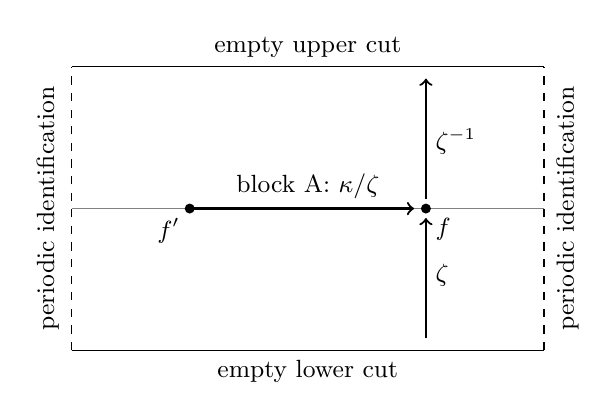
\begin{tikzpicture}[x=1cm,y=1cm,every node/.style={font=\small}]
 \draw[dashed] (-3,-1.8)--(-3,1.8);
 \draw[dashed] (3,-1.8)--(3,1.8);
 \draw (-3,-1.8)--(3,-1.8);
 \draw (-3,1.8)--(3,1.8);
 \draw[gray] (-3,0)--(3,0);
 \draw[thick,->] (1.5,-1.65)--(1.5,-.12);
 \draw[thick,->] (1.5,.12)--(1.5,1.65);
 \draw[thick,->] (-1.5,0)--(1.35,0);
 \fill (1.5,0) circle (1.8pt);
 \fill (-1.5,0) circle (1.8pt);
 \node[below right] at (1.5,0) {$f$};
 \node[below left] at (-1.5,0) {$f'$};
 \node[right] at (1.5,-.85) {$\zeta$};
 \node[right] at (1.5,.85) {$\zeta^{-1}$};
 \node[above] at (0,0) {block A: $\kappa/\zeta$};
 \node[above] at (0,1.8) {empty upper cut};
 \node[below] at (0,-1.8) {empty lower cut};
 \node[rotate=90] at (-3.3,0) {periodic identification};
 \node[rotate=90] at (3.3,0) {periodic identification};
\end{tikzpicture}
\caption{The finite cylinder, cut open along the two identified dashed
sides. The middle line is the gluing cut; the arrows are directed twist
seams, not polygon segments. Block A follows the site order from $f$
toward $f'$, while its seam is directed from $f'$ to $f$. The empty
upper and lower cuts recede to the cylinder ends in the limit.}
\label{fig:pv:seams}
\end{figure}

\begin{remark}[Comparison of the scalar and physical pairings]\label{rem:pv:scalar-comparison}
For $N=2n$, reversing both the numerator and Vandermonde conventions
leaves the empty polynomial unchanged:
\[
 S_{2n}(X)=\prod_{i<j}\frac{D(x_i,x_j)}{x_j-x_i}
 \operatorname{Pf}\!\left[\frac{x_j^2-x_i^2}{D(x_i,x_j)}\right].
\]
The prefactor changes by $(-1)^{n(2n-1)}$ and the Pfaffian by
$(-1)^n$, whose product is one. This is exactly the scalar convention
of~\cite[Section~5.2]{DiskTransfer2026}.

Multiplying our lattice coordinates by $\sqrt3$ gives honeycomb edge
length one. It preserves polygon vertices, critical weights, and which
polygons separate the marks, and therefore preserves $F_n$ on the
rescaled cylinder.
For $n\ge3$, the disk construction in
\cite[Section~5.3]{DiskTransfer2026} identifies its physical pairing
with this same polygon sum. These comparisons concern the scalar
polynomial and the physical observable; the inhomogeneous vectors and
their denominator estimates remain separate constructions.
\end{remark}

\subsection{Interpolation of the contraction}

The following characterization will identify the finite color formula
in Section~\ref{c01-c1-color-formula-and-small-cycle-gas}. It applies
at generic parameters; it does not assert that \(S_N\) is nonzero
at every complex specialization. In the displays below we separate
the site lists of the two blocks by a semicolon.

\begin{proposition}[Interpolation of the pairing]\label{prop:pv:pairing-interpolation}
Fix \(\kappa\ne0\) and put \(\eta=\kappa+\kappa^{-1}\).
The family \(X_{n,m}\) is uniquely determined among rational functions
by the following properties. It is symmetric separately in its two
blocks, and \(S_N^2X_{n,m}\) is polynomial of degree at most
\(2(N-1)\) in each site, where \(N=n+m\). Within block A its
reductions are
\[
\begin{aligned}
 X_{n,m}(a,Ta,A';B)&=X_{n-2,m}(A';B),\\
 X_{n,m}(a,t^2a,A';B)&=X_{n-1,m}(ta,A';B),\\
 \lim_{a\to0\text{ or }\infty}X_{n,m}(a,A';B)
 &=X_{n-1,m}(A';B),
\end{aligned}
\]
The pair reductions require \(n\ge2\), and the extreme reduction
requires \(n\ge1\); the analogous rules hold in block B with \(m\)
in place of \(n\). The initial value is
\(X_{0,0}=1\), and at every balanced size \(n=m>0\),
\[
 X_{n,n}(a_1,\ldots,a_n;Ta_n,\ldots,Ta_1)=(1+\eta)^n.
\]
\end{proposition}

\begin{proof}
Separate block symmetry follows from exchange and its inverse,
transpose symmetry of \(F\), and charge conservation. Reciprocity
of \(S_N\) shows that \(S_N^2X_{n,m}\) is the contraction of two
polynomial vectors, each of degree at most \(N-1\) per site; this
gives the degree bound.

For the extreme reductions, the complementary vanishing of nonzero
spins on the two sides leaves only the spin-zero limit in
Corollary~\ref{cor:pv:normalized-reductions}. At an adjacent cup the
right vector inserts \(C\). In the reciprocal vector, the projection
onto the same channel inserts \(C/r_0(T)\): exchanging its reversed
pair into cup order acts by \(F(T)=r_0(T)P_0\). Contraction cancels
the scalar because \(C^tC=r_0(T)=-n_0\), and the block twist
preserves the pair. At the other fusion, use
\(F(t^2)=n_0P_1\) and \(I^tI=n_0\,1\) in the same way.
The block twist on the image of \(I\) is the single-site twist.
These are rational identities on the generic domain.

At the balanced specialization, successive nested cups in the right
vector force spins \(h\) on A with opposite mates in B and amplitudes
\(\prod q^{5h}\). Rotate B to the beginning in the reciprocal vector.
Its cups now face the other way, so in the original order its amplitudes
are \(\prod\zeta^h q^{-5h}\). Together with the block insertion,
each pair contributes \(\sum_{h=0,\pm1}\kappa^h=1+\eta\).
This gives the last specialization.

For uniqueness, suppose two families agree at smaller sizes, and let
\(A(X)\) be their difference at \((n,m)\), multiplied by \(S_N^2\).
The zero and infinity reductions give respectively
\(x_i\mid A\) and \(\deg_{x_i}A\le2N-3\) at each site. The
cup and second fusion, in both orders, give four factors for each
intra-block pair. Thus
\[
 Q(X)=\left(\prod_{i=1}^Nx_i\right)
 \prod_{P\in\{\mathrm A,\mathrm B\}}
 \prod_{\substack{i<j\\i,j\in P}}
 \prod_{d\in\{2,3,5,6\}}(x_j-t^d x_i)
 \quad\hbox{divides }A(X).
\]
In a site of A this divisor has degree \(4(n-1)+1\), leaving
\[
 \deg_{x_i}(A/Q)\le2N-3-[4(n-1)+1]=2(m-n).
\]
In a site of B the remaining degree is at most \(2(n-m)\).
An unbalanced difference is therefore zero. In a balanced case the
quotient is a scalar; the nested-cup specialization fixes it to zero,
since it is generically off the zero sets of both \(Q\) and \(S_N\).
Induction from \(X_{0,0}=1\) completes uniqueness.
\end{proof}

\section{The boundary exponent}\label{c01-c1-the-boundary-exponent}

We now determine the strip mass needed to normalize chordal walks. The row derivative reduces this problem to a positive polynomial-kernel estimate and a comparison of geometric tails.

\begin{proposition}[Boundary exponent]\label{prop:pv:boundary}
For critical bridges across $h$ layers from a fixed bottom port to all top ports, $b_h=h^{-1/4+o(1)}$. The half-plane arch mass to the right is $1/(2\cos(3\pi/8))$; its height and diameter tails both have exponent $-1/4$.
\end{proposition}

The proof has three stages. A row derivative gives an exact excluded-arch mass. A positive polynomial-kernel estimate gives its power, and a two-direction flux comparison changes the cylinder exclusion into a strip-height tail. This argument uses the row relations and physical eigenline from Lemmas~\ref{lem:pv:row-relations} and~\ref{lem:pv:physical-eigenline}, independently of the polynomial vacuum and separator pairing.

\subsection{Row susceptibility at infinity}\label{c01-c1-row-susceptibility-at-infinity}

Use even widths \(N=2m\). Let \(G_N\) be the half-plane mass, from a fixed bottom port, of arches with positive endpoint displacement \(0<d<N\) whose projections to the cylinder of period \(N\) are simple. The strip flux bound gives \(G_N\le1/(2\cos(3\lambda))\). We will express this deficit through one Taylor coefficient of a row eigenvalue.

For the common eigenline near twist \(\kappa=i\), differentiate its row eigenvalue in \(\eta=\kappa+\kappa^{-1}\) at zero. Call the answer in homogeneous data \(H(\theta)\), with \(z=e^{2iv},\ \theta=2v-3\lambda\); we also write \(H(z)\) when using the transfer argument. It tends to 1 as \(z\to0,\infty\) by triangularity. It is even: at real \(v\) near \(\lambda\), empty-to-empty powers agree with those at \(3\lambda-v\) by reflection of the unoriented loop sum (\(u_1,u_2\) and \(w_1,w_2\) interchange). The simple eigenvalue strictly dominates nearby at both parameters, so they agree there on that eigenvalue and then by continuation. Its denominator may be taken to be \((\cos\lambda+\cos\theta)^N\).

Before making sites homogeneous, transfer fusion gives for the derivative as a function of transfer argument \(z\) both relations
\[
 H(z)+H(Tz)=0,\qquad H(z)+H(t^2z)-H(tz)=0
\]
at every \(z=x_j\) (base eigenvalue 1). Thus the relations have zero jets of orders below \(N\) at the common site 1, by analyticity in sites and coalescence (all the denominators here regular locally; e.g. divide by \(\prod(z-x_j)\) for nearby distinct sites and bound inside a small circle). In \(\theta\) notation the site and its shifts \(t,t^2,T\) correspond to \(-3\lambda,-\lambda,\lambda,3\lambda\). By evenness the jets are
\[
 H^{(2j)}(3\lambda)=0,\qquad
 H^{(2j+1)}(3\lambda)=2H^{(2j+1)}(\lambda)\quad(0\le j<m).
\]

Represent the cosine-rational function as
\[
 H(\theta)=1+\int_{\mathbb R} e^{\theta p}
 \frac{\sinh(\lambda p)U(p^2)+p\cosh(\lambda p)V(p^2)}{\sinh(\pi p)}\,dp
\]
with polynomials of degrees below \(m\). Indeed, near the real angles used here,
\[
 \int_{\mathbb R}\frac{e^{\theta p}\sinh(\alpha p)}{\sinh(\pi p)}\,dp
 =\frac{\sin\alpha}{\cos\theta+\cos\alpha}.
\]
Its successive even \(\theta\)-derivatives and their \(\alpha\)-derivatives give precisely a basis by increasing pole order. The elementary transform follows by taking differences of \({\rm pv}\int e^{u p}/\sinh(\pi p)\,dp=\tan(u/2)\). For real \(|u|<\pi\), take the integral on \(\mathbb R+i\epsilon\), \(0<\epsilon<1\), shift that line by \(i\), and get \(-2i e^{iu}/(1+e^{iu})\) by the pole at \(i\). As \(\epsilon\downarrow0\), the line integral gives the principal value minus \(i\), from \(1/(\pi p)\) at zero.

Put \(x=\lambda p\), \(s=p^2\), and let \(\mu\) be the measure on \(s\ge0\) pushed forward from
\[
 \frac{\cosh(3x)\sinh x}{\sinh(8x)}\,dp.
\]
Define the test and trial spaces
\[
 \begin{aligned}
 \mathcal F_m&=\operatorname{span}\{s^j,s^j p\tanh x:0\le j<m\},\\
 \mathcal G_m&=\operatorname{span}\{s^j,s^j p\coth x:0\le j<m\}.
 \end{aligned}
\]
The even functions of \(p\) here are regarded as functions of \(s\), with their continuous values at zero. The jets say precisely that \(R(s)=U(s)+p\coth x\,V(s)\in\mathcal G_m\) satisfies
\begin{equation}\label{eq:pv:boundary-representer}
 \int_{[0,\infty)}[-R(s)]f(s)\,d\mu(s)=f(0)
 \qquad(f\in\mathcal F_m).
\end{equation}
This uses the identities
\[
 \cosh3x=(2\cosh2x-1)\cosh x,\qquad
 \sinh3x-2\sinh x=(2\cosh2x-1)\sinh x.
\]
At \(z=0\) the first Taylor coefficient is
\begin{equation}\label{eq:pv:boundary-coefficient}
 [z]H=2\sin\lambda\ e^{-3i\lambda}R(-1),
\end{equation}
by shifting the \(p\) contour upwards just past \(i\) at fixed \(\Re\theta=0,\ \Im\theta\to+\infty\): the pole there contributes \(2\sin\lambda\,R(-1)e^{i\theta}\) and the new integral is \(o(|z|)\) by exponential decay.

There is also a path interpretation. Take a homogeneous finite stack of honeycomb rows with one further row of parameter \(v\) above, empty boundaries, and divide by the empty-to-empty value without the further row. This tends to the row eigenvalue uniformly near twist \(i\), by strict spectral dominance and commutation. Its derivative at \(\eta=0\) counts a single essential loop using the further row. This follows by the same arc/turn embedding for angles near \(\lambda\), hence identically. With empty top the loop is either purely horizontal in that row (weight \(o^N\)) or has horizontal intervals connecting bottom ports there, using equal positive numbers of \(u_1,u_2\) and otherwise only factors \(o\) along intervals. Now
\[
 o=\frac{(1-z)(1-t^{-3}z)}{(1-t^2z)(1-Tz)},\qquad
 u_1u_2=o\,\sin^2(2\lambda)/[\sin(2\lambda+v)\sin(3\lambda+v)]\sim-2 e^{5i\lambda}z .
\]
Thus the only other contribution to \([z]\) is a single lower arch between distinct ports plus one horizontal connection in the further row. Such an arch lifts with endpoint displacement strictly below \(N\) in absolute value (a larger displacement interlaces its translate), and of the two horizontal connections exactly one closes it with essential winding. Conversely every arch counted by \(G_N\) contributes, with this choice of starting end unique for each unoriented cylinder arc. The reflected version has the same weight. Passing to the infinite lower stack therefore gives \([z]H=N([z]o-2e^{5i\lambda}G_N)\). This passage on derivative and coefficient is also valid by spectral convergence, uniformly in the twist perturbation and in regular further-row arguments near \(z=0\). Combining \([z]o=2e^{5i\lambda}/(2\cos(3\lambda))\) with \eqref{eq:pv:boundary-coefficient} gives the promised identity:
\begin{equation}\label{eq:pv:excluded-arch-mass}
 \frac1{2\cos(3\lambda)}-G_N=\frac{\sin\lambda}{N}[-R(-1)] .
\end{equation}

\subsection{Positive kernel estimate}\label{c01-c1-positive-kernel-estimate}

By \eqref{eq:pv:excluded-arch-mass}, it remains to prove
\begin{equation}\label{eq:pv:boundary-kernel-power}
 -R(-1)=N^{3/4+o(1)}.
\end{equation}
The two spaces in \eqref{eq:pv:boundary-representer} are different, so that equation does not itself give a positive polynomial kernel. We first express its solution as a positive average of ordinary kernels over two pole sets. A comparison valid for every pole set gives the upper bound. For the lower bound, low poles occur with probability tending to one; on that event a smaller polynomial space admits the reverse comparison.

The partial fractions of \(p\tanh x\) and \(p\coth x\) are respectively \((2/\lambda)s\sum_{a}1/(s+a)\) and \(1/\lambda+(2/\lambda)s\sum_b1/(s+b)\), with \(a=(8l)^2\) at positive half-integers \(l=1/2,3/2,\ldots\), \(b=(8l)^2\) at positive integers. Equivalently the all-pole products \(\prod(1+s/a),\prod(1+s/b)\) equal \(\cosh x,\sinh x/x\). For example integrate \(f(w)/(w^2-x^2)\) for \(f=\tanh,\coth\) on expanding squares spaced away from poles (where \(f\) stays bounded); residues at \(\pm x\) sum to \(f(x)/x\), while the poles of \(f\) each have residue 1 for \(f\). The products follow by integrating logarithmic derivatives from zero.

For subsets \(A,B\) of size \(m\) of the respective pole sets, write \(\pi_A(s)=\prod_{a\in A}(1+s/a)\), similarly \(\pi_B\), and \(dw=d\mu/(\pi_A\pi_B)\). Let \(K_d^w\) denote the ordinary polynomial evaluation kernel through degree \(d-1\): if \(P_j\) are orthonormal for \(w\), then \(K_d^w(u,v)=\sum_{j<d}P_j(u)P_j(v)\).

\begin{lemma}[Positive pole representation]\label{lem:pv:pole-representation}
The weights
\[
 v_A v_B Z_N(w),\qquad v_A=\Delta(A)^2\prod_{a\in A} a^{1-N},\qquad
 Z_N(w)=\frac1{N!}\int\Delta(s_1,\ldots,s_N)^2\prod_i dw(s_i)
\]
with \(\Delta\) Vandermonde have a finite, positive sum over \(A,B\), and hence define a joint probability law after normalization. For this law,
\begin{samepage}
\begin{equation}\label{eq:pv:pole-representation}
 -R(-1)=\mathbb E_{A,B}\frac{K_N^w(0,-1)}{\pi_A(0)\pi_B(-1)}
\end{equation}
and \(\pi_A(0)=1\), \(\sin\lambda/\lambda\le\pi_B(-1)\le1\). In particular all terms in the expectation are positive.
\par
\end{samepage}
\end{lemma}

\begin{proof}
A determinant evaluating the test basis at \(N\) nodes factors as a nonzero signed constant times
\[
 \Delta(s_1,\ldots,s_N)\sum_A\frac{v_A}{\prod_i\pi_A(s_i)};
\]
the trial determinant has the corresponding expansion over \(B\). To obtain these formulas, expand the last \(m\) rows by the partial fractions, discard polynomial-row terms from division, and antisymmetrize the pole choices. One Vandermonde in the poles comes from powers of poles, the other from the Cauchy--Vandermonde determinant with rows \(1,s,\ldots,s^{m-1},1/(s+a)\): clear denominators and evaluate at \(-a\). Truncate pole sums first. After removing the common sign and Vandermonde, the scalar sums increase positively for nodes above \(-16\); the determinant integrals also converge directly by exponential tails.

For column-valued lists \(f,g\) of the test and trial bases, set \(M=\int fg^t\,d\mu\). Andr\'eief's identity~\cite[Eq.~(1.3)]{TracyWidom1998} expresses \(\det M\) as the integral of the product of the two evaluation determinants, divided by \(N!\). Substituting their pole expansions gives a common nonzero constant times \(\sum_{A,B}v_Av_BZ_N(w)\). This proves finiteness, positivity of the normalizing sum, and invertibility of \(M\).

Equation~\eqref{eq:pv:boundary-representer} now gives \(-R(-1)=g(-1)^tM^{-1}f(0)\). Its numerator with denominator \(\det M\) is
\[
 \frac1{(N-1)!}\int
 \det f(s_1,\ldots,s_{N-1},0)
 \det g(s_1,\ldots,s_{N-1},-1)\prod_i d\mu(s_i),
\]
by expanding the final columns and then minors. Inserting the pole expansions again, the same cofactor identity for monomials gives \(Z_N(w)K_N^w(0,-1)\), with the remaining factors \(\pi_A(0)\pi_B(-1)\) in the denominator. The common constants cancel in the ratio, proving \eqref{eq:pv:pole-representation}. These integrals have nonnegative sign after removal of the common constant because the two external nodes lie below the integration nodes. Finally, \(\pi_A(0)=1\), and completing the product over all \(b\)-poles gives
\[
 1\ge\pi_B(-1)\ge\prod_b(1-1/b)=\frac{\sin\lambda}{\lambda}>0.
\]
\end{proof}

\paragraph{Reference weights and uniform comparisons.}
For weights on \(s\ge0\), zeros of the degree-\(d\) orthogonal polynomial are eigenvalues of compression of multiplication by \(s\) to degrees below \(d\): the eigen-equation states orthogonality of \((s-\rho)P\). An increasing likelihood ratio shifts each zero up by min-max, since every Rayleigh quotient increases by monotone tilting. We also compare diagonal kernels by their extremal property,
\[
 K_d^w(u,u)=\sup_{\substack{\deg Q<d\\Q\ne0}}
 \frac{|Q(u)|^2}{\int|Q(s)|^2\,dw(s)}.
\]
Let \(\nu_\alpha\) be the pushforward to \(s=p^2\) of \(dy/\cosh(\pi y)\), where \(y=\alpha p/\pi\) and \(\alpha>0\). Orthonormal polynomials of degree \(j\) in \(s\) have values, up to sign, given by coefficient \(2j\) in
\[
 (1-v^2)^{-1/2}\big((1+v)/(1-v)\big)^{iy}.
\]
Indeed integrating a product of two generating functions gives \(1/(1+uv)\) by \(\int e^{iay}dy/\cosh(\pi y)=1/\cosh(a/2)\) (shift contour by \(i\)); use just even indices. At \(s=0\) the magnitudes are of order \((j+1)^{-1/2}\); at \(s=-1\) and \(r=\alpha/\pi\in(1/2,1)\), of order \((j+1)^{r-1/2}\). Indeed the coefficients needed there are those of \((1-v)^{-1/2-r}(1+v)^{r-1/2}\). The first factor has increasing coefficients of order \((k+1)^{r-1/2}\) with ratio tending to 1 (binomial series); the second has summable coefficients with nonzero sum, giving the claim by convolution.

The all-poles lower bound for \(w\) comes from density \(w_\infty(p)=x(2\cosh2x-1)/\sinh(8x)\) before pushing forward. Its ratio to the reference density at \(\alpha=6\lambda\) is increasing on \(p\ge0\): up to a constant this ratio is
\(x(2-1/\cosh2x)/(\tanh2x+\tanh6x)\). Removing poles only increases the upward tilt. Conversely \(w\) relative to reference \(\alpha=2\lambda\) has decreasing ratio since \(\mu\) times \(\cosh2x\) has density proportional to \((2\cosh2x-1)/\cosh4x\), decreasing. It follows that
\[
 K_N^w(0,-1)\le C\sqrt{\log(2N)}\ N^{3/4}.
\]
(Indeed \(w\) dominates a constant times the \(6\lambda\) reference uniformly, so the two diagonal kernel values by the supremum characterization are at most constant times the reference sums of squared coefficients; now use Cauchy--Schwarz.)
Moreover, for every orthogonal polynomial \(P_j\) of degree \(j\) for any of the conditional weights \(w\),
\[
 1\le P_j(-1)/P_j(0)\le C(j+1)^{3/4}
\]
by positivity and comparison of zeros with \(\alpha=6\lambda\).

The upper kernel bound holds for every pole set. The lower bound will use pole sets that contain all low poles; the next lemma shows that these account for asymptotically all of the probability in \eqref{eq:pv:pole-representation}.

\begin{lemma}[Low-pole saturation]\label{lem:pv:pole-saturation}
Fix \(0<\delta<1/2\) and put \(J=N^{1-\delta}\). Under the law of Lemma~\ref{lem:pv:pole-representation}, let \(\mathcal E_J\) be the event that \(A\) and \(B\) each contain every pole in their respective sets with index \(l\le J\). Then
\[
 \mathbb P(\mathcal E_J)=1-o(1).
\]
For either subset, the probability of missing such a pole is \(o(1)\) uniformly conditional on the other subset.
\end{lemma}

\begin{proof}
Fix the other subset. If an index \(j\le J\) is missing, replace the smallest occupied \(k\ge2J\) in the chosen subset by \(j\). Such a \(k\) exists for all large \(N\), since the subset has \(N/2\) elements and only \(O(J)=o(N)\) indices lie below \(2J\). For fixed \(k\) the replacement is injective. The ratio of old to new weight is
\[
 (k/j)^2\prod_{l\ne k}\left(\frac{k^2-l^2}{j^2-l^2}\right)^2
 \ \mathbb E\prod_{i=1}^N\frac{s_i+(8j)^2}{s_i+(8k)^2}
\]
(the product is over other indices of that subset, and the expectation is under the new polynomial ensemble proportional to \(\Delta^2\prod_i dw_{\rm new}(s_i)\)). The first factors cost at most \(\exp(CJ)(k/J)^{CJ}\). Larger indices than \(k\) cost nothing; by minimality of \(k\), smaller occupied indices lie below \(2J\), where
\[
 \sum_l\big[\log^+(J/l)+\log^+(J/|j-l|)\big]\le CJ
\]
by unit spacing, excluding \(j\).

The expectation is the ratio of degree-\(N\) monic orthogonal polynomial values at \(-(8j)^2,-(8k)^2\) for weight \(w_{\rm new}/(s+(8k)^2)\). Indeed, averaging \(\prod_{i=1}^N(u-s_i)\) against a normalized \(\Delta^2\)-ensemble gives its monic orthogonal polynomial. Its integral against \(u^r\), \(r<N\), for the one-point base weight vanishes: it contains \(\Delta(s_1,\ldots,s_N,u)\), while antisymmetrizing the other factor \(\Delta(s_1,\ldots,s_N)u^r\) gives zero.

The extra denominator \(s+(8k)^2\) preserves the decreasing likelihood ratio relative to \(\nu_{2\lambda}\). The zeros are therefore no larger than those for this reference weight. Since \((s+(8j)^2)/(s+(8k)^2)\) increases in \(s\), zero comparison bounds the polynomial ratio above by the reference ratio. Define
\[
 c_M(R)=[v^M](1-v)^{-1/2-R}(1+v)^{-1/2+R},\qquad M=2N.
\]
We have bounded the old-to-new weight ratio, uniformly in both subsets apart from \(j,k\), by
\begin{equation}\label{eq:pv:pole-replacement-bound}
 \exp(CJ)(k/J)^{CJ}\frac{c_M(2j)}{c_M(2k)}.
\end{equation}

We next show that \eqref{eq:pv:pole-replacement-bound} sums to \(o(1/J)\) over \(k\ge2J\), uniformly in \(j\le J\). Coefficients increase positively with \(R\), since the generating function contains \(\exp(2R\,\mathrm{atanh}\,v)\). Replacing \(2k\) by \(2k-1/2\) gives the lower bound
\[
 c_M(2k)\ge\binom{M+2k-1}{2k-1}.
\]
For \(2J\le k\le N^{1-\delta/2}\), bounding the numerator on radius \(1-k/N\) gives \(\exp(O(k))(CN/k)^{2j+1}\), while the denominator is at least \((N/k)^{2k-1}\). The logarithms of the replacement cost are \(O(k)\), whereas
\[
 (2k-1-2j-1)\log(N/k)\gtrsim\delta k\log N,
\]
which absorbs that cost and makes the sum negligible.

For \(N^{1-\delta/2}<k<N\), the denominator already grows as \(\exp(c_\delta N^{1-\delta/2}\log N)\), while costs and numerator, now estimated on radius \(1-J/N\), are at most \(\exp(CJ\log N)\). Finally, for \(k\ge N\), the binomial gives \(\exp(cN)(k/N)^M\), sufficient also on summing to infinity. Injectivity for fixed \(k\) bounds the conditional probability of missing each \(j\) by \(o(1/J)\). The union bound over \(O(J)\) low indices, and then over the two subsets, proves the lemma without any independence assumption.
\end{proof}

\paragraph{From saturation to the lower kernel bound.}
On \(\mathcal E_J\), the weight ratio to \(w_\infty\) is bounded by \(\exp(Cp^2/J)\), since only poles with indices above \(J\) can be missing. Fix \(\alpha'<6\lambda\) close to \(6\lambda\). On \(|p|\le\epsilon J\), choosing \(\epsilon>0\) small makes \(w\) bounded above by a constant times \(\nu_{\alpha'}\). This pointwise comparison need not hold on the whole line. Put \(d=\lfloor N^{1-2\delta}\rfloor\). What the kernel estimate requires, and what does hold uniformly for all saturated pole sets, is the bound
\begin{equation}\label{eq:pv:saturated-quadratic-form}
 \int |Q(s)|^2\,dw(s)
 \le C\int |Q(s)|^2\,d\nu_{\alpha'}(s)
 \qquad(\deg Q<d).
\end{equation}

To include the tails, expand \(Q\) in the reference orthonormal polynomials. Their diagonal kernel satisfies
\[
 |Q(p^2)|^2
 \le \|Q\|_{L^2(\nu_{\alpha'})}^2
       \exp(C_r d+Cr|p|),
\]
using the generating function on a small fixed radius \(r\). The density of \(w\) before pushing forward is always at most \(Ce^{-4\lambda|p|}\). Choose \(r\) small enough to leave exponential decay in \(|p|\); the integral over \(|p|>\epsilon J\) is then at most
\[
 C\exp(C_r d-c\epsilon J)\,\|Q\|_{L^2(\nu_{\alpha'})}^2.
\]
Since \(d=o(J)\), this proves \eqref{eq:pv:saturated-quadratic-form} together with the comparison on the central interval.

The zeros of every \(P_j\) lie in \((0,\infty)\), so \(P_j(0)P_j(-1)>0\). The bound \(P_j(-1)/P_j(0)\le C(j+1)^{3/4}\) and the extremal kernel comparison from \eqref{eq:pv:saturated-quadratic-form} therefore give, on \(\mathcal E_J\),
\[
 K_N^w(0,-1)\ge C^{-1}d^{-3/4} K_d^w(-1,-1)
 \ge c\,d^{2\alpha'/\pi-3/4}.
\]
Here the second inequality uses the reference sum of squared values at \(-1\). The event has probability \(1-o(1)\) by Lemma~\ref{lem:pv:pole-saturation}, and the denominator in \eqref{eq:pv:pole-representation} is bounded above and below. Together with the uniform upper bound, letting \(\delta\downarrow0\) and \(\alpha'\uparrow6\lambda\) proves \eqref{eq:pv:boundary-kernel-power}.

\subsection{Comparing the strip tails}\label{c01-c1-comparing-the-strip-tails}

The total half-plane arch weight to the right is now exactly \(1/(2\cos(3\lambda))\): this was the upper bound by flux, and \(G_N\) tends to it. Equations~\eqref{eq:pv:excluded-arch-mass} and~\eqref{eq:pv:boundary-kernel-power} give
\[
 d_N:=\frac1{2\cos(3\lambda)}-G_N=N^{-1/4+o(1)}
\]
for even \(N\). This is the mass excluded by displacement or failure of simple cylinder projection. We first transfer its exponent to a spatial maximum, and then use a second tilted direction to force the same exponent for height.

\paragraph{Two tilted flux identities.}

Use these positive-endpoint arches above a horizontal bottom from coordinate 0, and write their endpoint as \(D>0\), height maximum as \(Y\), and
\[
 M_+=\max(A x+B y),\quad M_-=\max(A x-B y),\qquad A=\sqrt3/2,\ B=1/2
\]
in planar coordinates. Write \(P\) for their unnormalized weighted law. At large positive levels \(r\) on the respective tiling grids,
\[
 P(M_\pm-A D\ge r)=q_\pm P(M_\pm\ge r),\quad
 q_\pm=\frac{\sin(\sigma(\pi-\phi_\pm))}{\sin(\sigma(\pi+\phi_\pm))},\qquad
 (\phi_+,\phi_-)=(\pi/3,2\pi/3).
\]
Indeed, in a large convex exhaustion add the cut \(Ax\pm By\le r\) to the domain. Subtracting the two identities of Lemma~\ref{lem:pv:flux} puts the phased sum over old exits crossing that cut on the ray \(e^{-i\sigma\phi_\pm}\) by convexity. Tiling cuts of differing directions never share ports. Old non-bottom exits vanish in weight in the exhaustion by the now saturated arch mass: bottom real parts increase to 1 in total, and all real parts control absolute weights. Bottom exits crossing the cut have phases \(e^{-i\sigma\pi}\) to the right and \(e^{i\sigma\pi}\) to the left, with the latter events corresponding by path reversal and translation to the shifted maxima above. Taking the imaginary part after rotating the ray to angle zero gives the identity. Note \(0<q_-<q_+<1\).

\paragraph{From cylinder exclusion to spatial extent.}
Put \(U(r)=P(M_+\ge r)\). First, \(P(D\ge r)\le r^{-1/4+o(1)}\) by \(d_N\). Conversely, an arch excluded at period \(N\) has horizontal range at least of order \(N\): either its displacement is at least \(N\), or two vertices that differ by a nonzero multiple of \(N\) prevent simple projection. Its maximum horizontal coordinate or the negative of its minimum is therefore at least of order \(N\). Reflection with reversal, replacing \(x\) by \(D-x\), turns the far-left case into the far-right case and preserves the positive-endpoint arch law. Thus \(U(r)\ge r^{-1/4-o(1)}\). Both comparisons use even periods on the appropriate side by constant factors.

Splitting on large endpoint and using the plus ray identity gives, for any fixed \(\rho<1\) close to 1,
\[
 U(r)\le P(D\ge c_\rho r)+q_+ U(\rho r)
\]
for large \(r\), rounding lines on grids of bounded spacing. Choose \(\rho\) sufficiently close to 1 that \(q_+\rho^{-1/4}<1\); iteration gives \(U(r)=r^{-1/4+o(1)}\). In particular the weight of arches reaching distance \(r\) is at most \(r^{-1/4+o(1)}\), by covering both sides using also the reflected maxima.

\paragraph{From spatial extent to height.}
To get a lower height tail, use \(M_-\le M_+\le M_-+2BY\) and both ray identities. Again for any \(\rho<1\) close to 1,
\[
 U(r)\le q_+^{-1} P(Y\ge c'_\rho r)+(q_-/q_+) U(\rho r).
\]
Indeed start at a plus-grid level just below \(r\), use its shifted-max identity, and except when \(Y\) is large compare this event to the analogous shifted minus event at a grid level just above \(\rho r\). Choose \((q_-/q_+)\rho^{-1/4}<1\) and iterate for \(k\) steps with \(\rho^k r\) of order \(r^{1-\epsilon}\). The remainder \((q_-/q_+)^kU(\rho^k r)\) is negligible compared to \(U(r)\) by the latter's exponent. The sum of the height-tail terms is at most a constant times \(P(Y\ge c r^{1-\epsilon})\), by monotonicity and the geometric coefficients. Hence
\[
 P(Y\ge c r^{1-\epsilon})\ge r^{-1/4-o(1)}.
\]
As \(\epsilon\) is arbitrary, this gives the matching height exponent, and therefore the diameter exponent as well. Finally \eqref{eq:pv:strip-flux} gives \(b_h=1-\cos(3\lambda)A_h\). The missing arch mass is the height tail, up to the constant and rounding of heights, proving Proposition~\ref{prop:pv:boundary}.

\section{Asymptotics of the balanced observable}\label{c01-c1-asymptotics-of-the-balanced-observable}

The boundary exponent alone does not determine marked bulk mass. We estimate the balanced polygon observable by comparing its color-sum numerator with the squared homogeneous empty component. Their leading exponential factors cancel; control of the remaining powers must be uniform in the complex twist.

\subsection{Color formula and small-cycle gas}\label{c01-c1-color-formula-and-small-cycle-gas}

For the balanced homogeneous case (circumference \(2n\)) the target is the following estimate, with \(C\) uniform on each compact subset of \(|\Im s|<\pi\):
\[
 |X_{n,n}(\kappa=e^s)|\le C\ n^{\,1/6+2\Re(s^2)/(3\pi^2)},\qquad |\Im s|<\pi ,
\]
The normalization is \(X_{n,n}=1\) at \(s=i\pi/2\). Together with positivity the estimate will give the matching exponent at \(s=0\) and analytic control near zero polygon fugacity. The calculation uses (i) a finite color interpolation formula converted to residues; (ii) a one-sided homogeneous normalization estimate for the Pfaffian; (iii) analytic radial periodization of the residues; upper-circle resummation creates hole variables, after which only a small defect gas around an explicit pressure remains. We bound that gas after a Gaussian count summation and recover the nonperiodized value by Cauchy at zero radial nome. The radial period \(L\) is an auxiliary \textbf{spectral} period, not the circumference of the physical SAW cylinder. Matrix and scalar abbreviations will be local to the computations.

Here is a rational product sum for
\[
 \mathcal P=S_N^2 X_{n,m}/\prod_{i<j}x_i x_j
\]
(with the denominator meaning \(\prod_{i<j}(x_i x_j)\)). Assign labels \(a_i\in\{1,0,-1\}\), total sum zero. The type of site \(P={\rm A},{\rm B}\) has sign \(s_P=+,-\) respectively. Take single-site activities \(\lambda_0^P=1\), \(\lambda_+^P\lambda_-^P=\sqrt2-2\) and \(\lambda_+^{\rm A}/\lambda_+^{\rm B}=T\kappa\). Pair factors in order \(P\to Q\) with argument \(r=x_{\rm target}/x_{\rm source}\) and labels \(a,b\) are
\[
 l^{PQ}_{ab}(r)=u^{PQ}_{ab}\,r^{-1-ab}\prod_{j\bmod8}(r-t^j)^{d^{PQ}_{ab}(j)} .
\]
The leading multipliers are \(t^{-s_P b}\) for \(a=0\); for \(a\ne0\) they are \(t^{s_Q a(1-2 b^2)}\). Writing \(e_j\) for unit arrays modulo 8 and * for index negation, the tables in order \(+,0,-\) are
\[
 d^{AA}=\begin{pmatrix}H&J&L\\J^*&H-e_1-e_{-1}&J\\ L^*&J^*&H\end{pmatrix},
\]
\[
 H=e_2+e_3+e_5+e_6,\quad J=e_3+e_5+e_6-e_0,\quad L=e_5+e_6-e_0-e_1,
\]
\[
 d^{AB}=2\begin{pmatrix} e_5+e_6&e_5&0\\e_5&e_4&e_3\\0&e_3&e_2+e_3\end{pmatrix}.
\]
Obtain BB and BA by reversing \textbf{both} labels in AA and AB respectively. Then \(\mathcal P\) is the sum over these neutral assignments of the products of all site and pair factors.

For checking, normalize by the source sign, putting \(g=s_P a,\ h'=s_P b,\ \epsilon=s_P s_Q\). Thus the divisor array is \(D^\epsilon_{g h'}=d^{AA}_{g h'}\) or \(d^{AB}_{g h'}\) for \(\epsilon=+,-\), of total sum \(2+2gh'\). Write \(t^{U^\epsilon(g,h')}\) for the leading multiplier (\(U=-h'\) at \(g=0\), else \(\epsilon g(1-2h'^2)\)). Put \(\tau_k e_j=e_{j+k}\). The tables have \(D^\epsilon_{\epsilon h',\epsilon g}=(D^\epsilon_{g h'})^*\) and \(U^\epsilon(g,h')-U^\epsilon(\epsilon h',\epsilon g)=-\sum_j j D^\epsilon_{g h'}(j)\) modulo 8.

We check the characterization in Proposition~\ref{prop:pv:pairing-interpolation}. Factors are reciprocal on exchanging ends, so order does not matter. Simple poles at equal same-block sites cancel by exchanging unequal labels. At ratio \(t\) the two polar assignments \((s,-s),(0,0)\) in type \(P\) (\(s=s_P\)) cancel including activities. At ratio \(T\) only \((s,-s)\) remains; its local multiplier including activities is \(2-\sqrt2\). At ratio \(t^2\) the possible pairs \((s,0),(0,-s),(s,-s)\) coalesce to their sum with local multiplier twice the single activity. These are the two \(S^2\) reductions with the monomial denominator. To see the spectator factors explicitly put \(B_{ab,c}(r;k)=l^{PQ}_{ac}(r)l^{PQ}_{bc}(r/t^k)\). Substitution in the two tables gives
\[
 \begin{split}
 B_{s,-s,c}(r;1)&=t^{3s c}B_{00,c}(r;1),\\
 B_{s,-s,c}(r;3)&=T^{s c}\frac{(r-t^5)^2(r-t^6)^2}{T r^2},\\
 B_{ab,c}(r;2)&=\frac{(r-t^5)^2}{tr}\ l^{PQ}_{a+b,c}(r/t)
 \begin{cases}1&a+b=\pm1,\\t^{3s c}&(a,b)=(s,-s).\end{cases}
 \end{split}
\]
on the allowed pairs. Indeed for a fixed target label \(c\), abbreviating rows \(D_g=D^\epsilon_{g,sc}\), one reads
\(D_++\tau_1D_-=(1+\tau_1)D_0,\ D_++\tau_3D_-=2(e_5+e_6)\), and \(D_g+\tau_2D_{h'}=2e_5+\tau_1D_{g+h'}\) for \( (g,h')=(+,0),(0,-),(+,-)\); compare the powers and \(U\)'s at infinity. The phases disappear by neutrality. Locally \(l^{PP}_{00}/l^{PP}_{s,-s}\) tends to \(2-\sqrt2\) at \(t\), \(l^{PP}_{s,-s}(T)=-1\), and the three factors at \(t^2\) for the indicated surviving pairs are \(2,2,-(2+\sqrt2)\). At extreme parameters a site of label \(a\) grows with degree \(N-1-a^2\) in either divergent direction by neutrality; only its zero label contributes at top order and the leading phases cancel. This gives polynomiality after restoring \(\prod_{i<j}(x_i x_j)\), the degrees and both extreme decimations.

Finally at the balanced specialization cross factors at \(T\) require the sum of matched labels nonnegative, hence zero at every match. The inter-match factors do not depend on labels: with A label \(a\) matched by \(-a\), and similarly \(b,-b\), they are
\[
 l^{AA}_{ab}(r)^2 l^{AB}_{a,-b}(Tr) l^{AB}_{b,-a}(T/r)
 =r^{-4}\prod_{d\in\{2,3,5,6\}}(r-t^d)^2 ,
\]
as required by the cross factors in the cup reduction of \(S^2\) with the monomial denominator (here \(2D^+_{ab}+(\tau_3+\tau_{-3})D^-_{a,-b}=2H\)). Local multipliers including activities are \((2-\sqrt2)\kappa^a\). This verifies the last interpolation condition and proves the sum formula.

Now specialize to two homogeneous blocks of size \(n\). Factor out the default term (all labels \(s_P\)), which equals
\[
 B_n=(2D_0)^{n^2}D_0^{-2n}\kappa^n,\qquad D_0=2+\sqrt2 .
\]
The remaining gas has objects in each type of length one (denoted E) or two (D); the total virtual length \(M\) is the same in both types. An E object changes a site label from its default $s_P$ to zero; a D object changes it to $-s_P$. Object length counts virtual integration variables, rather than visited vertices of a walk. Integrate each top variable \(z\) around a small positive circle surrounding 1 with measure \(dz/(2\pi i z)\); the virtual variables of an object are \(z\) alone or \((z,z/t)\) respectively. Each virtual variable carries \(h^n\) evaluated there, and distinct objects carry all pairwise interactions between their virtual variables, as follows:
\[
 h(r)=\frac{(r+t)^2}{(r-1)(r-t^2)},\quad
 K_s(r)=\frac{(r-1)^2(1+r^2)}{t r(r-t)(r-1/t)},\quad
 K_x(r)=\frac{t r(1+r)^2}{(1+\sqrt2 r+r^2)^2}
\]
(pairwise argument = ratio, same and different colors respectively). Sum with inverse factorials of the numbers of indistinguishable objects and activities
\[
 A_P=\frac{1}{a_0\lambda^P_{s_P}},\quad a_0=\frac{t^2}{1-t^2},\qquad
 B_P=-A_P^2\,\mathop{\rm Res}_{r=t}\big(K_s(r)/r\big)
\]
for E,D respectively. This gives \(\mathcal P/B_n\).

For the residue check first separate base sites slightly, preserving equal block sizes and dividing by their corresponding default term, using instead of \(h^n\) products at virtual/site ratios of \(p_s(r)=t^2 r/[(r-1)(r-t^2)]\) on same-color sites and \(p_x(r)=t^6(r-t^5)^2/r\) on the others. Objects now select distinct sites of their color (coincident tops have same-color zero of order 2,1,2 for EE,ED,DD in the combined kernels). Length \(i\) means new label \(s_P(1-i)\). By the pair tables, against a still-default site the change ratio equals the string of \(p\)'s times \(t^{3s_Ps_Q 1_{i=2}}\). Between two changed sites the correction (on top of their two single-site changes) is the string of \(K\)'s times
\(t^{-3s_Ps_Q(i 1_{j=2}+j 1_{i=2})}\); these identities follow just by multiplying linear factors. The constants thus give net \(t^3\) per D: for a length-2 site in type \(P\) the assigned exponent is \(3s_P\sum s_Q(1-j)\) over other sites of lengths \(j\) (taking \(j=0\) if unchanged), which equals 3 by neutrality. The extra self-site residue factors are \(a_0\), or \(a_0 p_s(1/t)\) for a D, consistent with \(B_P=t^3\lambda^P_{-s_P}/(\lambda^P_{s_P} a_0 p_s(1/t))\). No other poles intervene on these small contours. This proves the integral formula (one can truncate to \(M\le 2n\)).

For instance use the ratio (top at type \(P\))/(top at \(Q\)), with \(\epsilon=s_Ps_Q,\ g=1-j,\ h'=\epsilon(1-i)\) normalized now at source \(Q\). The correction divisor read from the tables is
\[
 D^\epsilon_{g h'}+D^\epsilon_{1,\epsilon}-D^\epsilon_{1,h'}-D^\epsilon_{g,\epsilon}
 =\sum_{u=0}^{i-1}\sum_{v=0}^{j-1}\tau_{u-v} K_\epsilon^\#,\qquad
 (K_+^\#,K_-^\#)=(2e_0+e_2+e_6-e_1-e_7,\ 2e_4-2e_3-2e_5),
\]
and the analogous difference of four \(U\)'s modulo 8 is \(\epsilon[-ij+ij(j-i)/2-3(i1_{j=2}+j1_{i=2})]\), giving the stated phase including the shifts in the kernel string.

\subsection{Homogeneous Pfaffian normalization}\label{c01-c1-homogeneous-pfaffian-normalization}

\begin{proposition}[Pfaffian denominator]\label{prop:pv:denominator}
The homogeneous empty component satisfies (\(D_0=2+\sqrt2,\ \delta=3/8\))
\[
 S_{2n}(1,\ldots,1)\ge c\,D_0^{-n}(4D_0^2/9)^{n^2} n^{5/48}.
\]
\end{proposition}

\begin{proof}
The lower bound includes bounded error in its logarithm, because a larger normalization error would affect the final power. The kernel at variables \(e^{2ia}, e^{2ib}\) equals \(i\sin(2(a-b))/(\cos(2(a-b))+1/\sqrt2)\), represented by \(i\,\mathrm{pv}\int e^{(a-b)p}W(p)\,dp/p\) as in the elementary transforms above, with
\[
 W=\frac{p\cosh(\lambda p)}{2\sinh(4\lambda p)}
 =W_0 e^{f(p)},\quad W_0=\frac{p}{4\sinh(\delta\pi p)},\quad f(p)=\log(1+1/(2\cosh(\pi p/4))).
\]
Taking the homogeneous Taylor/Vandermonde limit in the Pfaffian gives
\[
 S_{2n}(1)= (D_0/2)^{\binom{2n}2}\frac{\det[\int p^{2j+2k} W(p)\,dp]_{j,k=0}^{n-1}}{\prod_{j=0}^{2n-1}j!}.
\]
By multilinearity the Pfaffian over Taylor coefficients uses indices \(0,1,\ldots,2n-1\) (leading alternating order); paired evens and odds give this determinant, signs cancelling against the prefactor (\(i^{\binom{2n}2}(-i)^n=1\)). For \(W_0\) instead, using \(y=\delta p, C=\int W_0=1/(8\delta^2)\), even coefficients of
\[
 (1-v)^{-1-iy}(1+v)^{-1+iy}
\]
are real orthogonal polynomials with squared norms \(C(m+1)\) at index \(m=0,2,\ldots\). Just integrate two generating functions: the normalized push \(2y\,dy/\sinh(\pi y)\) has Fourier transform \(1/\cosh^2(a/2)\), giving \((1+vu)^{-2}\). Thus the monic squared norms are \(C m!(m+1)!/(2\delta)^{2m}\), and the formula with \(W_0\) gives precisely \(D_0^{-n}(4D_0^2/9)^{n^2}\).

Log of the moment determinant ratio is bounded below by the trace of multiplication by \(f\) in the reference even-polynomial space, by scalar Jensen in an orthonormal eigenbasis of the positive Gram matrix. We give details to order \(O(1)\). For real \(|y|\le c_1\log m\) at large even \(m\) the unnormalized generating coefficient equals
\[
 2\Re\left[2^{-1+iy} m^{iy} H(y)(1+O((1+y^2)/m))\right]+O(m^{-1/2}),\quad
 H(y)=\lim_{k\to\infty} k^{-iy}\prod_{j=1}^k(1+iy/j).
\]
Choose \(c_1>0\) sufficiently small. Indeed subtract from the generating function the two singular terms \(2^{-1+iy}(1-v)^{-1-iy},2^{-1-iy}(1+v)^{-1+iy}\). The derivative of the remainder in the disk is bounded by \(C(1+y^2)e^{C|y|}/|1-v^2|\) by a first-order estimate of the regular factor at each end. On radius \(1-1/m\) the angular integral of \(1/|1-v^2|\) is \(O(\log m)\), proving the additive error via coefficient extraction of the derivative. The multiplicative error follows by the convergent logarithmic products (tails after subtracting first-order terms are \(O(y^2/m)\)). Also \(|H(y)|^2=\sinh(\pi y)/(\pi y)\).

Drop the range \(|y|>c_1\log m\) by positivity in the trace lower bound. The remaining integral per even index is at least
\[
 \frac{1}{\pi(m+1)}\int_{\mathbb R} f(y/\delta)
 \left[1+\Re\big((2m)^{2iy}H(y)/\overline{H(y)}\big)\right]dy
\]
up to summable errors: integrate the square of the coefficient against \(2y f(y/\delta)\,dy/[(m+1)\sinh(\pi y)]\); \(|H|^2\) cancels its weight, and \(f\) decays exponentially (also to restore the omitted range on the right). The oscillatory integrals are \(O((\log m)^{-2})\) before the prefactor, by parts twice; the first two logarithmic derivatives of the phase factor \(H/\bar H\) have polynomial growth by its product. Finally \(\int f(p)dp=5\pi/9\), by expanding \(\log(1-e^{-3u})-\log(1-e^{-u})-\log(1+e^{-2u})\), \(u=\pi|p|/4\) (using \(\sum k^{-2}=\pi^2/6\), e.g. by Parseval on the linear function). The even-index sum now gives the claimed lower bound.

\end{proof}

The denominator is now fixed. We return to the numerator integral and deform it without changing its physical value at zero radial nome.

\subsection{Radial periodization of the small-cycle integral}\label{c01-c1-radial-periodization-of-the-small-cycle-integral}

Write \(\alpha=\pi/4,\ \kappa=e^s\), and use coordinates \(x=\log(z/t)\), periods \(L,2\pi i\), radial nome \(\mathfrak q=e^{-L/2}\), and \(P=\mathfrak q^2\). Define
\[
 S(x)=2\sinh(x/2)\prod_{a\ge1}(1-P^a e^x)(1-P^a e^{-x}).
\]
Use kernels \(\prod_j S(x-i\alpha j)^{d_j}\) specified by these divisors (actual integer shifts, so \(4,-4\) denote two factors):
\[
 h:\ d_{\pm1}=-1,\ d_{\pm4}=1;\quad
 K_s:\ d_0=2,\ d_{\pm1}=-1,\ d_{\pm2}=1;\quad
 K_x:\ d_{\pm3}=-2,\ d_{\pm4}=1.
\]
They are for the external field in \(x\) and for pair differences respectively. At \(P=0\) these agree with the small-cycle kernels with multipliers \(t^{-1},t\) stripped from the pair kernels; these phases would contribute \(t^{M+\#D}\) in total. Set \(C_L^2=\lim_{x\to0}K_s(x)/x^2\) (square root positive at \(P=0\)), \(k_L={\rm Res}_{x=i\alpha}K_s(x)\). Use E activity \(a_L=-i C_L e^{-s/2}\) in each type and D activity \(-k_L a_L^2\) (incorporating the phases at \(P=0\); indeed \(C_\infty^2=D_0\) and \(t A_A A_B=-D_0/\kappa\) there). Multiply the integrand by
\[
 \Theta(C)^2,\quad C=\exp(\sum_\nu q_\nu x_\nu),\quad
 \Theta(C)=\sum_{b\in\mathbb Z} e^{-Lb^2/2} C^b
\]
where \(\nu\) ranges over virtual variables including both constituents of D, and \(q_\nu\) is their color sign. D constituents are now \(x,x-i\alpha\). Integrands are elliptic in each object's top coordinate, by neutrality and the shift formula \(S(x+L)=-e^{x+L/2}S(x)\) (the multiplier of the pair kernels moving one object of charge \(p_i\) is \(C^{-2p_i}\exp(-p_i^2L)\), canceled by \(\Theta(C)^2\)).

Denote by \(\mathcal N_n(\mathfrak q,s)\) the resulting small-cycle gas around tops \(x=-i\alpha\), summed over \(0\le M\le2n\) with its factorial measures and deformed activities, and multiplied by \(B_n\). This includes the factor \(\kappa^n\) in \(B_n\). The numerator \(\mathcal N_n\) is analytic for small \(\mathfrak q\); at zero nome the homogeneous monomial denominator in \(\mathcal P\) is one, so
\[
 \begin{aligned}
 \mathcal N_n(0,s)&=\mathcal P(1,\ldots,1;\kappa=e^s)\\
 &=S_{2n}(1,\ldots,1)^2 X_{n,n}(\kappa=e^s).
 \end{aligned}
\]
Even if the small-cycle sum is extended, any fixed \(M>2n\) contributes zero: resolve \(h(x)^n\) into a product with slightly displaced fields and use distinct top poles as before, then pass to the limit.

Here a single sufficiently small contour size and disk of analyticity in \(\mathfrak q\) work independently of \(n\). For top differences near zero the same-color string products have orders \(2,1,2\) for EE, ED, DD, and the opposite-color ones have no poles; other real-period images stay away. So after splitting the external poles each color selects distinct top poles (at most \(n\), length at most 2 each). Products defining \(S,\Theta\) converge normally where needed, and \(C_L,k_L\) are analytic deformations of their values at zero radial nome.

We describe term transformations first at fixed \(M\), large real \(L\). Write a radial cycle of shift \(\theta\) as \(x=r-i\alpha\theta,\ -L/2<r<L/2\), positive towards the right. Expand each small cycle as lower minus upper (shifts \(1\pm\epsilon_0\), tiny \(\epsilon_0\)). Move upper E's up to shift 0. The pole crossed against each still-lower E of the same color is simple, producing a two-string with coefficient \(-k_L a_L^2\) (minus sign of the moving cycle). These cancel all upper D contours, which have opposite coefficient. More explicitly one can move the E contours successively; merged pairs have top near shift 0 and can move to shift \(1-\epsilon_0\). They have no further poles against remaining E or D's in this step (same-color nearby poles of string products cancel against zeros), hence the binomial expansion over disjoint mergings gives the stated cancellation with the factorials. Cycles can be infinitesimally separated during moves. Move both lower contours together to shifts \(2+\ell\) for remaining E (now called \(\mathrm L\)) and \(2+d\) at D tops, with \(\ell=1/2, d=-1/8\). No pole is crossed (opposite-color pair distances from the upper contour remain below 3; lower top relative shifts stay smaller than 1). The other E's are now at shift 0 (\(\mathrm U\)) with reversed sign.

In this deformation the small-cycle expansion holds by periodicity since all top contours in the initial small band have no pair poles. For each choice of \(r'\) disjoint mergings in one color, the two E factorials after summing matchings leave factorials for the two residual E counts and an extra \(1/r'!\). The residue equation is \(x_{\rm moving}=x_{\rm lower}+i\alpha\), so after moving the created contours next to the upper D contours, a fixed total \(d'\) there has relative coefficient \(\sum_{r'=0}^{d'}(-1)^{d'-r'}/[r'!(d'-r')!]\) times the D activities. Hence only \(d'=0\) remains.

For instance an E approaching a D with their virtual shift differences at \((1,2)\), \((-1,0)\) or \((0,1)\) sees no same-color pole in the product; two D's likewise have no pole for top differences \(0,\pm1\). Newly created tops can go from \(\epsilon_0\) to \(1-\epsilon_0\) with bottoms strictly beyond 1. At the last move take linear interpolation of both lower top shifts: no U--lower constituent distance reaches 3 or recrosses 1, and the L,D top relative shift has size \(<1\).

Here are explicit zero and nonzero mode conventions. Put \(\varepsilon=2\pi\alpha/L,\ \phi=2\pi r/L,\ y=e^{i\phi}\). For a pair of constituents with kernel divisor \(d_j\), shift difference \(\theta\) (target minus source), \(p=q_{\rm source}q_{\rm target}=\sum d_j/2\), use
\[
 W(v)=\sum_j d_j\frac{\exp[v((j+\theta)\bmod8-4)]}{2\sinh4v}
 =\frac{p}{4v}+W^{[0]}+W^{[1]}v+O(v^2),\quad
 k=\sum_j d_j(1/2+\lfloor(j+\theta)/8\rfloor)
\]
taking half averages of the two branches at a wall. For whole objects sum the arrays over constituents, obtaining \(W_{ij}\) when source and target are lower objects (also use copies at identical data for \(i=j\)), a two-color column \(J_i^+\) from \(\mathrm U\) to lower \(i\) (reversed = \(J_i^-\)), a symmetric matrix \(A\) between U variables, and \(H\mathbf1\) (for U) or \(h_i^+\) (for lower, reversed = \(h_i^-\)) from the external field once (\(p=0\)). In particular \(H=(1-\cosh3v)/\sinh4v\), \(A_{ss},A_{sx}\) (diagonal and off-diagonal) equal \((\cosh4v-\cosh3v+\cosh2v)/\sinh4v,(1-2\cosh v)/\sinh4v\), both eigenvalues of \(A\) positive.

These conventions follow from expanding the Gaussian-modified kernel (multiply by \(\exp[-p(x_j-x_i)^2/L]\)). It has winding phase \((-y_j/y_i)^k\), mean log \(p L/6+p\alpha^2\theta^2/L-\varepsilon W^{[1]}\) apart from phase, and log coefficient \(-W(m\varepsilon)/m\) at \((y_j/y_i)^m\), \(m>0\), with reversed shifts at negative frequency. Winding powers here can be grouped to integer powers for whole objects (off the walls this follows from even total divisor order per kernel; at the final shifts the same-contour EE walls have even order, and for DD the \(+1,-1\) differences of constituents enter together along with the two zero differences). One direct derivation uses, for each shifted sine at \(r-i\alpha u\),
\[
 S=\mathrm{sgn}(r)e^{(|r|-i\alpha u\,\mathrm{sgn}(r))/2}
 \prod_{l\in\mathbb Z}(1-e^{-|r-lL|} e^{i\alpha u\,\mathrm{sgn}(r-lL)})
 \qquad (|r|\le L/2).
\]
Signs cancel; the log jump at 0 after summing and Gaussian compensation is \(-2\pi i k\), giving the indicated phase. The mean of the product log per shifted factor is \(-2\pi^2 B_2(\{u/8\})/L\), \(B_2(w)=w^2-w+1/6\). At nonzero frequency expand the logs; integrating on the two half-lines gives sums of \(1/(a^2+\omega^2)\) against \(\cos(a\alpha u)\) and \((\omega/a)\sin(a\alpha u)\), \(\omega=2\pi m/L\). Combining with the exponential and winding terms yields the formula for \(W\) (equivalently use the Fourier series of \(e^{\omega(x-\pi)}/(2\sinh\pi\omega)\) on \(0<x<2\pi\)). At zeros take log-moduli singularities by radial limits.

In detail, for \(\beta=\alpha u\bmod 2\pi\), per unit divisor the positive log coefficient after winding removal is \(-1/L\) times
\[
 \frac1{\omega^2}+\frac{\beta-\pi}{\omega}
 +2\sum_{a\ge1}\frac{\cos(a\beta)+(\omega/a)\sin(a\beta)}{a^2+\omega^2}
 =\frac{2\pi}{\omega}\frac{e^{\omega(\beta-\pi)}}{2\sinh(\pi\omega)}
\]
(average endpoints), using \(i(\phi-\pi\,\mathrm{sgn}(r))\) as the two-half log of \(-y\) and symmetry of the shifts to distribute the Gaussian terms.

Poisson-transform the two theta factors (dual indices \(b_1,b_2\), sum \(b\)). Let \(p_i=\sum_{\nu\in i}q_\nu\), \(z_0=\sum_\nu q_\nu\theta_\nu\). Let \(u\) be the column of U counts (length \(M\) minus lower virtual counts in each type); let \(e\) be the counts of lower objects (D counted once). Apart from activities, measures, powers \(e^{-sM}\), and lower-object self corrections specified below, the scalar mean is \(2\pi/L\) times
\[
 \exp\left\{-\frac{\varepsilon}2\left[
 (z_0+4b)^2/4+4(b_1-b_2)^2
 +[v]\{u^t A u+2u^t(nH\mathbf1+\sum J_i^+)
 +\sum_{ij} W_{ij}+2n\sum h_i^+\}\right]\right\},
\]
where \([v]\) takes the coefficient of \(v^1\) at zero. Indeed the raw-pair Gaussian compensation sums to \((-(\sum q_\nu x_\nu)^2+\#D\,\alpha^2)/L\) by neutrality, the square canceling the modular exponential. Pair mean offsets sum to \(\alpha^2(-z_0^2-\#D)/L\) (the internal D pairs are omitted). The \([v]\) terms use the full ordered square of all objects and require diagonal corrections below. Phases outside the upper expectation are
\[
 \prod_i y_i^{-b p_i}(-y_i)^{u_{c(i)}-n |p_i|}
 \prod_{i<j}(-y_j/y_i)^{k_{ij}}
\]
where \(c(i)\) denotes color. Upper means and smooth self factors convert upper cycles exactly to independent circular unitary measures in each color (Vandermonde modulus squared with normalized Haar circles and factorials). The inserted winding power on each upper \(y\) is \(-e_{c}-bq_c\). Additionally insert, in the exponent for each frequency \(m>0,\ v=m\varepsilon\), with \(T_\pm\) the columns of sums of upper \(y^{\pm m}\), the quadratic term
\[
 m^{-1}\big[T_-^t(1-A)T_+
 -T_-^t(nH\mathbf1+\sum_i J_i^+y_i^m)
 -(nH\mathbf1+\sum_i J_i^- y_i^{-m})^t T_+\big].
\]
The remaining nonzero-mode log is
\[
 -m^{-1}\big[\sum_{ij}W_{ij} y_j^m y_i^{-m}
 -\sum_i W_{ii}(+\infty)(1-e^{-v})
 +n\sum_i(h_i^+y_i^m+h_i^- y_i^{-m})\big]
\]
per mode.

Indeed from U to a lower object the winding \(k\) is 1 in the same color and 0 in the other, and for its external field is \(-|p_i|\). Fourier sums with coincident cycles are understood away from coincidences or with the pure log singularities factored. Including self terms requires the factor \(\exp(\Gamma_i)\) per lower object (note \(W_{ii}^{[0]}=0\) by reversal symmetry), where
\[
 \Gamma_i=-p_i^2 L/12+\varepsilon W_{ii}^{[1]}/2+
 \sum_{m>0}[W_{ii}(m\varepsilon)-W_{ii}(+\infty)(1-e^{-m\varepsilon})]/m=O(1)
\]
uniformly at large \(\Re L\), bounded \(\Im L\) (subtract \(p_i^2/(4m\varepsilon)\) in the series to cancel the linear growth). At U instead subtract 1 from the same-color coefficient at every frequency for the Haar separation: the resulting self log correction is exactly \(-\log(LC_L/(2\pi))\) by the limiting same-color kernel divided by \(|1-e^{i\phi}|^2\). Thus it cancels the signed measure conversion with \(a_L\), modulo the length fugacity already counted. Lower objects still have factorial measures and activities with \(e^{-sM}\) removed. These fixed-\(M\) identities continue to complex \(L\) (radial cycles along the period) near large positive real parts with bounded imaginary parts.

In this bookkeeping \(\sum_{i<j}p_i p_j L/6=-\sum_i p_i^2 L/12\) over distinct whole objects (including U). Explicitly for real period the U same-color compensated kernel at shift zero divided by \(|1-e^{i\phi}|^2\) tends at coincidence to \((LC_L/(2\pi))^2\). Its logged limit by the mean and Fourier coefficients above is
\[
 L/6-\varepsilon A_{ss}^{[1]}-2\sum_{m>0}(A_{ss}(m\varepsilon)-1)/m .
\]
Negative half of this is the self correction for writing the smooth residual U interactions with both indices independently summed. The kernel at this alignment is positive on the real cycle away from its zeros, so there is no extra phase in the conversion.

\subsection{Upper-edge resummation}\label{c01-c1-upper-edge-resummation}

The upper contours still contain an arbitrarily large number of points. The following circle determinant expansion sums them first and replaces them by holes on two separated contours. The dependence of its sign on the winding and circle size must be retained: it is what later permits the Gaussian sum over the original count \(M\).

The zero-winding case is closely related to the Toeplitz--Fredholm identity of Borodin and Okounkov~\cite[Theorem~1]{BorodinOkounkov2000}. The calculation below retains the winding and its size-dependent sign; its analytic interchange with the Hubbard fields is justified separately.

Here is the winding version of the expansion. Take potentials \(V_+(y),V_-(y)\) with strictly positive and negative powers respectively, analytic on a neighborhood of a closed annulus spanning the unit circle. For a circular unitary expectation of size \(u\) insert winding \(y^{-d}\) and \(\exp(V_++V_-)\) on each variable. Expand in additional points called holes, with signs \(\tau=+1\) (outer circle \(>1\), O) or \(-1\) (inner \(<1\), I), counts \(r,l\) with \(r-l=d\). Use normalized positive circle measures divided by factorials. The scalar prefactor is
\[
 (-1)^{ud}\exp\sum_{m>0}m [y^m]V_+ [y^{-m}]V_- .
\]
Hole factors are
\[
 \prod Y_h^{-u\tau_h}\exp\sum_h\tau_h(V_-(Y_h)-V_+(Y_h))\ 
 \prod_{h<h'} E(Y_h,Y_{h'})^{\tau_h\tau_{h'}},\qquad E(a,b)=(a-b)^2/(ab)
\]
times a sign depending on \(r,l,d\) only (not \(u\)); only this independence is needed. Circles can be taken wherever the series potentials converge in the indicated annulus.

We give proof details to specify both convergence and the dependence of phases. It suffices first to use polynomial positive and negative times, as formal series. For \(d\ge0\), expand the two exponentials against Vandermonde determinants by minors and integrate: one gets
\(\sum_\lambda s_{\lambda+(d^u)}(V_+)s_\lambda(V_-)\) with \(\ell(\lambda)\le u\). Here \(s_\lambda(t)=\det[h_{\lambda_i-i+j}]\), \(h(z)=\exp(\sum_{k>0}t_k z^k)\) for the respective coefficient list. Transposing partitions gives \((-1)^{ud}\sum_{\nu_1\le u}s_{(u^d,\nu)}(-V_+)s_\nu(-V_-)\). Indeed the partition determinant is a Toeplitz minor on columns \(u-i\), rows \(u-i+\lambda_i\); the complementary inverse minor on a sufficiently large finite index interval starting at 0 uses the complement \(u+j-1-\lambda^t_j\) and \(h^{-1}\), giving the transpose and sign.

Explicitly \(\det[y_j^{u-i}]\prod_j h(y_j)\) expands by matrix multiplication into determinants with rows \(y_j^{u-i+\mu_i}\) for partitions \(\mu\) (padded to size \(u\)), with precisely these minor coefficients. The reciprocal-variable determinant expands likewise. Their product integrates with \(\prod_j y_j^{-d}\) and the circle factorial measures by orthogonality of monomials, requiring positive-list indices to be the negative-list indices shifted up by \(d\); this gives the asserted first sum. In the transposed sum \((u^d,\nu)\) means prepend \(d\) parts of size \(u\).

The charged-wedge calculation is the classical boson--fermion correspondence~\cite{Frenkel1981}; see the Clifford-operator and Schur-function treatment in \cite[Theorems~8.1 and~8.3]{FrenkelJingWang2000}. We give its coefficient calculation to fix the charge convention and the projection onto permitted occupied levels, before taking any analytic specialization.

Use wedges with decreasing occupied positions \(c+\lambda_i-i\), charge \(c\), vacancy of the partition denoted \(|c\rangle\). Insert/remove level \(j\) by \(\psi_j,\psi^*_j\) (sign by exterior order). The currents \(A_k=\sum_j\psi_{j-k}\psi_j^*\ (k\ne0)\) satisfy
\[
 [A_k,\psi_j]=\psi_{j-k},\quad [A_k,\psi^*_j]=-\psi^*_{j+k},\quad
 [A_k,A_h]=k\delta_{h,-k}.
\]
Indeed terms act finitely on each state, and the last bracket commutes with all insertions/removals so is scalar (commute first with occupation projectors); evaluate on the vacancy, using the \(k\) possible moves up by \(k>0\). The partition amplitudes of \(\Gamma_-(t)|c\rangle\) with \(\Gamma_\pm(t)=\exp(\sum_{k>0}t_k A_{\pm k})\) are the minors above by exterior multiplication with the positive shift generating function \(h\) (can truncate the sea deep below all possible movements at any fixed weighted degree). Thus after removing the transpose sign our sum is
\[
 \langle d|\Gamma_+(-V_+)\psi_{u+d-1}\cdots\psi_u
 \prod_{j\ge u+d}(1-\psi_j\psi_j^*)\Gamma_-(-V_-)|0\rangle .
\]
Expand the projectors (finitely effective in each weighted degree) and use generating currents \(\psi(w)=\sum\psi_k w^k,\ \psi^*(v)=\sum\psi_k^* v^{-k}\), with creations outside, annihilations inside. Commuting the \(\Gamma\)'s past the currents gives precisely the exponential factors stated. The vacancy expectation with \(r=d+l\) creations and \(l\) annihilations (ordered separately, signs from reordering depending only on counts) is up to sign the determinant with columns \(w_i^a\ (0\le a<d), v_j/(w_i-v_j)\), by summing over distinct removed negative levels and creating these plus \(0,\ldots,d-1\). The mode extractions, symmetrized using antisymmetry and summed by minors over the projection levels, give a second determinant with columns \(w_i^{-a},(v_j/w_i)^d/(1-v_j/w_i)\), apart from \(\prod_h Y_h^{-u\tau_h}\) and inverse factorials. Indeed the fixed creations use levels \(u+a\), and the \(l\) projector pairs distinct levels \(u+d+n',\ n'\ge0\). After the \(Y_h^{-u\tau_h}\) extraction, antisymmetrization in the \(w\)'s gives columns \(w_i^{-a},w_i^{-d-n'}\), in the \(v\)'s the minor on powers \(d+n'\). Sum over subsets of the \(n'\)'s (listed in order) by determinant multiplication using \(|v_j|<|w_i|\); the antisymmetrizations divide by \(r!\,l!\), with ordering signs depending only on counts. Subtract polynomial columns; the product of the two Cauchy--Vandermonde determinants gives exactly the pair factors up to sign independent of \(u\). All mode sums at fixed counts converge on the separated radii. The series thus obtained converges absolutely for deterministic analytic potentials (Hadamard bounds \(r^r C^{r}\) for the two determinants at fixed \(d\), absorbed by the factorials), giving the analytic identity. Negative \(d\) follows by inverting circles and interchanging the signs.

To elaborate, in the second determinant use the polynomial columns and the finite geometric sum so its non-polynomial columns become \(1/(1-v_j/w_i)\); thus it is a Cauchy--Vandermonde in the reciprocal variables. The product with the first determinant has Vandermonde squares divided by \(\prod(w_i-v_j)^2\), and the remaining powers per \(w_i,v_j\) are respectively \(l-r+1,r-l+1\), exactly as in the \(E\) factors. Projector subset signs, antisymmetrization signs and Cauchy--Vandermonde signs here do not depend on \(u\). For finitely many times the absolute bound above is uniform on their compact sets; Taylor coefficients agree formally (only finitely many projector subsets can act at fixed weighted degree before commuting). Then approximate analytic potentials by truncations on separated circles.

Now use Hubbard linearization of the upper nonzero modes in the preceding integral. Write \(B^\pm=nH\mathbf1+\sum_i J_i^\pm y_i^{\pm m}\) at positive frequency \(m\). In the color basis jointly use coefficient columns
\[
 V_{\pm m}=-B^\mp/m+\sqrt{1-A}\,\xi_{\pm,m}/\sqrt m ,
\]
where the columns \(\xi_{+,m}=\overline{\xi_{-,m}}\) are independent standard circular complex Gaussians across modes (matrix square root in the fixed real orthogonal eigenbasis). Their average reproduces the quadratic term. Apply the winding expansion in each color, with its upper size and its winding \(d_c=e_c+b q_c\) (distinct from lower contour shift notation). Set \(Y_h=e^{\varepsilon h}y_h\), where the shift \(h\) is initially tiny positive on O, negative on I. Let \(c^\pm\) collect \(\sum \tau Y_h^{\pm m}\) by color. Averaging the exponential factors from the expansion gives exactly
\[
 \det A(v)^{-1}\exp\left( m^{-1}
 \{(B^--c^-)^t A(v)^{-1}(B^++c^+)+ (c^-)^t c^+\}\right)
\]
per mode. Hole pair factors \(E^{\tau\tau'}\) apply within each color. Their winding/positive-modulus separation uses mean log \(\varepsilon|h-h'|\tau\tau'\), phase power \(-\mathrm{sgn}(h-h')\tau\tau'\) on \(y_{h'}/y_h\) (up to fixed signs). Thus the resulting nonzero Fourier hole-hole kernel, including the displayed Gaussian terms, is \(\tau\tau'e^{(h'-h)v}(A^{-1}+\mathrm{sgn}(h-h')1)\), with self subtractions for the original circle pair singularities. Hole-lower kernel in forward direction is \(\tau e^{-hv} A^{-1}J_i^+\), in reverse \(-\tau (J_i^-)^t A^{-1} e^{hv}\). The two factors \((-1)^{u_cd_c}\) combine with the preceding lower winding powers to leave no count sign depending on \(M\) since \(u=M\mathbf1-\mathrm{(lower\ virtual\ counts)}\).

For the Gaussian/series interchange at fixed \(L\) real and fixed discrete data before introducing holes, the random potentials are analytic on a small annulus (exponentially decaying high modes). Moreover the series is integrable absolutely. Choose shifts \(\pm h_0\) sufficiently tiny inside this annulus. Integrating the modulus against the Gaussians uses the positive stiffness \(A(v)\) after the Szeg\H{o} prefactor. Apart from one-body terms (bounded per hole at fixed data), the absolute real nonzero-mode Hessian after including Cauchy factors and Gaussian gains, conjugated by charge signs \(\tau\), is, per color eigenvalue \(a\) of \(A\),
\[
 e^{-|h-h'|v}-(a^{-1}-1)_+\sinh(hv)\sinh(h'v)
 -(1-a^{-1})_+\cosh(hv)\cosh(h'v).
\]
Indeed the linear real Gaussian sources from holes have coefficients proportional to \(2\sinh(hv)\Re(\xi y^m)\) for a real-coupled mode, \(2\cosh(hv)\Im(\xi y^m)\) for an imaginary-coupled one. The matrix on the two shift classes is positive definite when \(\tanh(h_0v)<a<\coth(h_0v)\). This holds for tiny fixed \(h_0>0\) by the explicit \(A\) (eigenvalues asymptotic to \((9/8)v,1/(2v)\) at zero and \(1+O(e^{-v})\) at infinity). At fixed \(\varepsilon\), subtract \((1-e^{-cv})1\) for very small \(c>0\), leaving positive smooth Fourier forms whose missing diagonal terms cost at most constants per hole. The subtracted kernels have pairwise gain at most \(O(c\varepsilon)\) per pair (sum the logarithms), which is absorbed by the favorable Cauchy mean \(-2\varepsilon h_0\sum_c r_c l_c\) up to constants since count differences are fixed. The factorial measures now ensure absolute convergence.

Here the small subtraction is the identity on both color and shift indices. Its distinct-point terms only concern identical shifts in one color (hence equal charge signs), with pair gain bounded by \(2\log\sup_{|z|=1}|(1-z)/(1-e^{-c\varepsilon}z)|\le c\varepsilon\). It preserves positivity if \(c\) is small: at high modes the Hessian tends exponentially to identity, and on the rest \(v\ge\varepsilon\) use strict positivity. Completing the residual (positive) ordered sums with their diagonals then only pays \(\sum_{m>0}e^{-cm\varepsilon}/m\) per hole: the Gaussian gains already have their diagonals, and the original missing Cauchy diagonal coefficient 1 was split into \(1-e^{-cv}\) (kept on distinct points only) and \(e^{-cv}\). Also \(\binom{r_c}{2}+\binom{l_c}{2}\le r_c l_c+O(1)\) at fixed count difference for the two same-shift classes in each color (the subtraction constant can be chosen below \(2h_0\)). Gaussian integrations can also be truncated in modes first (for each fixed number of points the high coefficients are exponentially small, giving integrable domination of that tail).

The absolute bounds work uniformly over the lower radial positions here at fixed preceding counts and indices. With Gaussian cutoffs the high-mode gain terms in the real Hessian simply drop out, preserving the bound, and the Gaussian cross terms with the deterministic sources are bounded by a constant per hole by high-mode decay on the tiny annulus. For each fixed number of holes the Gaussian formula passes to the infinite product as well (summable coefficient tails; one can take absolute moments of order slightly above 1 using strict Gaussian stiffness).

\subsection{The residual kernels}\label{c01-c1-the-residual-kernels}

The circle determinant has eliminated the \(\mathrm U\) variables. We first carry out the remaining transformations for a fixed nonnegative integer \(M\) and a large real period \(L\). Here \(M\) is the common total number of virtual integration variables per color in the original small-cycle gas, including variables assigned to lower objects. It is unrelated to the visited-vertex length of a walk. If \(g_c\) is the number of lower virtual variables of color \(c\), the eliminated upper ensemble had size \(u_c=M-g_c\).

We now give the remaining interactions as a matrix on a fixed list of species. The exact one-object measures and factorials are retained, together with the implicit constant phase signs. The one-object prefactors obey the stated uniform bounds and are independent of \(M\) at fixed defect data; the implicit phases have modulus one and depend only on the discrete configuration. The position-dependent phases remain explicit below. Section~\ref{c01-c1-estimates-and-summation-of-the-defect-gas} will justify absolute summability of the assembled expression, complex-period continuation, and the subsequent sum over \(M\).

The hole sign \(\tau=1,-1\) refers to the outer or inner contour of an eliminated upper ensemble. Both signs occur in each gas color, whose sign is \(q\). In the moves below we continue the Fourier coefficients and their winding powers as functions of the offsets, re-expanding a pure singular factor when its Fourier branch changes. The upper circles have already been integrated out.

After integrating the Hubbard fields move hole contours O to \(h=3/8\); then move I to \(h=-1/4\). In the second move the pole with a D of the same color creates an object \(\mathrm P=(\mathrm D,\mathrm I)\) at equality of their radial variables, with \(d=h\) (here \(2+d\) is the lower top shift of D). Put free D at \(d=1/8\) and P at \(d=h=0\). Their unshifted radial variables within the period are denoted \(x_i\) in what follows (so \(y_i=\exp(2\pi i x_i/L)=e^{i\phi_i}\), and e.g. a hole has \(Y=e^{\varepsilon h}y_i\)).

Use \({\bf 1}=(1,1)^t, Q=(1,-1)^t\), and unit columns by color. Let \(t_i=\tau_i\) times the corresponding unit column for holes, otherwise zero. For a lower gas object write \(p_i\) for its signed length, \(z_i=\sum q_\nu\theta_\nu\) for its virtual angular moment, \(\lambda_i\) for its color unit column; all three are zero on holes. Use addition of data for P. The following table collects the resulting five species in either color of sign \(q\). Here \(a_i\) means respectively \(\ell,d,h,h,d=h\), the jump charge is \(j_i={\bf1}^t(\lambda_i-t_i)\), and the external-drive coefficient is \(\xi_i=|p_i|-j_i\).
\[
\begin{array}{c|l|rrrr}
 \text{species}&\text{constituents}&a_i&p_i/q&j_i&\xi_i\\\hline
 \mathrm L&\text{one lower variable}&1/2&1&1&0\\
 \mathrm D&\text{two lower variables}&1/8&2&1&1\\
 \mathrm O&\text{outer hole}&3/8&0&-1&1\\
 \mathrm I&\text{inner hole}&-1/4&0&1&-1\\
 \mathrm P&\text{bound D and I}&0&2&2&0
\end{array}
\]
For fixed species, counts and positions, we will isolate all \(M\)-dependence in a Gaussian count factor. We first define its center and the residual interactions, state the resulting factorization, and then verify the contour and scalar bookkeeping.

Continue \(J_{\rm D}^\pm\) by retaining the initial branches (coefficient dependence \(e^{\pm d v}\)). Define columns
\[
\begin{gathered}
 F_i^+=J_i^++t_i e^{h_i v}=T_i/v+f_i+r_i v+\cdots,\\
 F_i^-=J_i^- -t_i e^{-h_i v}=-F_i^+(-v),\qquad
 T_i=Qp_i/4,\quad f_i=Qz_i/4-\lambda_i+t_i.
\end{gathered}
\]
(terms only on applicable constituents). The dressed oriented Fourier kernel \(G(v)\) is
\[
 G_{ij}=W^{g}_{ij}-(F_i^-)^t A^{-1}F_j^+
       +t_i^t t_j\,\operatorname{sgn}(h_i-h_j)e^{(h_j-h_i)v}+C_{ij}.
\]
Here \(W^g\) is just the preceding bare \(W\) between lower gas parts, with actual lower-lower shift branches. The crossing correction for each I,D pair with relative offsets \(h,d\) satisfying \(d>h\), writing \(R=1\) on equal colors and \(R=-2\) otherwise, is
\[
 C_{\rm ID}=R e^{(d-h)v},\qquad C_{\rm DI}=-R e^{(h-d)v}.
\]
Use half at equality, zero for \(d<h\). Expressions on constituent pairs are added. Use the winding \(k_{ij}\) from the direct interactions: gas winding already defined, plus \(-t_i^t t_j\,\operatorname{sgn}(h_i-h_j)\), plus \(-R\) from I to D in the crossing correction (antisymmetric, half at equality).

Write \(g\) for the column of lower virtual counts by color, \(u=M{\bf1}-g\). Thus \(M\ge\max g_c\) and the winding constraints for holes read
\[
 \sum(t_i-\lambda_i)=bQ .
\]
Let \(P_+,P_-\) be projections onto \({\bf1},Q\), \(a=9/8\), and put
\[
 \nu_i=-2T_i-P_+ r_i/a,\qquad
 M_0{\bf1}=n{\bf1}+\sum_i\nu_i+g .
\]
Indeed \(Q^t\nu_i=-p_i\), so the last equality is consistent. \(M_0=n+O(\#\mathrm{objects})\) is real and independent of positions and periods. The table's charges \(j=(1,1,-1,1,2)\) have sum zero over the configuration, by the winding constraint. At small \(v\),
\[
 G(v)=\frac{j j^t}{2av}+K_0+O(v),\qquad
 (K_0)_{ij}=\frac{p_i z_j-z_i p_j}{4}-k_{ij}
                    +\nu_i^t f_j-f_i^t\nu_j,\quad G(-v)=-G(v)^t.
\]
This follows by multiplying the columns using \(A=P_-/(2v)+A_1 v+O(v^3),\ P_+A_1=aP_+\); the bare pole cancels in the minus channel.

\paragraph{Fixed-sector reduction.}
For a fixed nonnegative \(M\) at large real \(L\), the termwise contour operations on the corresponding small-cycle sector of \(\mathcal N_n(e^{-L/2},s)\) give configurations of the five species above satisfying \(\sum_i j_i=0\), \(\sum_i(t_i-\lambda_i)=bQ\), and \(M\ge\max_c g_c\). Each term retains its exact one-object measures and factorials, the \(\kappa\)-free part of \(B_n\), and a constant phase of modulus one depending only on the discrete configuration. The factor \(\kappa^n\) from \(B_n\) combines with the length fugacity \(e^{-sM}\) to give the displayed count twist \(e^{-s(M-n)}\). The one-object prefactors are bounded by \(C|dx_i|\), uniformly for large \(\Re L\) and bounded \(\Im L\). These prefactors and the implicit phases are independent of \(M\) at fixed defect data. Apart from them, the term is the product of the following four factors; all remaining \(M\)-dependence occurs in the count factor.

\emph{Pressure and determinant.} The overall scalar factor is
\[
 \frac{2\pi}{L}\ \prod_{m>0}(\det A(m\varepsilon))^{-1}\,
 \exp\!\left[n^2\varepsilon\Big(\tfrac12 H_*(0)+\sum_{m>0} H_*(m\varepsilon)\Big)\right],
 \qquad H_*(v)=\frac{2\cosh3v-2}{v(2\cosh v-1)\sinh4v}.
\]
\emph{Count Gaussian and twist.} The count factor is
\[
 \exp[-2\varepsilon(b_1-b_2)^2-a\varepsilon(M-M_0)^2
              -s(M-n)+i(M-M_0)\mathcal S],\qquad
 \mathcal S=\sum_i j_i\phi_i.
\]
\emph{External drive.} Its logarithm is
\[
 -n\sum_i\xi_i\left[i\phi_i+a_i\varepsilon+
     \sum_{m>0}\frac{\rho(m\varepsilon)}{m}
             \big(e^{a_i m\varepsilon}y_i^m-e^{-a_i m\varepsilon}y_i^{-m}\big)\right],
 \qquad \rho(v)=\frac1{2\cosh v-1}.
\]
\emph{Interaction.} Its logarithm, in addition to a linear phase, is
\[
 -\frac\varepsilon2\sum_{ij} [v]G_{ij}
 -\sum_{m>0}\frac{\sum_{ij}G_{ij}(m\varepsilon)y_j^m/y_i^m-\sum_i(1-e^{-m\varepsilon})}{m}.
\]
Its additional linear phase is precisely \(-i\sum_{ij}\phi_j(K_0)_{ij}\).

The displayed count twist and linear phase retain their position dependence; only the implicit constant phases are suppressed. The verification below is termwise at fixed counts. Section~\ref{c01-c1-a-kernel-positivity-decomposition} bounds the interaction matrix frequency by frequency. Section~\ref{c01-c1-estimates-and-summation-of-the-defect-gas} then proves absolute summability, justifies the assembled fixed-sector identity, continues it to complex periods, and permits the sum over the original count.

\paragraph{Contour crossings and one-object factors.}
The growing term in the I-to-D \(- (F_i^-)^t A^{-1} F_j^+\) is \(-R e^{(d-h)v}\). Transferring the corresponding singular factor to the opposite Fourier direction adds \(C\) as above. Between two P objects at equal shifts both directions are transferred or averaged together (the powers are integer powers of the combined two-sided factor, up to a sign); on the internal I,D pair the singular factor is omitted by the residue.

Indeed at high positive \(v\), the only growing or nondecaying singular part of \(J_{\rm D}^+\) when crossing is the column with entries \(R e^{d v}\), whereas \(J_{\rm D}^-\) decays at least as fast as \(O(e^{-(1+d)v})\), and \(J_{\rm L}^\pm=O(e^{-v/2})\). This follows by summing the given divisors. Since \(A^{-1}=1+O(e^{-v})\), and D always stays at offset strictly inside O, the troublesome product among these factors is precisely \(-R e^{(d-h)v}\) from I to D, giving \((1-e^{(d-h)\varepsilon}y_D/y_I)^{-R}\); other than the direct hole pair and gas factors all the remaining mode sums are analytic across the moves. Re-expansion gives the correction, mean and phase above (log mean changes by \(-\varepsilon R(d-h)\)). The pole is simple and taking its residue removes this factor and the normalized I circle measure. Bound pairs have no further poles in these moves: equal-color DD and II each have a double zero at coincidence, compensating the possible simple pole with an unbound object or the two poles between bound pairs. Opposite colors had a zero rather than a pole; remaining bare factors between lower contours have no poles for these offset differences. Thus only disjoint matchings are taken, with factorial denominators now those for the combined species and signs depending on the defect data. This reasoning can move contours successively with separated radii. The natural expansions of lower-lower and hole-hole factors after each move can always be taken directly. Constants and phases for the continued upper-lower modes track the retained branches: under an offset increment \(\delta\), a coefficient continued by \(e^{\delta v}\) changes its mean \(p\alpha^2\theta^2/L-\varepsilon[v]W\) by exactly \(\varepsilon k\delta\). In paired-paired terms at equal offsets the two transferred factors have opposite orientations and can take the symmetric boundary values together up to signs.

More explicitly the leading terms of \(J_{\rm D}^+\) come from index \(-2\) at the top (same color) or \(-3\) at the bottom (opposite color), retained with wrapped value \(8+d\); the rest is \(O(e^{-(1-d)v})\). One can cross by moving the I contours while all D have \(d=-1/8\), and then move free D's and bound pairs (\(h=d\)) to final positions. Gas top relative offsets between two D gas parts then have size \(<1\) (the possible same-color constituent poles at zero top difference already cancel); differences from L to the two constituents have size \(<1\). Two P's on one contour combine their I-to-D pure factors to \(((1-y'/y)(1-y/y'))^{-R}\), agreeing with the averaged expansions. The gas windings group to integers (at equal D shifts the \(+1,-1\) constituent differences occur together), as do the crossing powers (the equal-offset halves occur in opposite directions together).

Self subtractions in the final series are \(G_{ii}(+\infty)(1-e^{-v})\) (always \(G_{ii}(+\infty)=1\)); self and measure prefactors besides powers already isolated are bounded by \(C\,|dx_i|\) per object, uniformly for large \(\Re L\) and bounded \(\Im L\). Indeed the lower self corrections were given earlier. An unbound hole has a missing 1 on the diagonal from the circle-pair log. Using \(1-e^{-v}\) instead leaves an activity \(\exp(\sum e^{-m\varepsilon}/m)\) with its measure \(dx_i/L\). For a bound pair, removing the pure pole adds 1 on its effective diagonal, so the two old subtractions (\(1-e^{-v}\) for D and 1 for I) now give exactly \(1-e^{-v}\) without extra activity. The residue has only the D radial measure. At infinity the joint kernel has same-color limit the identity in species, opposite-color limit 2 at P,P only, by the divisor rules.

\paragraph{Zero modes and count dependence.}
The direct constant of \(G\) at zero is \((p_i z_j-z_i p_j)/4-k_{ij}\) by symmetry of divisor shifts. Dressing contributes \(-2T_i^tf_j+2 f_i^tT_j\) and \((-r_i^tP_+f_j+f_i^tP_+r_j)/a\) there. For means during the contour moves, retaining a branch with offset increase \(\delta\) multiplies its coefficient by \(e^{\delta v}\); the winding-power increment of the constant log is then as above, using \(W^{[0]}=p\theta/4-k\) on a virtual pair. In total the \(z\)-square term precisely accounts for changes in all Gaussian offsets and the theta winding offsets by neutrality. Natural re-wrappings just use the actual direct factors (hole Cauchy, bare gas, or transferred pole).

Indeed the retained \([v]\) changes by \((p\theta/4-k)\delta+p\delta^2/8\) per virtual pair; the sum of \(p\) times squared shift differences changes by minus the change of \((\sum z_i)^2\). The winding monomials from the old formulas change by the same required scalar when an old radial argument is moved (\(y_{\rm old}=e^{\varepsilon\delta}y_{\rm new}\) for a single increment). On the internal bound pair \([v]C\) costs zero; in the nonzero modes deleting the pure ID pole subtracts \(1/m\) per frequency after identification, giving the self subtraction specified above.

For external insertions the dressed columns (rows similarly) couple with \(h_i^+-H{\bf1}^tA^{-1}F_i^+=\xi_i \rho e^{a_i v}\), reversed \(-\xi_i\rho e^{-a_i v}\); the exterior-exterior kernel is \(2H\rho=-vH_*\). Indeed \(-A^{-1}H{\bf1}=\rho {\bf1}\). On gas divisors, cyclic neighbor sum minus the divisor itself for \(h\) equals minus the sum of the two pair divisors. In multiplying \(h_i^+\) by \(2\cosh v-1\) the unwrapped neighbor exponents therefore leave only terms passing the seam. At the initial shift branches with \(d<0\) none do so for L or D bottom; at D top the \(-1\) index passes down through zero, leaving \(+e^{dv}\). This continues identically. For zero modes before dressing the bracket in the mean, now including the factors \(Y^{-\tau u_c}\), is
\[
 2|f_{\rm tot}|^2+4(b_1-b_2)^2
 +[v]\big\{u^tAu+2u^t(nH{\bf1}+\textstyle\sum F_i^+)+B(v)\big\}.
\]
Here \(f_{\rm tot}=(\sum z_i/4+b)Q\), the norm square is real, and \(B(v)\) denotes the sum of the direct kernels \(W^g,K^{\rm hole}=t_i^t t_j\operatorname{sgn}(h_i-h_j)e^{(h_j-h_i)v},C\) and direct external \(n(h_i^++h_i^-)\). Hole means and crossings indeed match these coefficients of \(v\). Replacing \(B(v)\) by
\[
 B(v)-(nH{\bf1}+\sum F_i^-)^t A^{-1}(nH{\bf1}+\sum F_i^+)
\]
incorporates all the other terms except \(4(b_1-b_2)^2+2a(M-M_0)^2\). This is completion of the square coefficientwise, using \(P_-u=-2\sum T_i, H=-av+O(v^3),\ \sum f_i=f_{\rm tot}\). Finally the winding phases on \(y_j\) have powers \(\sum_i k_{ij}+u^t(\lambda_j-t_j)-n|p_j|-bp_j\), with count signs independent of \(M\) as seen above. Splitting \(u\) by \(M_0\), the identity
\(\sum_i((K_0)_{ij}+k_{ij})=b p_j-\sum_i\nu_i^t(\lambda_j-t_j)\)
gives exactly the stated phases.

Explicitly in the square completion the minus-channel pieces with \(P_-u=-2T_{\rm tot}\) leave \(-2|f_{\rm tot}|^2\) at order \(v\), canceling the explicit norm square. The plus-channel part is \(a|P_+u+P_+ r_{\rm tot}/a-n{\bf1}|^2\) since \(P_+f_{\rm tot}=0\).

To reiterate the count-sign point, the upper cycle measure was \(-a_L\,dx/(2\pi i)=C_L e^{-s/2}dx/(2\pi)\) with exactly the positive-sign self conversion on real periods. The signs from \((-y_i)^{u_{c(i)}}\) over gas parts and \((-1)^{\sum u_c(e_c+bq_c)}\) from the winding determinant combine to a sign independent of \(M\) (\(e_c\) here counts those gas parts). Transferring pure factors and taking their normalized circle residues uses only signs fixed by defect data. These constant phase signs can simply be kept unchanged in continuation.

\subsection{A kernel positivity decomposition}\label{c01-c1-a-kernel-positivity-decomposition}

Our next task is to bound the residual particle sum uniformly in the spectral period. A positive Fourier form will control high local populations; a separate pole term will control the cumulative integer charge. The following decomposition supplies both controls.

In this calculation only the five species (per color) index the matrices; the symmetric part of \(G(v)\) for \(v>0\) is meant. One can subtract the following pieces:
\par\noindent\textbullet\quad \(j j^t\operatorname{sech}^2(Kv)/(2av)\), with \(K\) a sufficiently large constant, all colors;
\par\noindent\textbullet\quad on the opposite-color blocks only, the entrywise repulsion
\[
 R(v)=\tanh(v/2)\big(R_1/\cosh v+R_2/\cosh(v/2)\big)+2\tanh v\ e_5 e_5^t ,
\]
where
\[
 8 R_1=\begin{pmatrix}6&15&0&3&16\\15&22&0&9&26\\0&0&2&0&0\\3&9&0&0&5\\16&26&0&5&5\end{pmatrix},\qquad
 8 R_2=2(e_2e_5^t+e_5e_2^t)+5(e_4e_5^t+e_5e_4^t);
\]
\par\noindent\textbullet\quad on the diagonal, \(\tanh(c v)\), for sufficiently small \(c>0\).

The result divided by \(v\) is an even, smooth, exponentially decreasing positive Fourier form; it even dominates \(c_1\operatorname{sech}(c_2 v)\) times the identity, for some positive constants. The repulsions (second and third pieces divided by \(v\)) have entrywise nonnegative Fourier transforms. Indeed \(\tanh(c v)/v=\int_0^c\operatorname{sech}^2(u v)\,du\), and \(\operatorname{sech}\) has positive Fourier transform (by shifting through one pole), so squares and products here give positive convolutions.

Here are verification details of the matrix inequality. Work in either color channel \(h=\pm1\), i.e. the eigenblock same plus \(h\) times opposite, and first subtract only \(hR(v)\). Call the resulting symmetric matrix \(S_h(v)\). With \(x=e^{v/8}, w=x^8\), put \(D=w^4-w^{-4}\) and
\[
 A_n=w^{-4}(w^2-w+1)(w^3-h)^2.
\]
Thus the single upper eigenvalue is \(A_n/D\). After removal of the offsets (factor \(x^{8\beta},\ \beta=a_j-a_i\)), the oriented entry of \(G\) in this channel is
\[
 m_{ij}(w)/D - p_i(w^{-1})p_j(w)/(D A_n)+b_{ij}.
\]
Here \(m_{ij}\) is the divisor exponential sum for bare gas parts, \(p_i\) that from an upper variable plus \(\tau_i D\), and \(b_{ij}\) the hole-direct and crossing entries; explicit arrays are given below. At every \(w^8=1\), \(m_{ij}A_n=p_i(w^{-1})p_j(w)\), since wrapping and the branch choice do not change any powers. At \(w=1, h=1\) the difference vanishes to order at least two because \(p_i(1)=0\) and \(A_n\) has a double zero. Thus, putting \(z=w^{-1}\),
\[
 \begin{split}
 N&=44\ (h=1),\quad40\ (h=-1),\\
 \Delta_+&=(1-z)(1+z)^2(1+z^2)(1+z+z^2)^2(1-z+z^2),\\
 \Delta_-&=(1+z)^2(1+z^2)(1-z+z^2)^3 ,
 \end{split}
\]
the matrix \(4 x^N\Delta_h S_h\) is a Laurent polynomial of parity \(h\) under \(x\mapsto1/x\), with powers at most \(N\) (indeed \(S_h\to1\) at infinity). Denote its coefficients at \(x^k,\ k\ge0\) by \(P_k\), taking only half the constant coefficient. In the Taylor expansion in \(\log x\) the relevant matrices are
\[
 B_p=\sum_{k=0}^N (k/N)^p P_k
\]
for even \(p\) in the plus and odd \(p\) in the minus channel. \(B_0=128 j j^t\) for the plus channel (here \(j\) is the five-component vector). All the other relevant matrices are positive definite.

We include small algebra details for checking this last sign test. Take \(K_i=(2),(2,3),\varnothing,\varnothing,(2,3)\), respectively, and \(\tau_i=0,0,1,-1,-1\). Let \(d_l=(2,-1,1,-2h,2h,-2h,1,-1)_l\) for residues starting at 0. Put
\[
 L_b(m)=
 \begin{cases}
 z^{8-(m\bmod8)}&m\not\equiv0,\\
 z^8, 1, (1+z^8)/2&m\equiv0,\quad b>0, b<0, b=0\ \text{respectively}.
 \end{cases}
\]
Then
\[
 m'_{ij}=z^4 m_{ij}(w)=\sum_{r\in K_i,s\in K_j,l}d_l L_\beta(l+s-r),\quad
 u_j=z^4 p_j(w)=\tau_j(1-z^8)+\sum_{s\in K_j,l}d_l L_{\sigma_j}(l+s),
\]
where \(\sigma_j>0\) on L, negative on D or P. Finally
\[
 b_{ij}=-\tau_i\tau_j\operatorname{sgn}\beta+(1-2h)
 [\mathbf1_{\tau_i=-1,\,|K_j|=2}\chi(\beta)-
  \mathbf1_{|K_i|=2,\,\tau_j=-1}\chi(-\beta)]
\]
with \(\chi\) the positive step (half at zero).

The following table gives integer parts of the five successive leading minors; the last row in each block instead gives integer parts of \(100\sum_{k<N}\sum_j (k/N)^p |P_{k,ij}|\), by rows \(i\).
\[
\begin{array}{r|rrrrr@{\quad}r|rrrrr}
p(+)&1&2&3&4&5&p(-)&1&2&3&4&5\\\hline
2&22&149&542&2294&10192&1&1&11&9&9&3\\
4&10&32&31&54&18&3&1&9&9&11&9\\
6&7&15&28&97&174&5&1&12&14&17&21\\
8&5&13&38&135&211&7&2&15&22&31&59\\
10&4&12&44&150&177&9&2&17&29&43&122\\
12&4&13&47&158&144&11&3&18&33&52&185\\
14&4&13&49&165&125&13&3&17&36&63&238\\
16&4&14&50&173&122&15&3&17&38&77&289\\
18&4&14&52&180&133&17&3&16&40&96&347\\
20&4&14&53&188&156&19&3&16&43&115&412\\
22&4&15&54&196&188&21&3&16&45&135&482\\
24&4&15&56&203&227&23&3&16&48&153&550\\
26&4&15&56&209&271&25&3&15&50&169&614\\
28&4&15&57&215&318&27&3&15&52&183&672\\
30&4&15&58&220&366&29&261&374&287&271&231\\
32&4&15&59&225&414\\
34&4&15&59&228&461\\
36&4&15&60&232&506\\
38&4&15&60&235&549\\
40&4&15&60&237&589\\
42&178&295&150&177&382
\end{array}
\]
Since \(P_N=4I\), each last row proves strict diagonal dominance at its index. The factors \((k/N)^p\) for \(k<N\) decrease with \(p\), so diagonal dominance continues at every larger relevant index. The preceding rows prove positivity of the remaining \(B_p\) by their leading principal minors.

Here is one way of doing the additions/multiplications for the table. Form to order six inclusive
\[
 H_{ij}=\Delta_h(m'_{ij}+b_{ij})-Q_h(z) z^8 u_i(1/z)u_j(z),
 \quad Q_+=(1+z)^2(1+z^2)\sum_{d=0}^6 z^d,\quad Q_-=1+z^2 .
\]
For the two channel blocks separately, set
\[
 D_{l,ij}=2[z^{l/8+a_j-a_i}]H_{ij}
 -2h[z^{l/8}]\Delta_h\left(
 2\frac{1-z}{1+z}\left(\frac{z R_1}{1+z^2}+\frac{\sqrt z R_2}{1+z}\right)
 +2\frac{1-z^2}{1+z^2}e_5 e_5^t\right)_{ij}.
\]
A missing power means coefficient zero. Starting at \(l=0\) through \(N-1\), use \(D_l+D_l^t\) (so the first is \(4I\)). Indeed expansion of the displayed oriented entry gives \(H_{ij}\), since \((1-z^8)^{-1}\) can be dropped here. To obtain column \(b\) in a minor row, take
\[
 \left\lfloor
 \frac{\det[\sum_{l=0}^{N-1}(D_{l,ij}+D_{l,ji})(N-l)^p]_{i,j\le b}}{N^{pb}}
 \right\rfloor ;
\]
in the last row add \(|D_{l,bj}+D_{l,jb}|(N-l)^p\) for \(l>0\) instead and multiply by \(100/N^p\). These coefficient formulas use only polynomials of small degree.

For some further detail on the common denominators: at an eighth root \(w\) put \(U=\sum_l d_l w^{l-4}=\sum_l d_l w^{4-l}=A_n\). Then \(m_{ij}=U(\sum_{r\in K_i}w^{-r})(\sum_{s\in K_j}w^s)\), and \(p_i(w)=U\sum_{r\in K_i}w^r\) there. Once the \(D\) poles cancel this leaves the factor \((1-z+z^2)(1-hz^3)^2\), with at most a simple pole at \(z=1\) in the plus channel; the repulsion denominators use \((1+z)^2(1+z^2)\). Their combination thus divides \(\Delta_h\). The offsets only give integral powers of \(x\). Symmetrization is odd under \(v\mapsto-v\) before multiplication by \(4x^N\Delta_h\); this gives the stated parity. The plus constant Taylor value is \(2B_0\) and also follows immediately from \(\Delta_+\sim72v\) and the pole. For moments at positive index \(p\), only coefficients strictly above power zero in \(x\) matter, so \((N-1)/8+\max|a_i-a_j|\) controls the truncation in \(z\).

To pass from these coefficient tests to every \(v>0\), expand the Laurent polynomial in \(\log x=v/8>0\). Its parity and the half-constant convention give
\[
 \begin{split}
 4x^{44}\Delta_+S_+&=2\sum_{r\ge0}
       \frac{(44\log x)^{2r}}{(2r)!}B_{2r},\\
 4x^{40}\Delta_-S_-&=2\sum_{r\ge0}
       \frac{(40\log x)^{2r+1}}{(2r+1)!}B_{2r+1},
 \end{split}
\]
where each line uses its own channel's \(B_p\). All scalar weights are nonnegative, and \(\Delta_h>0\) for \(x>1\), proving that \(S_h\) is positive definite. Moreover \(B_1\) gives positivity of \(S_-/v\) at zero, while \(B_2\) gives the positive order-\(v\) coefficient of \(S_+\) on the orthogonal complement of its pole; the denominator corrections to \(B_0=128jj^t\) remain in the pole direction. Subtracting the indicated smoothed pole leaves a positive definite order-\(v\) coefficient for sufficiently large \(K\); away from zero this subtraction can be made arbitrarily small by further increasing \(K\). At infinity the result is still \(I+O(e^{-c_3 v})\), \(c_3>0\), so subtracting \(\tanh(c v)\) times identity for sufficiently small \(c\) is also allowed and leaves the asserted lower bound at all frequencies.

Indeed in the plus block the pole removed is \(j j^t\operatorname{sech}^2(Kv)/(a v)\), improving the regular linear coefficient in its pole direction arbitrarily as \(K\) increases. Once this works in a neighborhood of zero, increasing \(K\) only improves the pointwise form there. Similarly one can decrease \(c\) further on compact intervals after ensuring the inequalities near zero and infinity (at infinity first take \(2c<c_3\)).

\subsection{Estimates and summation of the defect gas}\label{c01-c1-estimates-and-summation-of-the-defect-gas}

The preceding matrix calculation is only a frequency-by-frequency statement. We must turn it into an absolutely summable particle expansion, continue it to complex periods, and then sum the original count \(M\). We do these operations in that order; the final complex-twist estimate will be obtained only after all three steps.

Take \(R=\Re L\) large, \(|\Im L|\) bounded, \(s\) in a compact subset of the strip \(|\Im s|<\pi\). Constants can depend on these strip bounds. Positions may run along a common contour \(\gamma(r)=r+i\chi(r)\), \(-R/2<r<R/2\), extended by \(\gamma(r+R)=\gamma(r)+L\), with \(\chi\) odd, bounded on the segment, piecewise smooth with Lipschitz constant \(\sigma\) sufficiently small. Split the parametrizing period into boxes of widths between 1 and 2 with populations \(n_d\); put \(m=\sum n_d\). We give details also justifying convergence of the expansions.

\paragraph{Population control.}
Isolate the smoothed Coulomb (pole) piece of the symmetric kernel as in the decomposition. Its coefficient of degree 1 at zero costs nothing in the mean term (sum of \(j\) vanishes). For the remaining symmetric kernel divided by \(v\), say \(f\), the interaction (zero mode included) uses the periodized line kernels
\[
 -\frac12\sum_{k\in\mathbb Z}\widehat f_{ij}((x_j-x_i+kL)/\alpha),\qquad
 \widehat f(t)=\int f(v)e^{itv}\,dv .
\]
On the diagonal species, the repulsion with numerator \(\tanh(cv)\) is taken here only between distinct objects; its self log with the \((1-e^{-v})\) subtraction is bounded per object, by summing (the difference vanishes at zero and decays at infinity). No opposite-color self term occurs.

We record the analytic bounds underlying this use of periodization. The regular functions involved are even, analytic near zero and in a thin strip about the real axis, and exponentially decreasing at both real ends also on tilted rays with sufficiently small slopes. The same holds for the functions giving symmetric repulsions except that they need only decrease as \(O(1/|v|)\). Indeed they have the displayed hyperbolic and exponential formulas, with poles only away from zero on the imaginary axis. In a small wedge \(|\Im t|\le\sigma |\Re t|\) their transforms are exponentially decreasing at infinity together with first derivatives; at zero the smooth rapidly decreasing pieces give bounded values and derivatives, the others need bounds \(O(1+|\log|t||)\) and \(O(1+1/|t|)\). To see this for \(\Re t>0\) deform the line into \(v=u+i(\delta+2\sigma_0|u|)\), small fixed \(\delta,\sigma_0>0\), \(\sigma\le\sigma_0\); similarly reflect for the other end. The integrals for real nonzero \(t\) allow the deformation also for decay of order 1 by oscillatory limits. Poisson summation in the form
\(\varepsilon\sum_{d\in\mathbb Z} f(d\varepsilon)e^{i d\varepsilon x/\alpha}=\sum_k \widehat f((x+kL)/\alpha)\)
then gives the kernels above, first for real periods and positions (for a logarithmic singularity by Fourier series off the diagonal, or smoothing by a narrow Gaussian first), then by continuation. Here the degree-1 mean of the original regular numerator supplies the half-weighted value of \(f(0)\).

On the real comparison line of period \(R\), the smooth positive form costs at least \(c_4\sum n_d^2\). Here is the passage from frequency positivity to this population bound. Subtract its diagonal minorant \(c_1\operatorname{sech}(c_2v)I\); the ordered point-measure quadratic form of the remainder, including its diagonal and zero mode, is nonnegative by the periodized Fourier series. The transform of the subtracted scalar kernel is nonnegative at every real distance and bounded below for two points in a box of width at most 2. If \(n_{d,t}\) counts type \(t\) in box \(d\), the retained energy is therefore at least
\[
 c\sum_d\sum_{t=1}^{10}n_{d,t}^2
 \ge \frac{c}{10}\sum_d n_d^2.
\]
This uses matrix positivity for the smooth remainder, not entrywise positivity of its transform. The separate repulsions between distinct objects are nonnegative in space, and the diagonal self correction costs only \(O(m)\). Changing to complex \(\gamma\) costs only \(C\sigma\sum n_d^2\): every lifted real difference changes by at most \(\sigma\) times its size, so the derivative bounds above give losses \(C\sigma\) times exponentially decreasing pair kernels. Their sums are bounded by the box square sum (Cauchy--Schwarz). Coincident positions can be disregarded. Thus these parts of the real log are bounded by \(-c_5\sum n_d^2+C m\).

For the antisymmetric part \(K=(G-G^t)/2\), even, smooth and exponentially decreasing, include the additional linear phase involving \(K_0\) in the interaction. This gives on each ordered pair a primitive, vanishing at difference zero, of
\[
 -\frac{i}{2\alpha}\sum_k \widehat K((x+kL)/\alpha).
\]
Indeed the linear phase inserts half the zero mode of the derivative of the sine sum. It is imaginary on the real comparison. On the complex curve its extra real part again costs only \(C\sigma\sum n_d^2\), applying the same endpoint comparisons to the primitives of each image term (subtract at \(kL\)), whose derivatives have the exponential bound. Thus small enough slopes allow absorption.

Here the lower endpoint comparison at \(k=0\) has exactly zero change, and those at nonzero \(k\) cost \(O(\sigma e^{-c'R})\) summed per pair, harmless also for the box bound. For the transform arguments with \(1/|v|\) tails, the nonnegative real transforms used above are locally integrable functions (use the displayed positive mixtures of scaled \(\operatorname{sech}^2\) transforms, with convolutions as applicable), with the pointwise bounds off zero; Poisson's formula there also follows by periodic Fourier coefficients in \(L^1\).

For example on a real period these series off coincidences converge in the ordinary paired-frequency sense too, since at positive frequencies one only has a constant over frequency plus a rapidly decreasing remainder at infinity. On straight complex periods, with \(x/L\) fixed real in the Poisson formula, both sides continue (for the image transforms keep the positive or negative real-end branch according to the lifted real difference). For the antisymmetric primitive, real parts can be compared image by image using a line primitive real on the real axis, evaluated at a lifted difference and at \(kL\), before multiplying by the imaginary prefactor. The joining paths can be chosen on the appropriate wedge side, since for differences inside one period the endpoint real parts do not straddle zero strictly.

\paragraph{Integer-charge variance and contour deformation.}
The population bound does not yet localize the objects along the period. For this we retain the pole term, whose charges are the integer jumps \(j_i\). Let \(w(r)\) on the real parametrizing period have initial value zero at \(-R/2\), with jumps \(j_i\) at the positions \(r_i\), periodically extended. Smooth this step function on the curve by convolution in contour length coordinate (complex differential \(dz\)) with
\[
 H(z)=\frac1{2\pi\alpha}\sum_k \widehat{\operatorname{sech}(K\,\cdot)}((z+kL)/\alpha)
\]
(here \(K\) in \(\operatorname{sech}\) is the pole smoothing constant). Denote the result by \(w_*\), and its average by \(\bar w_*\); this average is that of the steps using complex differential, \(-\mathcal S/(2\pi)\). The nonzero log of the smoothed pole is exactly
\[
 -c_0\int_\gamma(w_*-\bar w_*)^2 dz,\qquad c_0=\pi^2/(2\pi\alpha a).
\]
On straight contours these facts follow from Fourier series, differentiating the steps to the jump masses. On bent contours the identities continue: convolutions and integrals of steps use arcs with moving endpoints, the line kernels analytic with exponential bounds in neighborhoods of all the contour differences as contours and endpoints move together. Thus the resulting integrals continue holomorphically in endpoint data along the deformation (locally deform arcs by Cauchy's theorem). Equivalently the nonzero pole pair potential has second derivative given by a periodized smooth line kernel (numerator \(\operatorname{sech}^2\)) minus its constant mode.

In fact the unsmoothed step has nonzero Fourier coefficient \(\sum_i j_i e^{-i b\phi_i}/(2\pi i b)\) at integer \(b\ne0\), by integration by parts, and the smoothing multiplier is \(\operatorname{sech}(K b\varepsilon)\) (unit at zero).

We deform the product torus of spatial contours jointly. Three checks make this passage precise.

\emph{Coincidences.} Every lifted pair difference remains in the preceding wedge. Near a contact modulo $L$, separate the high-frequency constant of the \emph{combined} pair coefficient from its exponentially decreasing remainder. The former exponentiates to the nonnegative integer power $G_{ij}(+\infty)$ of $(1-y_j/y_i)(1-y_i/y_j)$; the remainder converges normally in a joint neighborhood. Thus the full exponential, rather than each separated logarithm, extends across contact loci. The external kernel used below has no singularity along this homotopy.

\emph{Period seams.} The original winding factors show periodicity: for each integer value of the original count $M$, the powers from winding and crossings are integers after constituents are combined. Continue the same straight-torus germ while following both representatives at a period seam. Their values remain equal. Small joint Cauchy deformations therefore create no vertical-end term. The common graph has a global Lipschitz bound on its imaginary part, with endpoint difference $\Im L$.

\emph{Moving endpoints.} For the step integrals, fix the order of distinct jump positions by real part and split every convolution arc at those positions. Expanding the convolutions gives iterated analytic-kernel integrals; all integration-point differences remain in the same analytic neighborhoods. Short tails added to the arcs show local holomorphy in their endpoints, including the smoothing variables. The arcs and their endpoints can consequently move together in small product neighborhoods. This continues the straight-contour identities needed at distinct jumps. These three checks justify the joint deformation without separating non-single-valued logarithmic terms.

Denote the smoothed step on the real comparison period by \(w_R\), and use \(b(r)\) here for a local density bound of the form \(\sum_{i,k} e^{-c_6|r-r_i+kR|}\), with \(c_6>0\) sufficiently small. The elementary smoothing estimates are
\[
 |w_R-w|\le C b(r),\qquad |w_*(\gamma(r))-w_R(r)|\le C\sigma b(r).
\]
Indeed both kernels integrate to one, so one convolves differences from the value at \(r\), bounded along a lift by the jumps passed. The kernels including differentials differ by at most a periodized exponential times \(C\sigma\). Thus \(\int b\le C m,\ \int b^2\le C\sum n_d^2\). Also, writing \(w_R^0\) for the real average, one has
\[
 |\bar w_* - w_R^0|\le C\sigma R^{-1/2}(\|w_R-w_R^0\|_2+\|b\|_2)
\]
by averaging the unsmoothed steps.

\paragraph{Sharp contour and absolute assembly.}
The external expression in brackets in the drive is a primitive (zero at 0) with derivative \((i/\alpha)\sum_k\widehat\rho((x+kL)/\alpha)\), evaluated at \(x=x_i-i\alpha a_i\). Here
\(\widehat\rho(t)\) is a positive constant times \(\sinh(2\pi t/3)/\sinh(\pi t)\), by shifting the integration line by \(2\pi i\) and taking the two poles. It decays as \(e^{-\pi |\Re t|/3}\), uniformly at large real ends, and for \(|\Im t|\le3/8\) has real part bounded below by a positive constant times the same decay (multiply by the conjugate denominator). Only D,O,I have nonzero drive. In general its real log on the contours is bounded above by \(C_n m\). For the sharp bound take
\[
 R=(3/2)\log n.
\]
This choice makes the weakest external drive, at the period edges, have order one: \(n e^{-2R/3}=1\). It also matches the pressure calculation in Section~\ref{c01-c1-bulk-calibration-and-puncture-exponent}: after removing its analytic correction \(c_*n^2e^{-L}\), the error is \(O(n^2e^{-4R/3})=O(1)\). The removed term itself has order \(\sqrt n\), so it cannot be included in the bounded error.

Bend so that \(\chi=0\) except within fixed width of the edge \(\{-R/2,R/2\}\), using sufficiently large constant width to achieve the small slope. At \(x_i=r_i\) the main line term integrated to \(r_i\) is imaginary, and on going vertically to the shifted position it gives signed real part at least \(c_7 e^{-4|r_i|/3}\), since \(\xi_i a_i>0\) for active objects. Other images contribute \(O(e^{-4(R-|r_i|)/3})\); the bend changes the result also by at most \(O(1/n)\) per primitive, by the fixed width and the decay. Hence the real log drive bound here is
\[
 C m-c_8\sum_{i:\xi_i\ne0}\exp(4\,\mathrm{dist}(r_i,\mathrm{edge})/3).
\]

Before resumming \(M\), these estimates, omitting common pressure and determinant factors, give (besides the \(-2\Re\varepsilon(b_1-b_2)^2\) log and factorial measures) bounds of the form
\[
 \exp[C_n m+C R-c_9\sum n_d^2-c_{10}(M-M_0)^2/R],
\]
where \(C_n\) can be taken constant in the sharp contour setting. Indeed the real part of the complex pole variance integral is bounded below (before its negative multiplier) by a constant times \(\|w_R-w_R^0\|_2^2-O(\sigma^2\|b\|_2^2)\), by the smoothing bounds. Also \(|\Im\mathcal S|\) is controlled by the complex average bound. Its cost multiplied by \(|M-M_0|\) is absorbed by a fraction of the count Gaussian and variance and box costs. The real tilt is bounded by completing a square, since \(M_0=n+O(m)\).

These bounds prove absolute summability after the stated transformations, even over all values of the original count \(M\) (the sum \(b_1+b_2\) is already determined by hole and lower counts). They upgrade the termwise reduction to an assembled fixed-sector identity. More explicitly, on the real periods one can first perform the circle expansion and shifts as above separately per fixed \(M,b_1,b_2\) and initial lower data, moving contours term by term at fixed hole counts; disjoint bindings just convert factorials by the matching choices. The bounds apply absolutely including these terms. On straight contours in a complex strip of large real periods all the expressions continue analytically with locally uniform convergence by the non-sharp bounds. Thus the identities for each original count \(M\) continue there, including vanishing after summing a sector \(M>2n\). We can bend terms as stated; their sum over \(M\) with only the lower constraint \(M\ge\max_c g_c\) is exactly \(\mathcal N_n(e^{-L/2},s)\). Extending this count sum to all integers is a subsequent approximation, with the same count-independent prefactors and negligible error in the sharp setting (using the unresummed bounds). If \(m\) is at most a small fraction of \(n\), the omitted Gaussian tail costs order \(n^2/R\); otherwise keep part of the box cost, at least a constant times \(m^2/R\). Unlocalized factorial measures even with \(\exp(C m)\) sum to \(\exp(O(R))\), so either error is negligible.

Indeed binding \(p\) indistinguishable pairs converts the factorials for the two counts to those for the residual counts and \(p!\); given the final counts they and the winding differences impose no new \(M\) constraint. Both error bounds here (relative to the common unsummed bulk factors) are negligible also against any \(\exp(-C R)\) on compact tilt ranges. Straight-contour holomorphy can first be used at fixed angular parametrizations, factoring the pure contact zeros and summing exponentially decreasing Fourier remainders locally uniformly for each fixed term, before continuing the torus as above.

\paragraph{Count summation and localization.}
Poisson summation in \(M\) now gives the prefactor \((\pi/(a\varepsilon))^{1/2}e^{-s(M_0-n)}\) and a sum over integers \(l\) with phases of modulus one (\(M_0\) real). Its exponential combined with the pole log is
\[
 \exp\left[-c_0\int_\gamma(w_*-l-is/(2\pi))^2 dz\right].
\]
Extract \(\exp(s^2/(4a\varepsilon))\). What is left costs in real log at least
\[
 c_{11}\|w_R-l\|_2^2-C m-C\sigma^2\|b\|_2^2
\]
(as suppression). Indeed the real linear coefficient relative to the square for real arguments, including the differential \(1+i\chi'\), has absolute value bounded strictly below 1, since \(|\Im s|<\pi\). For any such coefficient \(t\), \(x^2+t x\ge c_{12}x^2-C\,\mathrm{dist}(x,\mathbb Z)\) on the real line. The smoothed real step is within \(Cb\) of integer values, and replacing it by the complex smoothing costs only the controlled small errors above and a fraction of the square. Box costs again absorb quadratic errors.

Indeed (choosing the sign of \(l\)) the count transform's square exponent is \((s-i\mathcal S-2\pi i l)^2/(4a\varepsilon)=-c_0L(\bar w_*-l-is/(2\pi))^2\), completing the variance term. After the \(s^2\) extraction the real linear coefficient on replacing \(w_*\) by \(w_R\) is \(t=(\Im s+\chi'\Re s)/\pi\); slopes can be taken small depending on the prescribed compact tilt set. The additional replacement errors in the square and linear terms integrate against \(1+i\chi'\), and are bounded by a small fraction of \(\|w_R-l\|_2^2\) plus \(O(\sigma^2\|b\|_2^2+m)\).

Finally use \(g_0(r)=2\log(2+\mathrm{dist}(r,\mathrm{edge}))\). Integration by parts against the jumps gives
\[
 \sum j_i g_0(r_i)=-\int(w-l)g_0'\,dr
 \le\tfrac12 c_{11}\|w_R-l\|_2^2+C+C m .
\]
Only O has negative \(j\), and the external cost for O absorbs the wrong sign and leaves localization for it as well. Thus one keeps factors \(\exp(-g_0(r_i))\) on all objects, of bounded integral each. The unused variance penalty sums boundedly over \(l\). All defect sums with their bounded activities and factorials are now \(O(1)\). The Gaussian sum over \(b_1-b_2\) costs \(O(\sqrt R)\), offset together with the Poisson prefactor by the original \(2\pi/L\). This completes the bound, leaving only the bulk factors and the extracted harmonic twist.

\subsection{Bulk calibration and puncture exponent}\label{c01-c1-bulk-calibration-and-puncture-exponent}

The defect sum is bounded after extracting its explicit pressure, determinant and harmonic twist. We now compute these factors and compare them with Proposition~\ref{prop:pv:denominator}; this completes Theorem~\ref{thm:pv:puncture}.

For the overall determinant, Euler summation gives
\[
 -\sum_{m>0}\log\det A(m\varepsilon)=L/4+O(1).
\]
Indeed the eigenvalues are \((2\cosh v-1)(\cosh3v\mp1)/\sinh4v\); the negative log determinant extends smoothly at zero, decays exponentially, and its integral on the positive line is \(\pi^2/8\), by integrating
\(2[\log(1-e^{-8v})-\log(1-e^{-6v})-\log(1-e^{-v}+e^{-2v})]\).
Bounded Euler error follows also on the slightly rotated rays by the derivative bound there.

Put \(I=\int_0^\infty H_*(v)dv\). Poisson summation for the even extension shows
\[
 \varepsilon\left(\tfrac12 H_*(0)+\sum_{m>0}H_*(m\varepsilon)\right)
 =I+c_* e^{-L}+O(e^{-4\Re L/3})
\]
for an absolute constant \(c_*\). The transform at positive frequencies \(2\pi k/\varepsilon\) can use the same tilted line shift as above, here passing the first two simple poles at \(i\pi/4,i\pi/3\) (removable poles, if any, simply give zero), which gives this estimate including bounded imaginary parts of the period. For the bulk integral use \(y=e^{-v}\):
\[
 v H_*(v)=\frac{2y^2(1-y^3)^2}{(1-y+y^2)(1-y^8)}
          =\frac{P(y)}{1-y^{24}}
\]
with symmetric coefficients \(P_j=P_{24-j}\), sum zero; at \(j<12\) the nonzero ones are \(P_2=P_3=2,\ P_5=P_6=-6,\ P_8=P_9=8,\ P_{10}=2,P_{11}=-6\). Integrate groupwise against \(dv/v\) (absolute convergence by the double zero of \(P\)). Pairing the resulting log products symmetrically about 12 gives
\[
 I=-\sum_{j<12} P_j\log\sin(\pi j/24),\qquad
 \exp I=8D_0^3/81.
\]
Here one uses \(\prod_{l\ge0}(l+x)(l+1-x)/(l+1/2)^2=\sin(\pi x)\); e.g. log differentiation gives \(\pi\cot(\pi x)\) by its elementary partial fractions (residue integration on expanding half-integer squares), and the normalization is at \(1/2\). To simplify, the sines at 2 and 10 have product \(1/4\), at 5 and 11 product \((1+\sqrt2)/4\), at 3 and 9 product \(\sqrt2/4\).

Multiply the analytic numerator \(\mathcal N_n(\mathfrak q,s)\) by \(\exp(-c_* n^2\mathfrak q^2)\). On \(|\mathfrak q|=n^{-3/4}\) the bounds proved above apply around the entire circle, with the pressure error after multiplication bounded in log. The correcting factor equals one at zero, so Cauchy's formula gives
\[
 \mathcal N_n(0,s)=\frac{1}{2\pi i}
 \int_{|\mathfrak q|=n^{-3/4}}
 e^{-c_*n^2\mathfrak q^2}\mathcal N_n(\mathfrak q,s)
 \frac{d\mathfrak q}{\mathfrak q}.
\]
This bounds the original numerator \(S_{2n}(1)^2X_{n,n}(\kappa=e^s)\). The \(\kappa\)-free part of \(B_n\) times the bulk growth is exactly \(D_0^{-2n}(4D_0^2/9)^{2n^2}\), the squared exponential factor in the denominator bound. The remaining factors besides constants are bounded by \(\left|\exp[L/4+s^2/(4a\varepsilon)]\right|\). Since \(a=9/8\), \(\varepsilon=2\pi\alpha/L\), and \(\alpha=\pi/4\), their powers on this circle satisfy, uniformly on each compact tilt set,
\[
 \left|\exp[L/4+s^2/(4a\varepsilon)]\right|
 \le C n^{3/8+2\Re(s^2)/(3\pi^2)},\qquad
 \frac38-2\cdot\frac5{48}=\frac16.
\]
Thus division by the squared homogeneous Pfaffian gives, locally uniformly in \(|\Im s|<\pi\),
\[
 |E_n(s)|\le C,\quad
 E_n(s)=X_{n,n}(\kappa=e^s)\,\exp[-(1/6+2s^2/(3\pi^2))\log n].
\]
At \(s=i\pi/2\) this analytic function is exactly 1. Hence all these puncture polynomials as functions of \(\eta=2\cosh s\) are zero-free in a fixed disk about \(\eta=0\), with Taylor coefficients of each fixed order in \(\log X_{n,n}\) bounded by \(O_k(1+\log n)\) (Cauchy estimates for \(\log E_n\) near the normalization point). Also
\[
X_{n,n}(1)=n^{1/6+o(1)}
\]
where 1 denotes \(\kappa=1\), thus fugacity 2. For the lower bound take any subsequence and a further locally uniform limit of \(E_n\) in the strip. It is nonzero at the normalization point and hence nonzero also at points \(s=i t\) with \(t>0\) arbitrarily small. There \(2\cos t<2\), so coefficient positivity gives the lower bound with exponent \(1/6-2t^2/(3\pi^2)\). The upper bound uses \(s=0\) directly.

Here compact subsequential convergence follows e.g. from derivative bounds by Cauchy's estimates followed by a compact exhaustion and diagonal selection, with holomorphy of the limit. The same bounds at \(i\pi/2\) give a neighborhood where \(|E_n-1|<1/2\) uniformly, and \(\eta\) has a local analytic inverse parameter there since its derivative is nonzero.

\section{Localization of surrounding polygons}\label{c01-c1-localization-of-surrounding-polygons}

We pass from the cylinder observable to polygons surrounding one face in the
plane. Write \(Z(R)\) for the planar gas at fugacity 2 of mutually disjoint
honeycomb polygons enclosing the face center 0 and contained within distance
\(R\) of it. Changing the disk cutoff by a fixed factor will not affect the
exponent.

\begin{proposition}\label{prop:pv:planar-localization}
The disk partition function satisfies
\[
 Z(R)=R^{1/12+o(1)}.
\]
\end{proposition}

There are two comparisons with the balanced cylinder of circumference
\(p=2n\). Two small disk systems, one near each marked face, give the upper
bound directly from \(F_n(2)=n^{1/6+o(1)}\). For the lower bound we must remove
the cylinder polygons that cannot be put into two disk systems of radius
\(p^{1+\delta}\), for fixed \(\delta>0\). These are the essential polygons
and the contractible polygons with oversized planar lifts. We will show that
their total single-polygon weight is bounded, so removing them costs only a
bounded multiplicative factor. The difficulty is the second family: a
contractible polygon may travel far before meeting a horizontal translate.

\subsection{Weighted incompatibility from the zero-free disk}

Let \(r_0>0\) be a common radius of a zero-free disk for \(F_n(\eta)\) about
\(\eta=0\). Available polygons on a fixed balanced cylinder have weights
\(w(P)=x_*^{|P|}\). Write \(I(P,Q)\) for incompatibility, including
\(I(P,P)=1\).

\begin{lemma}\label{lem:pv:weighted-degree}
For every nonempty finite family \(\mathcal H\) of available polygons,
\[
 M_{\mathcal H}=\sum_{P\in\mathcal H}w(P),\qquad
 d_{\mathcal H}
 =\frac{\sum_{P,Q\in\mathcal H}w(P)I(P,Q)w(Q)}{M_{\mathcal H}}
 \le r_0^{-1}.
\]
In particular, the bound does not depend on the circumference or the family.
\end{lemma}

\begin{proof}
The formal logarithm of a hard-core gas is the connected-graph expansion;
see Fern\'andez and Procacci~\cite[Eqs.~(2.2)--(2.4)]{FernandezProcacci2007}.
For a tuple \((P_1,\ldots,P_k)\), its incompatibility graph has the distinct
tuple positions as vertices, even when polygons repeat. Its contribution to
the coefficient of \(\eta^k\) in \(\log F_n(\eta)\) is
\(\prod_iw(P_i)/k!\) times the alternating sum over its connected spanning
edge sets. This follows by expanding the products of \(1-I\) and grouping
components. Finite total polygon weight makes the sums absolutely finite
coefficientwise.

The alternating sum, multiplied by \((-1)^{k-1}\), counts acyclic
orientations with unique source at vertex 1, by the fixed-root
chromatic-polynomial identity of Greene and
Zaslavsky~\cite[Theorem~7.3]{GreeneZaslavsky1983}. In particular, all tuples
contribute with the same sign. One can check the identity by
deletion--contraction at edges incident to the root: the alternating sum is
the linear chromatic coefficient, and the orientation count has the same
addition rule. Delete a root edge when its other endpoint has another
incoming edge; contract it otherwise. These give the corresponding rooted
orientations, with parallel edges simplified, and the recursion ends at the
isolated-root base cases.

Every Hamilton path starting at vertex 1 supplies one such orientation, by
orienting all edges in its path order. Different paths give different
orientations, since the directed Hamilton path forces the total order.
Summing the \((k-1)!\) orders of the remaining tuple positions therefore gives
\begin{equation}\label{eq:pv:degree-coefficient}
 \bigl|[\eta^k]\log F_n(\eta)\bigr|
 \ge \frac1k
 \sum_{P_1,\ldots,P_k\in\mathcal H}
 \prod_{i=1}^k w(P_i)
 \prod_{i=1}^{k-1}I(P_i,P_{i+1}).
\end{equation}
Thus a log coefficient bounds a weighted walk count in the incompatibility
graph, not merely the mass of individual incompatible pairs.

For completeness, use the weighted inner product
\(\langle f,g\rangle_w=\sum_{P\in\mathcal H}w(P)f(P)g(P)\) and the symmetric
operator
\[
 (Af)(P)=\sum_{Q\in\mathcal H}I(P,Q)w(Q)f(Q).
\]
The sum in \eqref{eq:pv:degree-coefficient} is
\(\langle\mathbf1,A^{k-1}\mathbf1\rangle_w\). For odd \(k\), the spectral
moment inequality for the even power \(k-1\) gives
\[
 \langle\mathbf1,A^{k-1}\mathbf1\rangle_w
 \ge M_{\mathcal H}d_{\mathcal H}^{\,k-1}.
\]
Now freeze both \(\mathcal H\) and its containing cylinder, and let odd
\(k\) tend to infinity. Since \(\log F_n\) is analytic in \(|\eta|<r_0\),
its coefficient root growth is at most \(r_0^{-1}\), proving the lemma.
Only the radius is uniform here; no uniformity in \(k\) is required of the
fixed-order \(O_k(1+\log n)\) coefficient bounds.
\end{proof}

To use this lemma for oversized polygons, we will force incompatibilities
between two such polygons after rotating one of them. If all six rotations
of the smaller polygon were compatible with the larger one, their interiors
would all lie inside its period-free interior. The next geometric lemma
rules this out at radius greater than \(p^{1+\delta}\).

\subsection{The six-rotation radius bound}

Write \(\omega=e^{i\pi/3}\) and \(\Lambda=\mathbb Z[\omega]\) for the
triangular face-center lattice.

\begin{lemma}\label{lem:pv:six-rotations}
Let \(V\) be the open Jordan interior of a honeycomb polygon \(Q\) enclosing
0. Suppose that an open set \(U\) contains \(\omega^rV\) for
\(0\le r\le5\), and that
\[
 U\cap(U+kp)=\varnothing\qquad(k\in\mathbb Z\setminus\{0\})
\]
for \(p\ge1\). If \(D=\max_{z\in Q}|z|\), then
\[
 D\le Cp\log(D+2)
\]
with an absolute constant \(C\).
\end{lemma}

\begin{proof}
Choose a piecewise linear path \(\gamma\) in \(V\) from 0 to radius
\(D-O(1)\), with \(O((D+1)^2)\) bounded-length segments. Such a path follows
the connected set of interior faces and can then be perturbed while keeping
clearance from \(Q\). Except at its start, require it to avoid
\[
 \bigcup_{r=1}^5(1-\omega^r)^{-1}p\Lambda.
\]
Take its endpoint and intersections generic. The endpoint will then project
to a regular point in the interior of a quotient triangle below. Bounded
\(D\) can be absorbed in the constant.

\paragraph{From horizontal separation to lattice separation.}
Let \(S(t)\) be the union of the six rotated prefixes of \(\gamma\) up to
time \(t\). We claim that
\begin{equation}\label{eq:pv:no-network-contact}
 S(t)\cap(S(t)+\lambda)=\varnothing
 \qquad(\lambda\in p\Lambda\setminus\{0\}).
\end{equation}
Suppose instead that there is a first contact. Only finitely many relative
translates can meet these bounded networks. A contact between tips at
different centers would put the current point of \(\gamma\) in one of the
excluded fixed-point sets. Every contact is therefore between a tip and an
older point. A given tip can meet older points from only one other center:
otherwise those older points already gave a contact at an earlier time.

Rotations and translations act transitively on all tips. Consequently the
contact graph on the centers \(p\Lambda\) has the complete orbit of edges
with displacement \(l\), for some \(l\in p\Lambda\setminus\{0\}\), and
no other displacement orbit. Its components are the cosets of \(l\Lambda\)
in \(p\Lambda\). The networks carrying different components are disjoint,
while each component is connected by its contact edges. If there were two
components, one would contain a path continued periodically in direction
\(l\), inside a band of finite width, and another such a path in direction
\(\omega l\). Left-to-right and bottom-to-top crossings of a sufficiently
large parallelogram in these two directions must meet, a contradiction.
Thus \(l\Lambda=p\Lambda\), so \(l/p\) is a unit of \(\Lambda\). Since
the edge set contains the full rotation orbit, it contains a direct contact
with horizontal displacement \(p\). Both networks lie in the corresponding
translates of \(U\), contrary to the hypothesis. This proves
\eqref{eq:pv:no-network-contact}.

\paragraph{The physical quotient and the auxiliary slope.}
The physical quotient
\[
 O=\mathbb C/(p\Lambda\rtimes\langle\omega\rangle)
\]
is a sphere with cone marks \(A,B,C\) of orders \(6,3,2\). It is the doubled
flag triangle of the period-lattice equilateral tiling: the three vertices
are a tiling vertex, a triangle center and an edge midpoint. The image of 0
is \(A\). Mark also the regular endpoint projection \(q\).

If two points of \(\gamma\) have the same image in \(O\), their lifts differ
by a rotation about 0 followed by a period translation. The translation is
zero by \eqref{eq:pv:no-network-contact}. Radius is therefore single-valued
on the projected path. Split its generic segments at their intersections
and erase loops in this finite graph to obtain a simple arc \(\alpha\) from
\(A\) to \(q\), avoiding \(B,C\). Lifting the retained pieces amounts to
rotating tails about 0, so its terminal lift still has radius \(D-O(1)\).
The number of pieces is polynomial in \(D+1\).

We now classify this arc in an auxiliary, topological model. Set
\[
 \mathcal P=\mathbb R^2/(2\mathbb Z^2\rtimes\{\pm1\}),\qquad
 \mathcal T=\mathbb R^2/(2\mathbb Z^2).
\]
The pillowcase \(\mathcal P\) is a sphere, and \(\mathcal T\) is its double
cover branched at the four corners. Identify the four marked points of
\(O\) with these corners, with \(A\) at 0. This is the familiar
four-punctured-sphere model for primitive torus slopes; see
Farb and Margalit~\cite[Sections~1.2 and~2.2.5]{FarbMargalit2012}. We give the
arc comparison needed here, since it must preserve radius in the physical
cover, not length in this auxiliary one.

\begin{figure}[htbp]
\centering
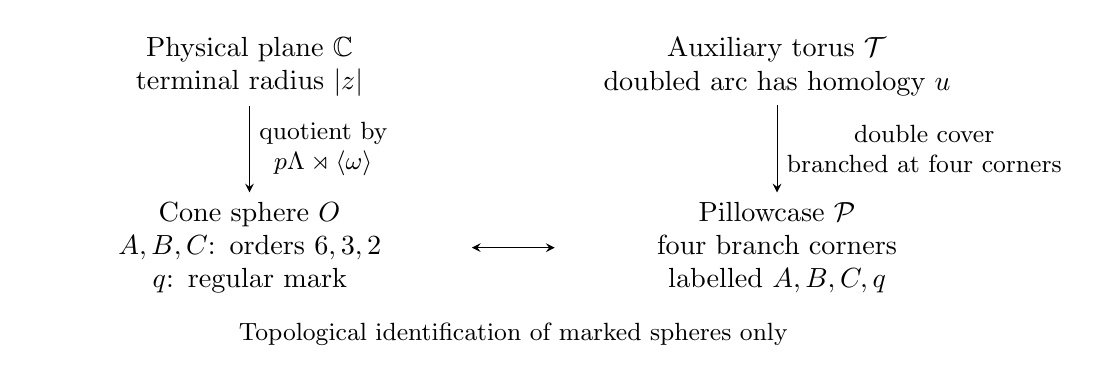
\begin{tikzpicture}[>=stealth, every node/.style={align=center}]
\node[text width=5.4cm] (physical) at (-3.35,2.3)
  {Physical plane \(\mathbb C\)\\terminal radius \(|z|\)};
\node[text width=5.4cm] (cone) at (-3.35,0)
  {Cone sphere \(O\)\\\(A,B,C\): orders \(6,3,2\)\\\(q\): regular mark};
\node[text width=5.4cm] (torus) at (3.35,2.3)
  {Auxiliary torus \(\mathcal T\)\\doubled arc has homology \(u\)};
\node[text width=5.4cm] (pillow) at (3.35,0)
  {Pillowcase \(\mathcal P\)\\four branch corners\\labelled \(A,B,C,q\)};
\draw[->] (physical) -- node[right, font=\small]
  {quotient by\\\(p\Lambda\rtimes\langle\omega\rangle\)} (cone);
\draw[->] (torus) -- node[right, font=\small]
  {double cover\\branched at four corners} (pillow);
\draw[<->] (cone.east) -- (pillow.west);
\node[font=\small] at (0,-1.1)
  {Topological identification of marked spheres only};
\end{tikzpicture}
\caption{The two covering constructions in the radius bound. The auxiliary
torus classifies the endpoint arc by a primitive vector \(u\); its physical
terminal radius is measured in the plane on the left. The identification
of the marked spheres does not identify their metrics or their covers.}
\label{fig:pv:localization-covers}
\end{figure}


Use the tetrahedral triangulation of \(O\) obtained by joining \(q\) to the
three vertices of its flag-triangle face. On \(\mathcal P\), split the two
squares by opposite diagonals, and identify corresponding triangles
affinely. Each bounded physical segment meets boundedly many period tiles
because \(p\ge1\), and boundedly many of their subdivisions. Its image in
each auxiliary triangle is a segment of bounded length. Hence the image of
\(\alpha\) has length polynomial in \(D+1\), uniformly in \(q\). This uses
bounded piece counts and triangle diameters, not a uniform derivative bound
for the affine identifications when a triangle becomes thin.

Lift \(\alpha\) in the auxiliary plane from 0 to an integer point \(u\),
whose parity is the terminal corner. The two lifts in \(\mathcal T\) form a
simple closed curve; a plane lift of this curve runs from 0 to \(2u\).
Its homology vector in the period-2 basis is thus \(u\), and
\(|u|\le (D+2)^{C_0}\) for some absolute \(C_0\). It is nonzero by parity
and primitive: a simple curve of nonzero homology on a torus is
nonseparating, and cutting along it supplies a dual curve of intersection
number one. Notice that \(u\) is not the displacement of the original
physical lift.

The straight segment from 0 to this primitive \(u\) projects to a simple
arc with the same endpoint corners. It has no internal corner, and
\((s\pm t)u\in2\mathbb Z^2\) forces \(s\pm t\in2\mathbb Z\), which rules
out any other identification of its interior points. To compare it with
\(\alpha\), take the boundary of a narrow disk neighborhood of each arc,
containing just its two endpoint marks. Each boundary lifts to a pair of
parallel torus curves of slope \(u\).

Put these two sphere boundaries in minimal transverse position relative to
the four marks. If they intersect, their number of crossings is even and at
least two. Their union has no cut vertex: after deleting any crossing, the
two remaining paths still meet at another crossing. The complementary faces
are therefore disks bounded by simple even-sided polygons, and each bigon
has distinct vertices. Euler's formula gives
\[
 \sum_{\text{faces }F}(4-\#\text{sides of }F)=8.
\]
An unmarked bigon could be removed by an isotopy. Since there are only four
marks, the formula forces exactly four bigons, each containing one mark,
and all other faces to be quadrilaterals. In the branched double cover every
marked bigon becomes a quadrilateral, while each unmarked quadrilateral
lifts to two. The resulting torus has a quadrangulation of valence four.
Gluing unit squares gives a flat torus on which the two curve families run
straight and cross perpendicularly. Its complete simply connected flat
cover develops onto the Euclidean plane; its deck maps are translations,
since they are orientation-preserving and fixed-point-free. The crossing
families consequently have different homological slopes, contradicting
their common slope \(u\).

The boundaries can thus be made disjoint. As they enclose the same pair of
marks, the annulus between them contains no mark, and they are isotopic
relative to the marks. This disk isotopy preserves terminal lift radius in
\(O\). Indeed a disk containing only an endpoint arc and the marks
\(A,q\) lifts above it to disks branched at the preimages of \(A\). In the
component about 0, the only monodromy is rotation about 0; \(q\) is regular.
All arcs in this disk from \(A\) to \(q\) therefore have equal terminal
radius. Such disk neighborhoods apply locally throughout the isotopy, and
the same observation compares the two arcs once they lie in one disk.
Thus the straight auxiliary arc has the same physical terminal radius as
\(\alpha\).

\paragraph{Reducing the shear word by cone monodromy.}
The Euclidean algorithm sends the unit horizontal vector to \(u\) by a
word in powers of the horizontal shear
\(H(x,y)=(x+y,y)\) and quarter turns, with
\(O(1+\log|u|)\) blocks. These integer linear maps act on the pillowcase.
Every shear exponent can be reduced modulo 12 without changing the terminal
physical radius of the final endpoint arc.

To see this, \(H^2\) is isotopic relative to the corners to one Dehn twist
about a curve separating them into pairs. Deform \((x,y)\mapsto(x+2y,y)\)
to \((x,y)\mapsto(x+F(y),y)\), where \(F\) is odd,
\(F(y+2)=F(y)+4\), is flat at \(2k\) near each integer row \(y=k\), and
rises by 2 between successive rows. The two twisting strips on the torus
are identified to one annulus on the pillowcase. For any curve separating
the four marks into pairs, its side containing \(q\) contains exactly one
cone mark. Its monodromy in the physical cover has order dividing 6.
Six twists consequently insert only trivial six-turn based loops at all
crossings of an endpoint arc with the twisting annulus.

When a shear block is replaced inside a word, the final arcs differ by a
conjugate of such a sixfold twist. Its supporting curve still separates the
marks into pairs, and the conjugated twist fixes each mark. This justifies
the reduction for internal blocks as well as terminal ones: the endpoint
marks remain the same at every comparison. The shortened word has length
\(O(\log(D+2))\) in a fixed finite collection of matrix maps.

\paragraph{An additive radius cost for each pure generator.}
Some matrices permute the corners, and these cannot all be lifted as maps
of the physical plane with its differently ordered cones. Separate that
permutation first. Choose fixed representatives for the matrix classes
modulo 2. If \(W=g_1\cdots g_m\) is the shortened word and \(r_i\) represents
the class of \(g_1\cdots g_i\), with \(r_0=1\), then
\[
 h_i=r_{i-1}g_i r_i^{-1},\qquad W=h_1\cdots h_m r_m.
\]
The \(h_i\) belong to a fixed finite collection of pure, corner-fixing
matrices. The representative \(r_m\) acts first on the unit arc; it has the
same corner permutation as \(W\), so the resulting arc runs from \(A\)
to \(q\). Its bounded complexity gives an initial physical radius \(O(p)\).
We do not assert a global physical-plane lift for this nonpure map.

Each pure map, transported to \(O\), does lift to a homeomorphism
\(\widetilde f\) of the physical plane fixing 0. Off the four marks, the
lifting subgroup is normally generated by the peripheral-loop powers of
orders \(6,3,2\), together with the loop about the regular mark \(q\):
upstairs these are circuits of individual punctures. A pure map preserves
these generators up to conjugacy. It therefore preserves the subgroup,
lifts off the punctures, and extends across them by the local cyclic-cover
picture.

Conjugation by \(\widetilde f\) preserves the translation subgroup of the
deck group: its nonidentity elements are exactly the infinite-order deck
transformations. Thus for a real-linear lattice automorphism \(L\),
\begin{equation}\label{eq:pv:pure-lift-equivariance}
 \widetilde f(z+\lambda)=\widetilde f(z)+L\lambda,
 \qquad \lambda\in p\Lambda.
\end{equation}
It also intertwines rotation about 0 by \(\omega\) with rotation by
\(\omega\) or \(\omega^{-1}\). Such a real-linear \(L\) is a similarity;
as it is a lattice automorphism, \(|\det L|=1\), so it is orthogonal.

The remaining bound is on one period cell, uniformly in the regular mark
\(q\). From 0 to a generic point of that cell, choose boundedly many
straight pieces in an \(O(p)\) region, avoiding lifted marks after departure.
They cross boundedly many flag triangles and their subdivisions, even when
some subtriangles are thin. After the affine identification, the path has
boundedly many bounded straight pieces in the auxiliary square model.
Applying a fixed matrix and subdividing again preserves that bound. Mapping
back, every piece lies in a physical triangle of diameter \(O(p)\), so the
path lifts to length \(O(p)\). Limits handle nongeneric points. This also
proves the bounded-complexity estimate for the initial representative arc.
It follows that \(|\widetilde f(z_0)|\le C p\) on a period cell at 0, with
one constant for the finite collection of pure generators.

Write \(z=z_0+\lambda\). Equation
\eqref{eq:pv:pure-lift-equivariance} and orthogonality now give the global
\emph{additive} bound
\[
 |\widetilde f(z)|\le |z|+C'p.
\]
Starting from the representative arc and applying the
\(O(\log(D+2))\) pure lifts, we obtain
\(D-O(1)\le Cp\log(D+2)\). Since \(p\ge1\), this proves the lemma.
\end{proof}

\subsection{Removing oversized polygons}

The geometric lemma also gives a form that will be used for polygons in a
strip. Here a pure lattice period may point in any direction; it need not
be the horizontal period of the original balanced cylinder.

\begin{corollary}\label{cor:pv:oversized-polygons}
Fix \(\delta>0\). Suppose \(\mathcal U\) is a family of planar honeycomb
polygons enclosing 0 whose interiors are disjoint from their nontrivial
translates by a common pure lattice period of length \(p\). For all
sufficiently large \(p\),
\[
 \sum_{\substack{P\in\mathcal U\\
             \max_{z\in P}|z|>p^{1+\delta}}}x_*^{|P|}=O(1).
\]
The constant is independent of the family and the period direction.
\end{corollary}

\begin{proof}
For the geometric argument, rotate coordinates to make the given period
horizontal; the six-rotation lemma is unchanged by this rotation. For the
weighted-degree argument, use an ordinary balanced cylinder in the original
lattice coordinates. Take a finite subset of oversized polygons, of mass
\(B\), and put it and all six lattice rotations into this cylinder with a
sufficiently large circumference, so that every polygon encloses one marked
face and not the other and has its original weight. This containing cylinder
need not have the given period, and its circumference may depend on the
finite subset. Lemma~\ref{lem:pv:weighted-degree} is uniform in that choice.

For two chosen polygons \(P,Q\) with area of \(P\) at least area of \(Q\),
suppose all rotations of \(Q\) are compatible with \(P\). For each rotation,
its Jordan boundary and that of \(P\) are disjoint and enclose 0, so its
closed disk lies strictly inside the disk of \(P\), by the area ordering.
The interior of \(P\) can
therefore serve as \(U\) in Lemma~\ref{lem:pv:six-rotations}, giving
\(D_Q\le Cp\log(D_Q+2)\). For fixed \(\delta>0\) and large \(p\), this
contradicts \(D_Q>p^{1+\delta}\).

The area-ordered pairs have total weight at least \(B^2/2\). Assign to each
one an incompatible rotation of \(Q\). A pair in the union with rotations
has at most six preimages, so its incompatibility numerator is at least
\(B^2/12\), while the union has mass at most \(6B\). The weighted-degree
bound gives \(B\le72r_0^{-1}\). Exhaustion by finite subsets proves the
claim.
\end{proof}

\begin{proof}[Proof of Proposition~\ref{prop:pv:planar-localization}]
On the cylinder of circumference \(p=2n\), essential polygons separating
the marked faces fall into two families, according to which cylinder end
is on the same side as each mark. Opposite families cannot coexist, and
translation by \(n\), swapping the marks, exchanges their weights. If a
finite subset of one family has mass \(B\), its union with its translated
image has mass \(2B\) and incompatibility numerator at least \(2B^2\).
Lemma~\ref{lem:pv:weighted-degree} gives \(B\le r_0^{-1}\). Thus the total
single-polygon weight of essential polygons is \(O(1)\).

Every remaining cylinder polygon is contractible. Lift its disk and
translate the enclosed marked face to 0. Its interior is disjoint from all
nonzero translates by the horizontal period \(p\). For each of the two
marked-face families, Corollary~\ref{cor:pv:oversized-polygons} shows that
the polygons whose lifted radius exceeds \(p^{1+\delta}\) have total weight
\(O(1)\).

For the upper comparison, put two independent planar disk gases of radius
\(cp\), for a fixed sufficiently small \(c>0\), around the two marked
faces. Their disks are disjoint on the cylinder, so all their polygons
qualify and
\begin{equation}\label{eq:pv:disk-cylinder-upper}
 Z(cp)^2\le F_n(2)=n^{1/6+o(1)}.
\end{equation}
For the lower comparison, remove essential and oversized polygons from a
cylinder configuration. Ignoring every avoidance restriction involving the
removed polygons bounds their possible contribution at fugacity 2 by
\[
 \prod_{P\text{ removed}}(1+2w(P))
 \le \exp\left(2\sum_{P\text{ removed}}w(P)\right)=O(1).
\]
The retained polygons lift into the two planar disk systems of radius
\(p^{1+\delta}\). Dropping restrictions between these systems yields
\begin{equation}\label{eq:pv:disk-cylinder-lower}
 F_n(2)\le C_\delta Z(p^{1+\delta})^2.
\end{equation}
The upper comparison gives exponent at most \(1/12\), and the lower one
gives exponent at least \(1/(12(1+\delta))\). Monotonicity fills the radii
between the cylinder scales. First let the radius tend to infinity for
fixed \(\delta\), then let \(\delta\downarrow0\), proving the proposition.
\end{proof}

In the strip application below, a transverse lattice period of length
comparable to the strip height makes each polygon interior period-free.
Corollary~\ref{cor:pv:oversized-polygons} therefore supplies the same
oversized-polygon removal before Proposition~\ref{prop:pv:planar-localization}
is applied to the retained disk system.

\section{Vertex visits and finite chord means}\label{c01-c1-the-two-leg-mass}

The analytic argument has produced a partition function for polygons.
We now insert a visited vertex into a path. The conversion is a finite
exploration identity, valid before any infinite-volume limit. Its
positive expansion will also justify the deletion comparison needed
for the later transfer from arches to bridges.

A finite vertex set $D$ is \emph{filled} if every lattice vertex
strictly inside a simple polygon in its induced honeycomb graph also
belongs to $D$. Boundary ports are midpoints of edges with one endpoint
in $D$ and one outside. An excursion joins two distinct boundary ports
and visits distinct vertices of $D$. We order its endpoints, so
reversal gives a second excursion. For $v\in D$, define
\[
 T_D(v)=\sum_{\gamma\ni v}x_*^{|\gamma|}e^{i\sigma W(\gamma)},
 \qquad \sigma=3/8.
\]
Reversal conjugates each term, so $T_D(v)$ is real. Its individual
terms need not have positive real part in a general filled set.
For a face $f$ incident to $v$, let $Z_D(f)$ be the sum over systems
of vertex-disjoint polygons in $D$ enclosing its center, with weight
$2x_*^{|P|}$ per polygon and with the empty system included.

\begin{proposition}[Finite visit recursion]\label{prop:pv:visits}
For every finite filled vertex set $D$ and $v\in D$,
\begin{align}
 T_D(v)=3
 &+\sum_{\substack{P\subset D\\v\in P}}
 2x_*^{|P|-1}\big[-\cos\big(\sigma(2\pi-\tau_v(P))\big)\big]
 \label{eq:pv:visit-recursion}\\
 &+\sum_{\substack{P\subset D\\v\in P^\circ}}
 2x_*^{|P|}T_{P^\circ}(v).\notag
\end{align}
Here $P^\circ$ is the strict interior vertex set and
$\tau_v(P)\in\{\pi/3,-\pi/3\}$ is the counterclockwise turn at $v$.
Every coefficient on the right is positive. Thus $T_D(v)\ge3$,
it is monotone under inclusion of filled sets containing $v$, and
there are absolute constants $c,C>0$ such that
\[
 c\sum_{f\sim v}Z_D(f)\le T_D(v)\le C\sum_{f\sim v}Z_D(f).
\]
If $D$ is cut out by admissible tiling lines in a convex polygon and
$A_D(v)$ is the positive ordered excursion weight through $v$, then
\[
 \cos(3\pi/8)A_D(v)\le T_D(v)\le A_D(v).
\]
\end{proposition}

\begin{proof}
At a fresh vertex reached along one edge, take either nonbacktracking
continuation with weight $x_*e^{i\sigma\pi/3}$ or
$x_*e^{-i\sigma\pi/3}$. Their sum is one. Stop at an exit port or just
before choosing a continuation at the first repeated vertex. The
exploration tree is finite and replacing a node by its children
preserves total weight. A prefix stopped on first arrival at a vertex
has not yet taken its weight or its turn.

Start at a boundary port. A first repeat consists of a simple stem
followed by a polygon attached at its end. The stem is outside the
polygon: otherwise the outside neighbor of its starting port would
be inside that polygon, contradicting filling. The two orientations
of the polygon add turns $\pm4\pi/3$ relative to the stem. Their
phase sum is $2\cos(4\pi\sigma/3)=0$. This pairing also cancels after
restricting to histories that have visited $v$, because reversal
preserves their vertices. Continuing a first-arrival prefix at $v$
has total terminal weight one. Hence the sum of first-arrival prefixes
equals the excursion weight through $v$. Summing starting ports gives
$T_D(v)$.

Now start at $v$ along each of its three edges, with initial weight one
and with neither weight nor turn at $v$. Stop at an exit, a return to
$v$, or the first repeat of another vertex. The three explorations
have total weight $3$. Their exit terms reverse the prefixes just
counted, so their sum is the conjugate of $T_D(v)$ and hence $T_D(v)$.
A return to $v$ traces a polygon $P$ through it. Its turn omits exactly
$\tau_v(P)$ from the total $2\pi$, and its weight omits exactly one
factor $x_*$. The two orientations therefore contribute
\[
 2x_*^{|P|-1}\cos\big(\sigma(2\pi-\tau_v(P))\big).
\]

For a first repeat away from $v$, let $P$ be the attached polygon. If
$v$ is outside $P$, exterior-stem cancellation applies. If $v$ is
inside, the unused edge at the attachment points into the polygon.
Arriving from the stem replaces the counterclockwise turn $-\pi/3$
there by $+\pi/3$. The two traversals add turns $\pm8\pi/3$,
both with phase $-1$, and contribute $-2x_*^{|P|}$ times the stem
weight. For fixed $P$, these stems are exactly paths from $v$, with
no weight or turn there, to boundary ports of $P^\circ$. Filling gives
$P^\circ\subset D$; planarity shows that an edge leaving its interior
ends on $P$. Completing the last half-edge therefore introduces no
extra weighted vertex. Prefix reversal in this smaller filled set
gives stem sum $T_{P^\circ}(v)$. The terminal balance is
\[
 3=T_D(v)+\sum_{P\ni v}2x_*^{|P|-1}
 \cos\big(\sigma(2\pi-\tau_v(P))\big)
 -\sum_{v\in P^\circ}2x_*^{|P|}T_{P^\circ}(v),
\]
which proves the recursion.

If $P$ encloses one of the three faces incident to $v$, its turn there
is $+\pi/3$; if it encloses two, the turn is $-\pi/3$. The omitted-turn
angles are $5\pi/3$ and $7\pi/3$. Set
\[
 c_1=-\cos(5\pi/8)>0,\qquad c_2=-\cos(7\pi/8)>0.
\]
Iterate the recursion. It terminates since a strict interior has fewer
vertices than its container. The result sums outer-to-inner chains
of disjoint polygons strictly enclosing $v$, with factor $2x_*^{|P|}$
for each. In the final interior $D'$ the remaining multiplier is
\[
 3+\frac2{x_*}\sum_{\substack{Q\subset D'\\v\in Q}}
 c_{m_Q}x_*^{|Q|},\qquad m_Q\in\{1,2\}.
\]
This positive expansion proves both positivity and filled-set
monotonicity: inclusion only adds eligible chains and through-polygons.

The same strict chains enumerate $\sum_{f\sim v}Z_D(f)$. A polygon
strictly enclosing $v$ encloses all three incident face centers. A
polygon through $v$ encloses exactly $m_Q$ of them. Conversely, a
polygon enclosing an incident face has $v$ in its interior or on its
boundary, because the open face does not meet the polygon and
approaches $v$. A vertex-disjoint system has at most one polygon
through $v$, and it must be innermost. Thus its final multiplier is
\[
 3+2\sum_{\substack{Q\subset D'\\v\in Q}}m_Qx_*^{|Q|}.
\]
The two ratios $c_m/(x_*m)$ are fixed positive numbers. Termwise
comparison proves the incident-face bounds.

Finally close a convex-domain excursion by the complementary
counterclockwise boundary arc. Its turn is the lifted change of
outward boundary normal from the initial port to the terminal one,
minus $\pi$. That change lies in $[0,2\pi]$, so $|W|\le\pi$.
Each phased real part is therefore between $\cos(3\pi/8)$ and one
times its positive weight. Summation proves the last assertion.
\end{proof}

The proposition estimates visits without choosing the wall on which
the excursion ends. We first apply it to hexagon chords and mixed
strip exits; only afterward do we isolate bridges.


\subsection{Exponential lateral tails in a strip}

Before normalizing the finite chord laws, we control excursions that
travel sideways while remaining in a thin strip. This estimate also
justifies the subsequent lateral exhaustions with a length insertion.

\begin{lemma}[Lateral tail]\label{lem:pv:lateral-tail}
Consider critical exits from a fixed bottom port in a strip of $h$
layers, or in a convex tiling-line truncation of that strip. Let
$X(\gamma)$ be the largest horizontal distance of a visited vertex
from the source. There are absolute constants $C,c>0$ such that
\[
 \sum_{X(\gamma)\ge t}x_*^{|\gamma|}
 \le C\exp\{-ct/(h+1)\}\qquad(t\ge0).
\]
The same bound, with a polynomial prefactor, holds with a first-length
insertion. In particular the contribution with
$X\ge h\log^2h$ to any first-length mass is smaller than every
fixed inverse power of $h$ as $h\to\infty$.
\end{lemma}

\begin{proof}
For the right tail, take two further tiling cuts with outward normals
$(\sqrt3/2,1/2)$ and $(\sqrt3/2,-1/2)$, in coordinates along and
above the bottom side. Let $E_+,E_-$ be the sets of old exits lost when
the corresponding half-plane is imposed. Flux subtraction puts their
phased sums on the distinct rays
$e^{-i\sigma\pi/3}$ and $e^{-2i\sigma\pi/3}$: the turn from the
source to a new cut is fixed. Differently directed cuts do not share
ports. Since vertical coordinates range over $O(h+1)$, their
intercepts can be staggered by $O(h+1)$ and rounded to the tiling grid
so that
\[
 \{X_+>r+C(h+1)\}\subset E_-\subset E_+
 \subset\{X_+>r\},
\]
where $X_+$ is maximum rightward displacement. All old exit weights
have phased real parts comparable to their positive weights by
convexity. Separation of the two rays implies that the absolute
weight of $E_+\setminus E_-$ is at least a fixed positive fraction
of the weight of $E_-$. This gives fixed-factor decay in each
increment $C(h+1)$, starting from the uniformly bounded total exit
mass. Reflection gives the left tail.

In this subtraction, an exit is lost exactly when it visits a removed
vertex. A newly clipped exit attempts such a vertex along the new
cut; an old exit still valid contributes identically to the two flux
sums, even if its port belongs to both boundaries. Thus no boundary
term was omitted by the nesting of the cuts. The constants are
uniform in a convex lateral truncation, and monotone exhaustion
gives the full-strip statement.

Finally a simple path in $h$ layers and horizontal range $X$ visits
at most $C(h+1)(X+1)$ vertices. The tail integral of the preceding
exponential bound consequently gives, after adjusting $C,c$,
\[
 \sum_{X(\gamma)\ge t}|\gamma|x_*^{|\gamma|}
 \le C(h+1)(h+t+1)e^{-ct/(h+1)}.
\]
At $t=h\log^2h$ this is smaller than any fixed power of $h^{-1}$.
\end{proof}


\subsection{Macroscopic chords in a hexagon}\label{sec:pv:hexagon-proof}

For specificity take regular lattice hexagons of integer side \(R\to\infty\). Say an arc is macroscopic when its diameter is at least \(R/10\). Their absolute critical mass over all boundary sources is
\[
 R^{3/4+o(1)}.
\]
For the lower bound use sources in the central third of one side. Exits not to the initial bottom side all have macroscopic reach. Flux and comparison of bottom returns with arches in a containing flat strip of \(O(R)\) layers give non-bottom mass at least \(b_{O(R)}\).

For the upper bound per source, impose a cut parallel to its starting side at height $h=\lfloor R/\log^2R\rfloor$. Flux subtraction bounds the mass of exits removed by this cut by a constant times $b_h$, since its new exit prefixes are strip bridges. A retained macroscopic path must reach horizontal distance comparable to $R$, so Lemma~\ref{lem:pv:lateral-tail} bounds its weight by $Ce^{-c\log^2R}$. Summing over the $O(R)$ boundary sources proves the upper normalizing exponent.

Under the normalized macroscopic arc weights, bulk vertices (say in the central third) now have visit probability
\[
 R^{-2/3+o(1)}.
\]
Indeed all visiting paths there qualify, and the surrounding-polygon sums in Proposition~\ref{prop:pv:visits} lie between disk sums at comparable radii. Proposition~\ref{prop:pv:planar-localization} gives their exponent. The same upper bound holds throughout the hexagon. Summing the probabilities yields the mean visited mass, or length,
\[
 \mathbb E |\gamma|=R^{4/3+o(1)} .
\]

\subsection{A fixed-source strip version}\label{c01-c1-a-fixed-source-strip-version}

There is also an annealed dimension statement with one actual boundary point fixed. In the full planar strip of \(h\) layers take all the critical exits from a fixed bottom port (thus bridges to the top \textbf{or} arches back to bottom), conditioned to get at least one quarter of the way up. Then
\[
 \mathbb E |\gamma|=h^{4/3+o(1)} .
\]
Changing this to any fixed positive fraction strictly below one half gives the same result. The exit mass of this ensemble before normalization is \(h^{-1/4+o(1)}\): lower by the bridges, upper for the arches by the height-tail bound. This conditioning could also confine horizontal range to \(h\log^2 h\) about the start without changing the exponent. For bridges alone the argument gives the mean upper bound \(h^{4/3+o(1)}\) (and hence the usual in-probability upper-exponent bound), not by itself the matching bridge lower bound.

The pointwise estimate behind this statement will also be needed for the
bridge lower bound. It sums over all boundary positions, rather than
fixing a source.

\begin{lemma}[Strip visit weights]\label{lem:pv:strip-visits}
Let $A_{S_h}(v)$ be the positive weight of ordered strip excursions
through $v$, with both endpoints free on the two horizontal boundaries.
Uniformly over strip vertices,
\[
 A_{S_h}(v)\le h^{1/12+o(1)}.
\]
For every fixed $\delta>0$, uniformly over vertices at least
$\delta h$ layers from both horizontal boundaries,
\[
 A_{S_h}(v)=h^{1/12+o(1)}.
\]
The same upper bound holds for the ordered excursion weight $A_D(v)$
in every convex lateral truncation $D$, including excursions with
lateral endpoints. Its lower bound holds uniformly when, in addition
to the horizontal clearance above, $v$ is at distance at least
$\delta h$ from every lateral side.
\end{lemma}

\begin{proof}
Convexly truncate the strip at lateral distance $W$ on both sides using
tiling lines of the two slanted side orientations. For a face within
bounded distance of the strip, fugacity-$2$ systems using strip vertices
and surrounding that face have sum at most $h^{1/12+o(1)}$, uniformly in
the truncation. Indeed every enclosing polygon interior lies in the
slab and is disjoint from its translates by nonzero multiples of
$p\omega$, for a sufficiently large integral $p\asymp h$.
Corollary~\ref{cor:pv:oversized-polygons} applies to this transverse
period: its geometric argument rotates the period direction to
horizontal, while its degree bound uses a sufficiently large balanced
cylinder containing any finite test subset and all its rotations. Loops of
radius greater than $p^{1+\alpha}$ therefore cost at most a bounded
exponential factor. The remaining loops are controlled by
Proposition~\ref{prop:pv:planar-localization}. First let $h\to\infty$
for fixed $\alpha>0$, then let
$\alpha\downarrow0$. For faces at least a fixed multiple of $h$ from
the walls and the lateral ends, an inscribed disk gives the matching lower
exponent.

Proposition~\ref{prop:pv:visits} now gives both estimates in every
finite convex truncation. We also need a tail bound for its side
sources. Use the two slanted tiling cuts facing toward the far part of
the strip, with both outward normals pointing laterally that way.
Their distinct angles from the initial inward direction lie strictly
between $-\pi$ and $\pi$, so the separated-ray argument of
Lemma~\ref{lem:pv:lateral-tail} bounds the weight reaching lateral
distance $t$ by $Ce^{-ct/(h+1)}$. Displacement toward the near end is
limited by $O(h+1)$, and length is bounded by
$C(h+1)(1+\text{lateral span})$. Thus each side source has bounded
length mass at fixed $h$, uniformly in the truncation width.

Let $W\to\infty$ at fixed $h$. Excursions between horizontal boundary
ports exhaust the strip excursions. For a fixed marked vertex, paths
from the $O(h)$ distant side ports have vanishing weight by the same
tail bound. This proves the stated full-strip estimates.
\end{proof}

We finish Proposition~\ref{prop:pv:mixed} by averaging over horizontal
sources. In a finite truncation $D$, counting every visited vertex gives
the exact identity
\[
 \sum_{v\in D} A_D(v)
 =\sum_{\gamma\text{ an ordered excursion in }D}
   |\gamma|x_*^{|\gamma|}.
\]
Divide by horizontal width and let that width tend to infinity at fixed
$h$. Lemma~\ref{lem:pv:strip-visits} bounds the result above by
$h^{13/12+o(1)}$. A central band of $\asymp h$ layers supplies the same
lower exponent. For the ensemble conditioned to reach $\vartheta h$
layers above its starting wall, where $0<\vartheta<1/2$ is fixed,
choose this band symmetric about the midline and more than
$\vartheta h$ layers from either wall. Every
path contributing a visit to that band then meets the conditioning
event, from either horizontal starting side.

The slanted side sources disappear in this average: there are only
$O(h)$ of them, and the tail estimate in the preceding proof bounds
each one's length mass at fixed $h$. Their contribution divided by
width therefore vanishes.

Each horizontal wall has one source port per unit length. Translation
invariance and top--bottom symmetry therefore identify the limiting
average with twice the fixed-source length weight. One can first
restrict to bounded path range, pass to
the large-width limit, and then remove that restriction using the
exponential tails. Thus the conditioned ensemble has unnormalized
length weight $h^{13/12+o(1)}$. Its mass is $h^{-1/4+o(1)}$ by
Proposition~\ref{prop:pv:boundary}, giving the asserted mean. The same
tails make the discarded first moment at horizontal range
$h\log^2 h$ smaller than every fixed power of $h$, proving the optional
confinement statement.

\section{A marked tripod comparison for bridge mass}\label{c01-c1-transfer-to-bridges}

We have proved the mixed exit mean, but its length mass might still be carried mainly by arches returning to the same wall. This section proves that crossing bridges retain the bulk visit exponent and completes Theorem~\ref{thm:pv:bridge}. The first step is an exact comparison of intersecting pairs, obtained by marking a tripod. The second is a geometric lower bound on how many translates of bridges hit a deep arch. Fix a vertex \(v\) in the central third of the strip of \(h\) layers. Sum over all boundary positions here. Count each bridge once (say bottom to top); let \(m\) be their weight through \(v\). Count each same-side arch on either boundary also once, with total weight through \(v\) denoted by \(u\). Absolute weights are always products of \(x_*\) per visited vertex. Write
\[
 \theta=\pi/8,\quad k=\cos\theta,\quad c=\cos(3\theta)=\sin\theta,\quad
 p=e^{i\theta},\quad g=\cos(2\theta),\quad \phi=2g-1=c/k .
\]
\subsection{Deletion and first contact}

An active outer path is phased by \(\exp(i\sigma W)\) as before. It may be stopped just before first attempting entry to \(v\), without using a weight there; call such prefixes \(\eta\). The phased full exits through \(v\) sum to the sum on these prefixes by deletion flux. Likewise for first hit (meaning first attempted vertex, not taking its weight) of another obstacle. For disjoint obstacles \(v,X\), the phased sum of full exits hitting both equals the sum of prefixes to first \(X\) that have visited \(v\), plus prefixes to first \(v\) that have visited \(X\): just use deletion for \(v,X,v\cup X\). All actual path intersections below mean shared visited vertices.

At fixed \(h\) these operations in the unbounded strip can be done by absolute convergence. Indeed embed the strip by projection into a tilted cylinder, with a period along another tiling direction and large enough vertical shift for injectivity on the strip. On that cylinder strip-bridge weights in the longitudinal direction decay exponentially in the number of layers, as above. All SAWs from a fixed vertex there have absolutely summable critical weights with exponential tails in longitudinal span \(D\): lengths are \(O_h(D+1)\), and the weak-bridge unfolding count (decomposition at extremal heights on the two halves, as above) uses subexponentially many lists with sublinear number of spans, whose sum is at least \(D\). Positive weak bridges again extend by boundedly many vertices to cut lines without repetitions and each costs at most a constant times exponential decay in its span. Thus the loss besides that exponential is subexponential. This gives absolute convergence also with polynomial factors and for connected finite products of paths with one site anchored. Flux calculations can equivalently truncate laterally first (also when a fixed finite crosscut is removed).

Let \(J\) be the absolute sum for a bridge and an arch (arch counted once, on either side) intersecting each other with at least one through \(v\), and \(J_{CC}\) the analogous ordered sum for two bridges. Each pair receives the product of its two path weights, so a vertex shared by the two independently chosen paths occurs in both factors. These sums are finite by the anchored convergence just proved. Our first target is
\begin{equation}\label{eq:pv:pair-target}
 J\le C(J_{CC}+m).
\end{equation}
Once this comparison is established, lateral tails will bound $J_{CC}$ in terms of $m$, while translations will bound $J$ below in terms of $u$. The following complex sums are introduced solely to prove \eqref{eq:pv:pair-target}.

\subsection{The marked tripod identity}

Use triples of boundary ports \(a,b,c'\), where \(b<c'\) are ordered on one horizontal side and \(a\) is on the opposite. Positive order is east along the bottom, reversed along the top. We sum over both choices of side. A tripod consists of simple arms from these ports to a center vertex, mutually disjoint until the center, all weights included there once, the arm turn \(W_j\) from \(j\) measured up to arrival (before turning at the center). By planarity their cyclic order is forced. Since joining \(b\) to \(a\) or \(c'\) to \(a\) forms a bridge (turn zero in total), and the join turns are \(+\pi/3,-\pi/3\) respectively,
\[
 e^{i\sigma W_a}=p\,e^{i\sigma W_b}=\bar p\,e^{i\sigma W_{c'}}.
\]
Figure~\ref{fig:pv:tripod} shows the first-contact construction. Only the cyclic order, rather than the pictured shape, enters the phase relations.
\begin{figure}[tb]
\centering
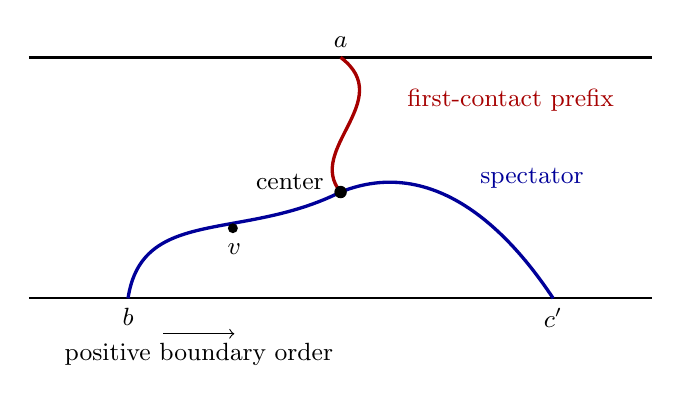
\begin{tikzpicture}[scale=.9, every node/.style={font=\small}]
 \draw[thick] (-.4,0)--(8.4,0);
 \draw[thick] (-.4,3.4)--(8.4,3.4);
 \node[below] at (1,0) {$b$};
 \node[below] at (7,0) {$c'$};
 \node[above] at (4,3.4) {$a$};
 \draw[very thick,blue!60!black] (1,0)
  .. controls (1.2,1.3) and (2.6,.8) .. (4,1.5);
 \draw[very thick,blue!60!black] (4,1.5)
  .. controls (5.5,2.1) and (6.6,.6) .. (7,0);
 \draw[very thick,red!65!black] (4,3.4)
  .. controls (4.8,2.8) and (3.5,2.1) .. (4,1.5);
 \fill (4,1.5) circle (2.5pt);
 \node[left] at (3.9,1.65) {center};
 \fill (2.48,.99) circle (2pt);
 \node[below] at (2.5,.91) {$v$};
 \node[blue!60!black] at (6.7,1.7) {spectator};
 \node[red!65!black] at (6.4,2.8) {first-contact prefix};
 \draw[->] (1.5,-.5)--(2.5,-.5);
 \node[below] at (2,-.5) {positive boundary order};
\end{tikzpicture}
\caption{A contact tripod, shown schematically. The arch from $b$ to
$c'$ is the spectator and a prefix from the opposite port $a$ reaches
it for the first time at the center. The center is weighted once.
Reassigning the active arm gives the two bridge-spectator terms.
The vertex $v$ may lie on any arm or at the center; the restrictions
in the proof keep these cases separate.}
\label{fig:pv:tripod}
\end{figure}


Let \(L_*\) sum all tripods containing \(v\), using the first (common) phase \(e^{i\sigma W_a}\).

The following sums use independent spectator and active paths, with
only the active path phased. A full exit includes all its visited
vertex weights; a prefix $\eta$ stops just before $v$ and omits its
weight. The port order and the sum over both choices of side are as
above.
\begin{center}
\small
\renewcommand{\arraystretch}{1.15}
\begin{tabular}{@{}p{.09\textwidth}p{.35\textwidth}p{.48\textwidth}@{}}
\toprule
Sum & Spectator & Active path and contact condition\\
\midrule
$A$ & Arch $b\to c'$ containing $v$
 & Full exit from $a$, hitting the spectator\\
$E_A$ & Arch $b\to c'$ avoiding $v$
 & Full exit from $a$, hitting both the spectator and $v$\\
$R_A$ & Arch $b\to c'$ avoiding $v$
 & Prefix $\eta$ from $a$, hitting the spectator before its stop\\
\midrule
$Z_b$ & Bridge $c'\to a$ containing $v$
 & Full exit from $b$, hitting the spectator\\
$Z_{c'}$ & Bridge $b\to a$ containing $v$
 & Full exit from $c'$, hitting the spectator\\
\midrule
$E_C$ & Bridge avoiding $v$, counted once
 & Full exit from any boundary source, hitting the spectator and $v$\\
$R_C$ & Bridge avoiding $v$, counted once
 & Prefix $\eta$ from any boundary source, hitting the spectator\\
\bottomrule
\end{tabular}
\end{center}
Set $Z=Z_b+Z_{c'}$. In $E_C$ and $R_C$, the active source may lie
on either boundary and may coincide with a spectator endpoint.

Hitting a marked spectator is represented by first contact by deletion. This gives exactly the contact tripod weights; in particular \(A,p Z_b,\bar p Z_{c'}\) in common phase restrict \(L_*\) to \(v\) not exclusively on the open arm \(a,b,c'\), respectively. The contact representation uses the free third edge for the incoming active prefix, since its source differs from the spectator endpoints. When the spectator avoids \(v\), the term in which \(v\) is visited before first contact is instead the complementary restriction in \(L_*\), with phase depending on the active arm. Thus
\[
 R_A=E_A+A-L_*,\qquad R_C=E_C+Z-2k L_*.
\]
This uses the both-obstacles formula above; if the active source coincides with a bridge spectator endpoint, all exits and prefixes to \(v\) hit that spectator with no possible \(v\) before first contact, consistent with the second equation.

For another balance, let the spectator now be a prefix $\eta$ from the
top weighted with \emph{conjugate} phase, and grow the opposite active
path in $S\setminus\{v\}$. Its valid ends are an original outer
boundary port or an attempt at $v$, stopped before taking its weight.
Revisit pairs from an outer source still cancel, with or without
deleting the spectator vertices. Use also the bottom spectator and top
active balance, add, and take real parts. The real sum of products for
valid leaves hitting those spectators is
\[
 \Re(2c R_A+R_C)+2P,\qquad
 P=\Re\!\!\sum_{\eta_B\cap\eta_T\ne\varnothing}
 w(\eta_B) w(\eta_T) e^{i\sigma(W_B-W_T)}
\]
where subscripts denote the lower/upper source and $w$ denotes absolute
path weight. Outer leaves are arches avoiding $v$ (both orientations,
averaging to phase $c$) or bridges avoiding $v$ (phase $1$); the other
leaves are the intersecting prefixes.

Write $u_B,u_T$ for the once-counted arch weights through $v$ on the
bottom and top, so $u=u_B+u_T$. By deletion, the two full prefix sums
are the nonnegative real numbers
\[
 M_B=m+2cu_B,\qquad M_T=m+2cu_T.
\]
Disjoint opposite-side prefixes join at $v$ to give each bridge through
$v$ once. Their product omits exactly the weight $x_*$ at $v$, and
their arrival-turn difference is $\pm\pi/3$, with real phase $k$.
Subtracting these disjoint pairs from the full product gives
\begin{equation}\label{eq:pv:prefix-product}
 P=M_BM_T-\frac{k}{x_*}m\ge-\frac{k}{x_*}m.
\end{equation}

At first contact the two shoulders from opposite sides form a bridge
$\lambda$ avoiding $v$. The incoming active edge is free: neither the
edge toward the spectator's source nor the edge toward its stopped-at
$v$ could have brought the opposite active path to its first contact.
The spectator suffix starts along the third edge from the center and
goes to $v$, avoiding $\lambda$. The bridge takes the center weight
once; the suffix takes neither that weight nor the weight at $v$.
Conversely these objects give all contacts once per choice of active
side.

Write $\delta=\pm\pi/3$ for the bottom-to-top join turn at the center,
and $W'$ for the suffix turn starting along its outgoing edge. The
shoulder-turn difference is $-\delta$; the turn into the suffix from
the top is $\delta$, and from the bottom $-\delta$. The two phase
factors therefore add to $2g e^{-i\sigma W'}$. For fixed $\lambda$,
the real suffix sum without $2g$ is exactly the real sum of prefixes
to $v$ in $S-\lambda$ from the new boundary ports on the unused
outward edges of $\lambda$. Length zero is included when appropriate.

Write $H(S;v)$ and $H(S-\lambda;v)$ for the real prefix sums to $v$
from the respective whole boundaries. Original prefixes avoiding
$\lambda$ are unchanged, so the new-boundary suffix sum equals the
original-boundary prefix sum hitting $\lambda$, minus
\[
 \Delta_\lambda=H(S;v)-H(S-\lambda;v)\ge0.
\]
For the inequality, reverse to exits from $v$ and use the positive
nesting expansion of Proposition~\ref{prop:pv:visits}, whose final
multipliers are $3+(2/x_*)\sum_Q c_{m_Q}w(Q)$. The domain $S-\lambda$
is filled: a removed bridge connected to the outer boundary cannot
enter the strict interior of a polygon avoiding it. For fixed
$\lambda$, take the nesting comparison first in convex lateral
truncations with and without its vertices, and then pass to the strip;
side contributions anchored at $v$ vanish by the convergence already
proved. When summing $w(\lambda)\Delta_\lambda$, use its representation
as hit prefixes minus new-boundary prefixes. Both are connected
terms; no sum of disconnected boundary terms is needed.
The first-contact calculation consequently gives
\[
 \Re(2cR_A+R_C)+2P=2g\left[\Re R_C-\sum_{\lambda\not\ni v}w(\lambda)\Delta_\lambda\right].
\]
Using the earlier equations (the \(L_*\) terms cancel since \(\phi k=c\)),
\[
 2c\Re(A+E_A)+2P\le \phi\Re(E_C+Z).
\]

\subsection{Comparison of intersecting path pairs}

We now compare the phased expressions with the positive pair sums.
Including only bridge exits as active paths gives $\Re(A+E_A)\ge J$;
the remaining exits have positive real weights. Also
$\Re(E_C+Z)\le2cJ+2J_{CC}$: allow active sources coinciding with a
marked spectator endpoint, adding nonnegative real weight, and combine
both orientations of every active path. Together with
\eqref{eq:pv:prefix-product}, the last phased inequality becomes
\[
 2c(1-\phi)J\le2\phi J_{CC}+\frac{2k}{x_*}m.
\]
Since $\phi<1$, this proves \eqref{eq:pv:pair-target}.

Let $\mu_h$ be the unnormalized measure on bottom-to-top bridge shapes
from one fixed bottom port, of total mass $b_h$. Write $X(\beta)$ for
the largest horizontal distance of a visited vertex from that source,
as in Lemma~\ref{lem:pv:lateral-tail}, and set $T=h\log^2h$ for large
$h$. If both bridge shapes have $X\le T$, then for any fixed marked
bridge the other shape has at most $CT$ translations hitting it.
Choosing which member contains $v$ only changes the constant. Thus
\[
 J_{CC}\le CTb_hm+R_h,
\]
where $R_h$ is the contribution of pairs with at least one $X>T$.

We bound this remainder absolutely, without an estimate on $m$.
A fixed-source shape $\beta_1$ has at most $|\beta_1|$ translations
placing a visited vertex at $v$, and
$|\beta_1|\le C(h+1)(X_1+1)$, where $X_i=X(\beta_i)$.
For each such translate, a second shape has at most
$C(X_1+X_2+1)$ translations hitting it. Hence, uniformly in $v$,
\begin{align*}
 R_h&\le C(h+1)
 \iint_{\max(X_1,X_2)>T}(1+X_1+X_2)^2
 \,d\mu_h(\beta_1)\,d\mu_h(\beta_2)\\
 &\le C(h+1)(T+h+1)^2e^{-cT/(h+1)}=O(h^{-100}).
\end{align*}
The second line follows by integrating the exponential tail in
Lemma~\ref{lem:pv:lateral-tail} for the first two moments of $X$,
using $b_h\le1$ and splitting according to which $X_i>T$.
Since $b_h=h^{-1/4+o(1)}$, we obtain
\begin{equation}\label{eq:pv:bridge-pair-upper}
 J_{CC}\le h^{3/4+o(1)}m+O(h^{-100}).
\end{equation}

\subsection{Translation hits on a deep arch}

The upper pair bound pays one bridge crossing mass for each allowed
horizontal translation. We need a matching lower bound for bridges
hitting each arch through the marked vertex. Here the error must be
uniform in the arch, whose length and horizontal span are unrestricted.

\begin{lemma}[Translated bridge hits]\label{lem:pv:translation-hits}
Let $\alpha$ be any same-side arch meeting the central third of the
strip. Let $\mathcal H_h(\alpha)$ be the total weight of strip bridges,
summed over all bottom sources, that intersect $\alpha$. For every
fixed $\epsilon\in(0,1)$,
\[
 \mathcal H_h(\alpha)\ge h^{3/4-\epsilon-o(1)},
\]
uniformly over all such arches. In particular
$\mathcal H_h(\alpha)\ge h^{3/4-o(1)}$ uniformly.
\end{lemma}

\begin{proof}
By reflection in the strip midline, it suffices to treat a bottom
arch. Translate its start to the fixed bottom source, put
$W=h^{1-\epsilon}$, and consider its prefix up to first crossing
layer $r=\lfloor h/4\rfloor$. Such a crossing exists because the arch
meets the central third.

\emph{Equal-height contact intervals.}
We first compare two prefixes $\alpha_0,\beta_0$ from the bottom to
their first crossings of the same cut. Parametrize them on $[0,1]$;
their heights lie strictly between the two cut heights internally.
There is a compact connected set of equal-height parameter pairs
containing $(0,0)$ and $(1,1)$, whose projections onto both parameter
intervals are all of $[0,1]$. Consequently its horizontal-difference
image is an interval of translations giving contact. It contains the
start and final offsets, and also an offset matching any prescribed
point on either prefix with a point on the other.

This is the piecewise-linear mountain-climbing construction
\cite[Theorem~5.5]{Pak2010}; we give the contact argument needed here.
On the parameter square, triangulate so that the height difference is
piecewise linear. For sufficiently small positive regular values its
level set has exactly two boundary endpoints, near the diagonal
corners, joined by an arc. Indeed the two prefix heights are strictly
monotone near their extremal endpoints and stay away from these
extremal heights on every compact interior parameter interval.
A subsequential Hausdorff limit of the compact arcs is connected,
lies in the zero set, and contains both corners. Such a subsequence
can also be obtained by diagonal selection of the dyadic boxes met by
the arcs. Each coordinate projection is connected and contains $0$
and $1$, hence equals $[0,1]$. Taking horizontal differences proves
the interval assertion. At integer translations, geometric contact
of the lattice walks gives a shared vertex. A contact at the
intermediate cut is also a shared vertex of the full walks, since
that port lies inside their lattice edges.

\emph{Two direct alternatives.}
Suppose first that at some intermediate cut the arch prefix has two
crossings at horizontal distance at least $W$. Every bridge shape
then has at least $W-O(1)$ hitting translates. To see this, use the
bridge crosscut's left/right side indicator at the two points, with
any fixed convention for points on it. Their separation is an integer.
Summing the signed indicator difference over integer translates
telescopes to that integer in absolute value. Any discrepancy forces
the intervening arch segment to meet the bridge. Summing bridge
shapes therefore gives hitting mass at least $(W-O(1))b_h$.

Suppose next that the arch's displacement $a$ at first crossing of
some layer $1,\ldots,r$ satisfies $|a|\ge W$. A bridge and its
reflection about its start have first-crossing displacements $d$ and
$-d$ there, and
\[
 \max\{|a-d|,|a+d|\}\ge |a|\ge W.
\]
For at least one member of this reflection pair, the contact interval
between the start and final offsets yields $W-O(1)$ hitting
translates. Reflection preserves weights, so again the hitting mass
is at least a constant times $Wb_h$.

In the remaining case every first-crossing displacement is less than
$W$ and every same-cut crossing spread is less than $W$. Thus all
cut crossings of the arch prefix lie within $2W$ of its start.
The full prefix stays within $2W+O(1)$: inside a cut-to-cut layer a
walk between ports follows the internal zigzag monotonically.

\emph{Wide bridge prefixes against a confined arch.}
We will show that fixed-source bridges of weight at least
$h^{-1/4-o(1)}$ make lateral distance greater than $4W$ before their
first crossing of layer $r$. We first bound the exceptional confined
pieces that enter the marking argument.

For $h/10\le j\le h/6$, let $e_j$ be the weight of fixed-source
$j$-bridges confined to lateral distance $4W$ from their start. Then
\begin{equation}\label{eq:pv:tube-exception}
 e_j\le C\exp(-ch/W).
\end{equation}
Surround the width-$8W$ tube by a tube of width $O(W)$ whose side
walls alternate the two slanted upward tiling steps between successive
horizontal layers, outside the desired confinement with a safety
margin. Join these walls horizontally on top and bottom. Starting
east along the positive bottom boundary, its unwrapped tangent
angles stay in $[0,2\pi]$: on the right wall they are
$\pi/3,2\pi/3$, and on the left $4\pi/3,5\pi/3$. For a bottom
source, closing an exit by the boundary gives turn $B-\pi$, where
$B\in[0,2\pi]$ is the cumulative tangent turn from source to exit.
Thus all original exits have turns in $[-\pi,\pi]$ and positive
comparable real weights. This supplies the needed positivity even
though the tube is not convex.

Now cut by lines with the two slanted upward normals, of angles
$\pm\pi/3$ from vertical. Boundary-source leaf cancellation still
holds after either cut, since a polygon cannot surround the bottom
source. The genuinely new exits lie on the cut and stay in the convex
wedge between its half-plane and the half-plane above the bottom,
so their turns are fixed. The lost exit sums consequently lie on two
separated rays. Place the intercepts at the source's lateral
coordinate near $s+C'(W+1)$, stagger them by $O(W+1)$, and round to
tiling lines. Since all lateral coordinates are restricted to
$O(W+1)$, the two lost events are nested between reaching heights
$s+C(W+1)$ and $s$. The separated-ray argument of
Lemma~\ref{lem:pv:lateral-tail}, with the positive original exit
weights just established, gives fixed-factor decay per such height
increment, starting at $O(W+1)$. The confined $j$-bridges are among
the top exits of this tube. This proves
\eqref{eq:pv:tube-exception}.

Under the fixed-source bridge measure $\mu_h$ defined above, let
$N(\gamma)$ count layers
$j\in[\lceil h/10\rceil,\lfloor h/6\rfloor]$ that it crosses
exactly once and whose initial $j$-bridge reaches lateral distance
greater than $4W$. At a single-crossing cut, the two bridge pieces
occupy disjoint open slabs. Their weights multiply exactly, since
ports carry no weight. Proposition~\ref{prop:pv:boundary} and
\eqref{eq:pv:tube-exception} give
\begin{align*}
 \int N\,d\mu_h
 &=\sum_j b_{h-j}(b_j-e_j)=h^{1/2+o(1)},\\
 \int N^2\,d\mu_h
 &\le2\sum_{j_1\le j_2}
 b_{j_1}b_{j_2-j_1}b_{h-j_2}
 \le h^{5/4+o(1)}.
\end{align*}
For the second line, dropping the lateral excursion restrictions
leaves three bridge pieces. Use $b_0=1$ on the diagonal and
$\sum_{d\le h}b_d=h^{3/4+o(1)}$; the two outside factors each have
order $h^{-1/4+o(1)}$, uniformly over the chosen layers. Hence
unnormalized Cauchy--Schwarz yields
\[
 \mu_h(N>0)\ge
 \frac{\big(\int N\,d\mu_h\big)^2}{\int N^2\,d\mu_h}
 \ge h^{-1/4-o(1)}.
\]
Every bridge counted here has the required lateral excursion before
first crossing $r$. Apply the contact-interval construction to the
two prefixes ending at $r$, matching that prescribed excursion point
of the bridge to the confined arch prefix. The resulting offset
differs from the initial offset by at least $2W-O(1)$, and hence gives
at least order $W$ integer hitting translates. Their total weight is
at least $W h^{-1/4-o(1)}=h^{3/4-\epsilon-o(1)}$.

All three alternatives give this bound with constants and errors
independent of the arch. For each fixed $\epsilon$, first let
$h\to\infty$; only then let $\epsilon\downarrow0$. This proves the
uniform exponent assertion.
\end{proof}

\subsection{The bridge first moment}

Lemma~\ref{lem:pv:translation-hits} gives
$J\ge h^{3/4-o(1)}u$. Combining this with
\eqref{eq:pv:pair-target} and \eqref{eq:pv:bridge-pair-upper} yields
\[
 u\le h^{o(1)}m+O\big(h^{-100-3/4+o(1)}\big).
\]
On the other hand, $2(u+m)=A_{S_h}(v)$: the ordered excursion
convention counts each path twice. Lemma~\ref{lem:pv:strip-visits}
therefore gives $u+m=h^{1/12+o(1)}$ in the central third, uniformly
in $v$. The negligible additive error above cannot carry this mass,
so
\begin{align*}
 m(v)&=h^{1/12+o(1)}
 &&\text{uniformly in the central third},\\
 m(v)&\le h^{1/12+o(1)}
 &&\text{throughout the strip}.
\end{align*}

To pass from a marked vertex to a fixed source, let $\mathcal V_h$
contain one representative of each horizontal-translation orbit of
strip vertices. Translating a bridge's bottom source to the fixed
source identifies $m(v)$ with the weighted number of visits to the
orbit of $v$. Thus the unnormalized fixed-source length mass is
exactly
\[
 \ell_h=\sum_{v\in\mathcal V_h}m(v).
\]
There are $O(h)$ such orbits, with order $h$ represented in the
central third. The pointwise upper and lower estimates give
$\ell_h=h^{13/12+o(1)}$. Finally, dividing by
$b_h=h^{-1/4+o(1)}$ gives
\[
 \mathbb E|\gamma|=\frac{\ell_h}{b_h}=h^{4/3+o(1)}.
\]
Lemma~\ref{lem:pv:lateral-tail} makes both the discarded mass and
discarded first moment at horizontal range $h\log^2h$ negligible,
so the same conclusion holds with that confinement. This completes
Theorem~\ref{thm:pv:bridge}.

\begin{thebibliography}{99}
\setlength{\itemsep}{2pt plus 1pt minus 0.5pt}
\setlength{\parsep}{0pt}
\setlength{\parskip}{0pt}
\bibitem{BatchelorYung1995}
M.~T.~Batchelor and C.~M.~Yung.
Exact results for the adsorption of a flexible self-avoiding polymer chain
in two dimensions.
\emph{Physical Review Letters} \textbf{74} (1995), 2026--2029.
\href{https://doi.org/10.1103/PhysRevLett.74.2026}{doi:10.1103/PhysRevLett.74.2026}.
\href{https://arxiv.org/abs/cond-mat/9410082v2}{arXiv:cond-mat/9410082v2}.

\bibitem{BeatonEtAl2014}
N.~R.~Beaton, M.~Bousquet-M\'elou, J.~de Gier, H.~Duminil-Copin and A.~J.~Guttmann.
The critical fugacity for surface adsorption of self-avoiding walks on the
honeycomb lattice is $1+\sqrt2$.
\emph{Communications in Mathematical Physics} \textbf{326} (2014), 727--754.
\href{https://doi.org/10.1007/s00220-014-1896-1}{doi:10.1007/s00220-014-1896-1}.
\href{https://arxiv.org/abs/1109.0358v5}{arXiv:1109.0358v5}.

\bibitem{BleherFokin2006}
P.~M.~Bleher and V.~V.~Fokin.
Exact solution of the six-vertex model with domain wall boundary conditions.
Disordered phase.
\emph{Communications in Mathematical Physics} \textbf{268} (2006), 223--284.
\href{https://doi.org/10.1007/s00220-006-0097-y}{doi:10.1007/s00220-006-0097-y}.
\href{https://arxiv.org/abs/math-ph/0510033v3}{arXiv:math-ph/0510033v3}.

\bibitem{BorodinOkounkov2000}
A.~Borodin and A.~Okounkov.
A Fredholm determinant formula for Toeplitz determinants.
\emph{Integral Equations and Operator Theory} \textbf{37} (2000), 386--396.
\href{https://doi.org/10.1007/BF01192827}{doi:10.1007/BF01192827}.
\href{https://arxiv.org/abs/math/9907165}{arXiv:math/9907165}.

\bibitem{DiFrancescoZinnJustin2005}
P.~Di Francesco and P.~Zinn-Justin.
Around the Razumov--Stroganov conjecture: proof of a multi-parameter sum rule.
\emph{Electronic Journal of Combinatorics} \textbf{12} (2005), Research Paper~6.
\href{https://doi.org/10.37236/1903}{doi:10.37236/1903}.
\href{https://arxiv.org/abs/math-ph/0410061}{arXiv:math-ph/0410061}.

\bibitem{DuminilCopinSmirnov2012}
H.~Duminil-Copin and S.~Smirnov.
The connective constant of the honeycomb lattice equals $\sqrt{2+\sqrt2}$.
\emph{Annals of Mathematics} \textbf{175} (2012), 1653--1665.
\href{https://doi.org/10.4007/annals.2012.175.3.14}{doi:10.4007/annals.2012.175.3.14}.

\bibitem{FarbMargalit2012}
B.~Farb and D.~Margalit.
\emph{A Primer on Mapping Class Groups}.
Princeton Mathematical Series, vol.~49.
Princeton University Press, 2012.

\bibitem{FernandezProcacci2007}
R.~Fern\'andez and A.~Procacci.
Cluster expansion for abstract polymer models. New bounds from an old approach.
\emph{Communications in Mathematical Physics} \textbf{274} (2007), 123--140.
\href{https://doi.org/10.1007/s00220-007-0279-2}{doi:10.1007/s00220-007-0279-2}.

\bibitem{Frenkel1981}
I.~B. Frenkel,
\emph{Two constructions of affine Lie algebra representations and
boson--fermion correspondence in quantum field theory},
J. Funct. Anal. \textbf{44} (1981), no.~3, 259--327.
\href{https://doi.org/10.1016/0022-1236(81)90012-4}{doi:10.1016/0022-1236(81)90012-4}.

\bibitem{FrenkelJingWang2000}
I.~B. Frenkel, N. Jing and W. Wang,
\emph{Vertex representations via finite groups and the McKay correspondence},
Internat. Math. Res. Notices \textbf{2000} (2000), no.~4, 195--222.
\href{https://doi.org/10.1155/S107379280000012X}{doi:10.1155/S107379280000012X}.
\href{https://arxiv.org/abs/math/9907166v2}{arXiv:math/9907166v2}.

\bibitem{GarbaliNienhuis2017Ground}
A.~Garbali and B.~Nienhuis.
The dilute Temperley--Lieb $O(n=1)$ loop model on a semi infinite strip:
the ground state.
\emph{Journal of Statistical Mechanics: Theory and Experiment} (2017), 043108.
\href{https://doi.org/10.1088/1742-5468/aa6a30}{doi:10.1088/1742-5468/aa6a30}.
\href{https://arxiv.org/abs/1411.7020}{arXiv:1411.7020}.

\bibitem{GarbaliNienhuis2017Sum}
A.~Garbali and B.~Nienhuis.
The dilute Temperley--Lieb $O(n=1)$ loop model on a semi infinite strip:
the sum rule.
\emph{Journal of Statistical Mechanics: Theory and Experiment} (2017), 053102.
\href{https://doi.org/10.1088/1742-5468/aa6bc3}{doi:10.1088/1742-5468/aa6bc3}.
\href{https://arxiv.org/abs/1411.7160}{arXiv:1411.7160}.

\bibitem{GlazmanManolescu2017}
A.~Glazman and I.~Manolescu.
Self-avoiding walk on $\mathbb Z^2$ with Yang--Baxter weights:
universality of critical fugacity and 2-point function.
\emph{Annales de l'Institut Henri Poincar\'e, Probabilit\'es et Statistiques}
\textbf{56} (2020), 2281--2300.
\href{https://doi.org/10.1214/19-AIHP1024}{doi:10.1214/19-AIHP1024}.

\bibitem{GreeneZaslavsky1983}
C.~Greene and T.~Zaslavsky.
On the interpretation of Whitney numbers through arrangements of hyperplanes,
zonotopes, non-Radon partitions, and orientations of graphs.
\emph{Transactions of the American Mathematical Society} \textbf{280} (1983), 97--126.
\href{https://doi.org/10.1090/S0002-9947-1983-0712251-1}{doi:10.1090/S0002-9947-1983-0712251-1}.

\bibitem{GrimmPearce1993}
U.~Grimm and P.~A.~Pearce.
Multi-colour braid--monoid algebras.
\emph{Journal of Physics A: Mathematical and General} \textbf{26} (1993), 7435--7460.
\href{https://doi.org/10.1088/0305-4470/26/24/018}{doi:10.1088/0305-4470/26/24/018}.
\href{https://arxiv.org/abs/hep-th/9303161}{arXiv:hep-th/9303161}.

\bibitem{HammersleyWelsh1962}
J.~M.~Hammersley and D.~J.~A.~Welsh.
Further results on the rate of convergence to the connective constant of
the hypercubical lattice.
\emph{Quarterly Journal of Mathematics} \textbf{13} (1962), 108--110.
\href{https://doi.org/10.1093/qmath/13.1.108}{doi:10.1093/qmath/13.1.108}.

\bibitem{KrachunPanagiotis2026}
D.~Krachun and C.~Panagiotis.
Quantitative sub-ballisticity of self-avoiding walk on the hexagonal lattice.
\emph{Annals of Probability} \textbf{54} (2026), no.~3, 1109--1125.
\href{https://doi.org/10.1214/24-AOP1730}{doi:10.1214/24-AOP1730}.
\href{https://arxiv.org/abs/2310.17299v1}{arXiv:2310.17299v1}.

\bibitem{MorinDuchesnePearce2019}
A.~Morin-Duchesne and P.~A.~Pearce.
Fusion hierarchies, $T$-systems and $Y$-systems for the dilute $A_2^{(2)}$
loop models.
\emph{Journal of Statistical Mechanics: Theory and Experiment} (2019), 094007.
\href{https://doi.org/10.1088/1742-5468/ab3412}{doi:10.1088/1742-5468/ab3412}.
\href{https://arxiv.org/abs/1905.07973v1}{arXiv:1905.07973v1}.

\bibitem{Nienhuis1982}
B.~Nienhuis.
Exact critical point and critical exponents of $O(n)$ models in two dimensions.
\emph{Physical Review Letters} \textbf{49} (1982), 1062--1065.
\href{https://doi.org/10.1103/PhysRevLett.49.1062}{doi:10.1103/PhysRevLett.49.1062}.

\bibitem{DiskTransfer2026}
OpenAI.
Disk transfer representations and confined bridge mass.
OpenAI Math Release preprint
\href{https://github.com/openai/math/blob/main/preprints/Disk-transfer-representations-and-confined-bridge-mass-September-26-2026/main.pdf}{OAI:Disk-transfer-representations-and-confined-bridge-mass-September-26-2026},
2026.

\bibitem{Pak2010}
I.~Pak.
\emph{Lectures on Discrete and Polyhedral Geometry}.
Lecture notes, April 20, 2010.
\url{https://www.math.ucla.edu/~pak/geompol8.pdf}.

\bibitem{TracyWidom1998}
C.~A.~Tracy and H.~Widom.
Correlation functions, cluster functions and spacing distributions for random matrices.
\emph{Journal of Statistical Physics} \textbf{92} (1998), 809--835.
\href{https://doi.org/10.1023/A:1023084324803}{doi:10.1023/A:1023084324803}.

\bibitem{WarnaarPearceSeatonNienhuis1994}
S.~O.~Warnaar, P.~A.~Pearce, K.~A.~Seaton and B.~Nienhuis.
Order parameters of the dilute $A$ models.
\emph{Journal of Statistical Physics} \textbf{74} (1994), 469--531.
\href{https://doi.org/10.1007/BF02188569}{doi:10.1007/BF02188569}.
\href{https://arxiv.org/abs/hep-th/9305134}{arXiv:hep-th/9305134}.

\bibitem{ZhouBatchelor1997}
Y.~K.~Zhou and M.~T.~Batchelor.
Critical behaviour of the dilute $O(n)$, Izergin--Korepin and dilute
$A_L$ face models: Bulk properties.
\emph{Nuclear Physics B} \textbf{485} (1997), 646--664.
\href{https://doi.org/10.1016/S0550-3213(96)00654-2}{doi:10.1016/S0550-3213(96)00654-2}.
\href{https://arxiv.org/abs/cond-mat/9611156}{arXiv:cond-mat/9611156}.

\end{thebibliography}
\end{document}
